
\clearpage

\section {Results of the $\bar{\nu}/\nu$ joint analysis with the Run 1-6 dataset}
\label{sec:results}

The results of the Run 1-6 data set fit
for an exposure 
of \TotalPotNu POT in neutrino mode
and
of \TotalPotNuBar POT in antineutrino mode 
is shown in this chapter.
In \cref{fig:spectra_expVsdata_asimov_A} the predicted spectra of $\mu$-like and $e$-like samples
are compared to the observed data.
In \cref{tab:num_events} the expected and observed number of events in Run 1-6 data set are shown.
The predicted number of events are shown for the oscillation parameters in \cref{tab:osc_params_joint_asimov}
of Asimov data sets A and B.
All the predicted and observed events are in good agreement.
A small excess of events with respect to the expectation is observed in 
the neutrino mode $e$-like samples, though it is still within $1\sigma$ of the statistical uncertainty.
This trend is mostly inherited from the Run 1-4 data set, since only 2 neutrino mode $e$-like events
are observed in Run 5+6.
Furthermore the latest global fit of the reactor experiments 
gives a lower value of $\sin^2 \theta_{13}$ 
with a much smaller uncertainty (see Sec.~\ref{sec:systematics:inputs} and Tab.~\ref{tab:osc_params_joint_asimov}).
It is interesting to see that the number of events of antineutrino mode $e$-like events 
is in perfect agreement with the assumption of $\delta_{CP} = -1.601$,
which is the best-fit value of the Run 1-4 data set. 
This means that, for what concerns the event rate, we expect to see
agreement between neutrino and antineutrino mode data in the fit of $\delta_{CP}$,
though the statistics are not expected to be enough to reject 
$\delta_{CP}=0$ at any significant confidence level.  

The comparison of the confidence intervals obtained by the fit of the Run 1-6 data set
among all the oscillation analysis groups is shown in \cite{Mach3JointFitRun16}.


\clearpage

% Expected distributions with data overlapped

\begin{figure}
\center
%
\includegraphics[width=0.9\textwidth]{./images/missing_plot-eps-converted-to.pdf}
%
\includegraphics[width=0.9\textwidth]{./images/missing_plot-eps-converted-to.pdf}
%
\includegraphics[width=0.9\textwidth]{./images/missing_plot-eps-converted-to.pdf}
%
\includegraphics[width=0.9\textwidth]{./images/missing_plot-eps-converted-to.pdf}
\begin{subfigure}[b]{0.49\textwidth}
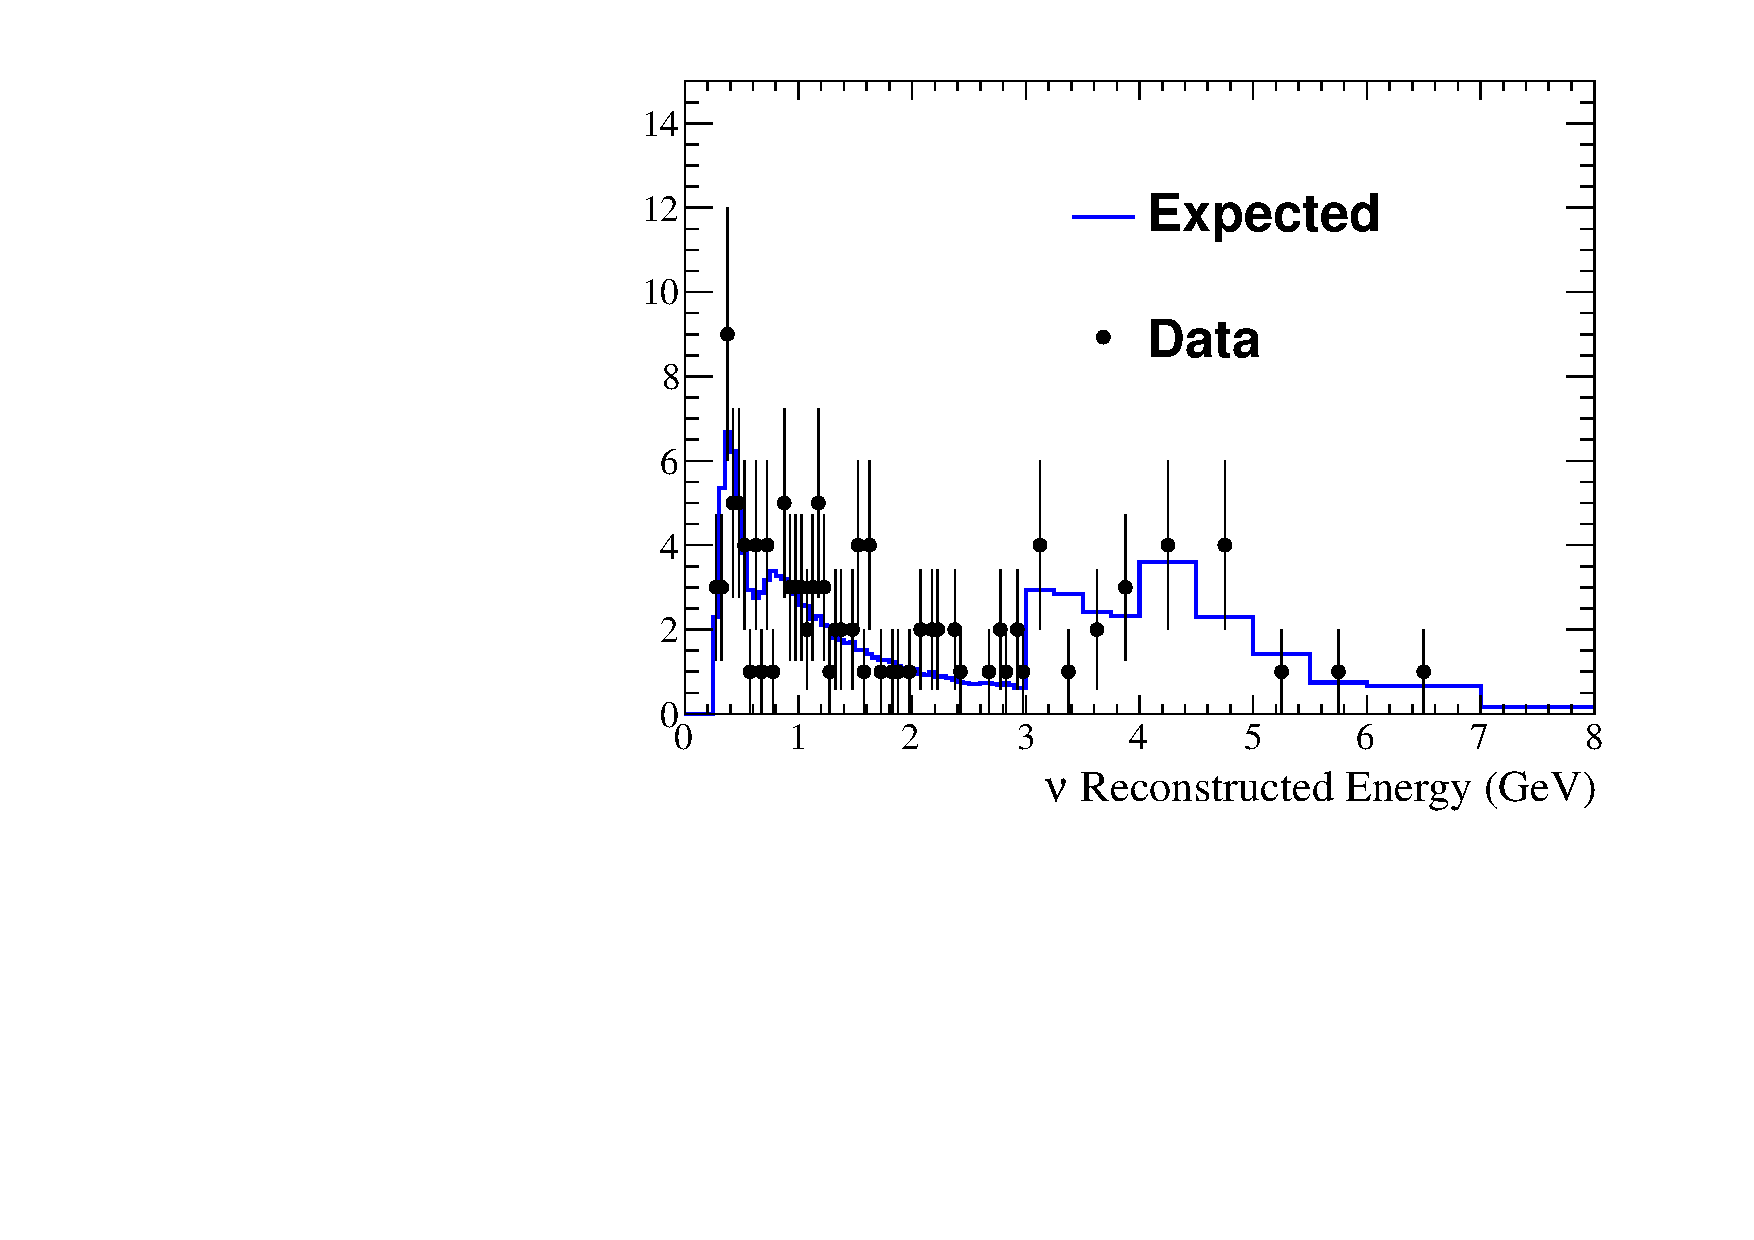
\includegraphics[width=0.9\textwidth]{./joint_plots/data/data_mc_1rmu_tot.pdf}
\caption{Muon-like, neutrino mode}
\end{subfigure}
\begin{subfigure}[b]{0.49\textwidth}
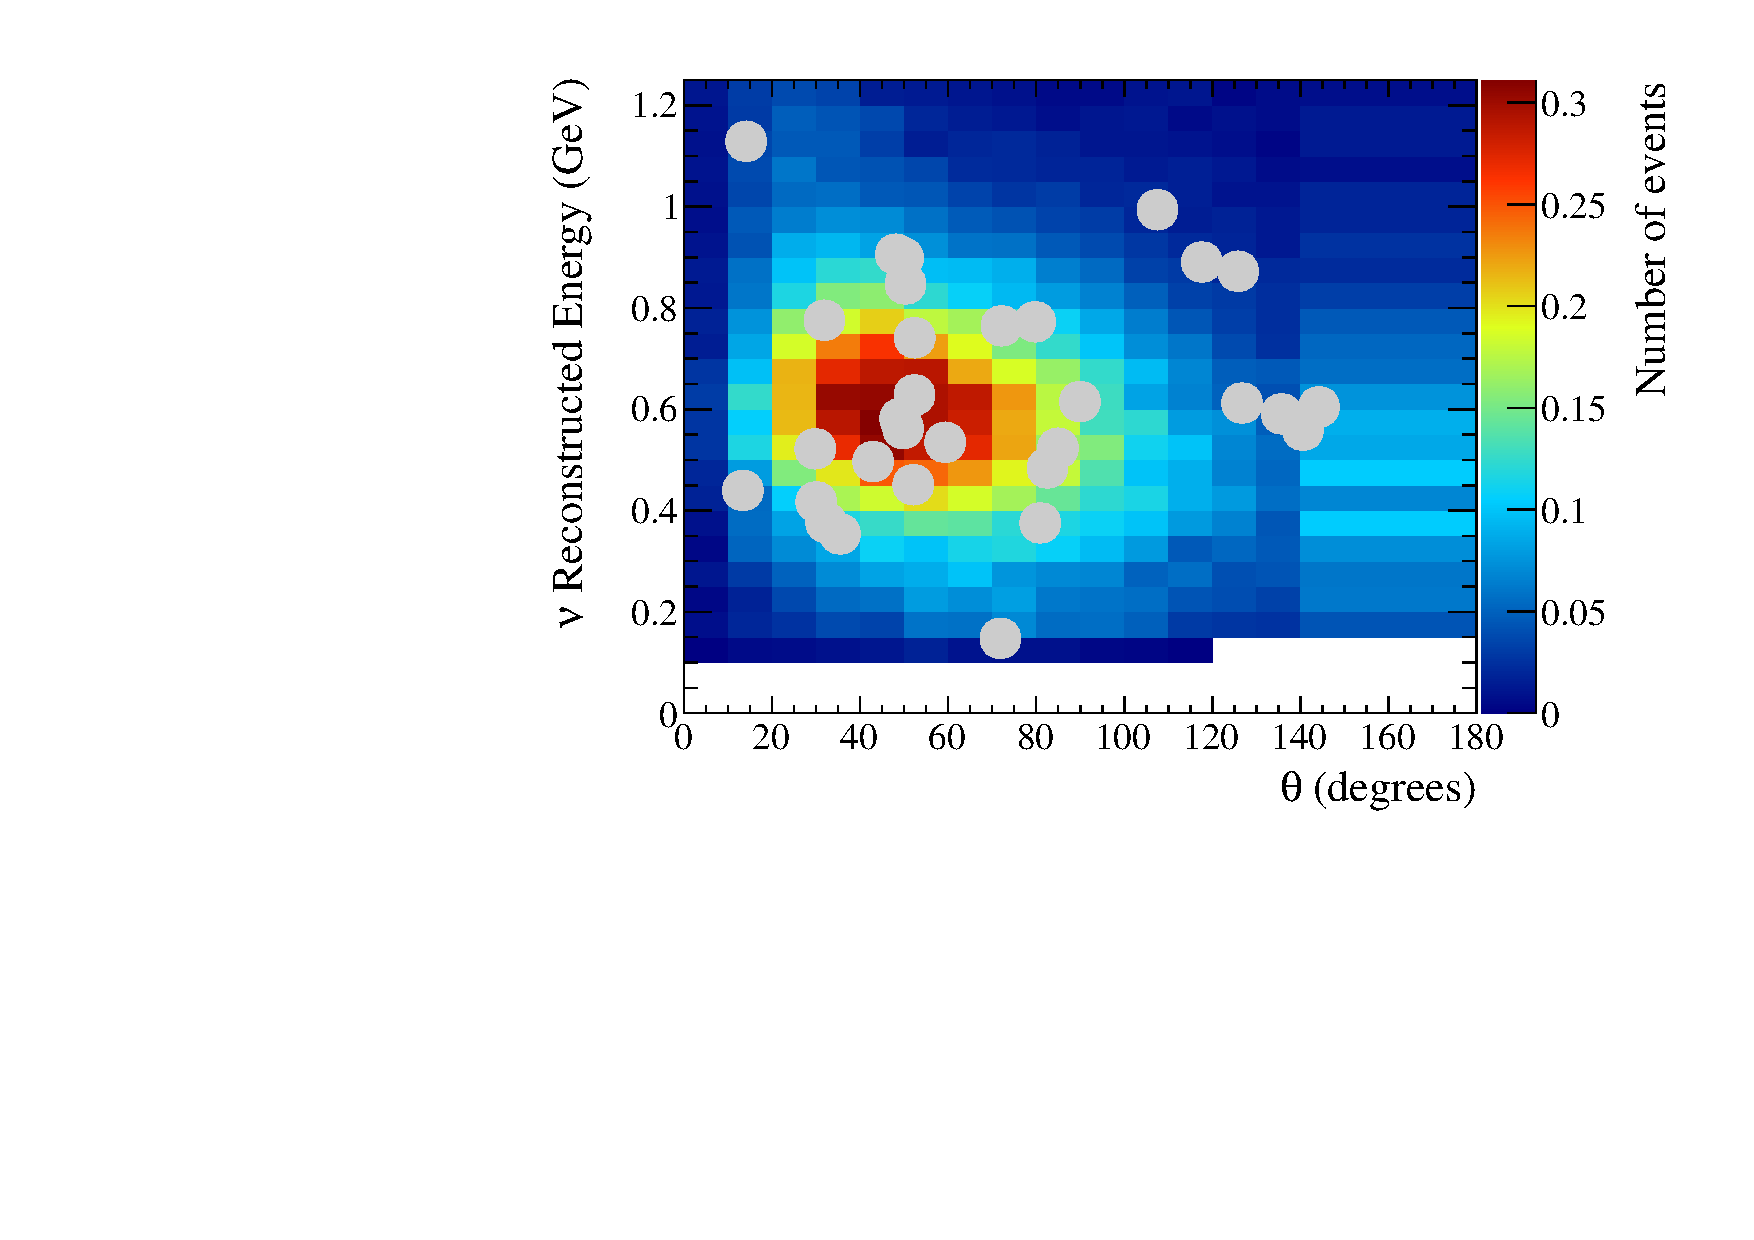
\includegraphics[width=0.9\textwidth]{./joint_plots/data/data_mc_1re_2d_tot.pdf} 
\caption{Electron-like, neutrino mode}
\end{subfigure}
\begin{subfigure}[b]{0.49\textwidth}
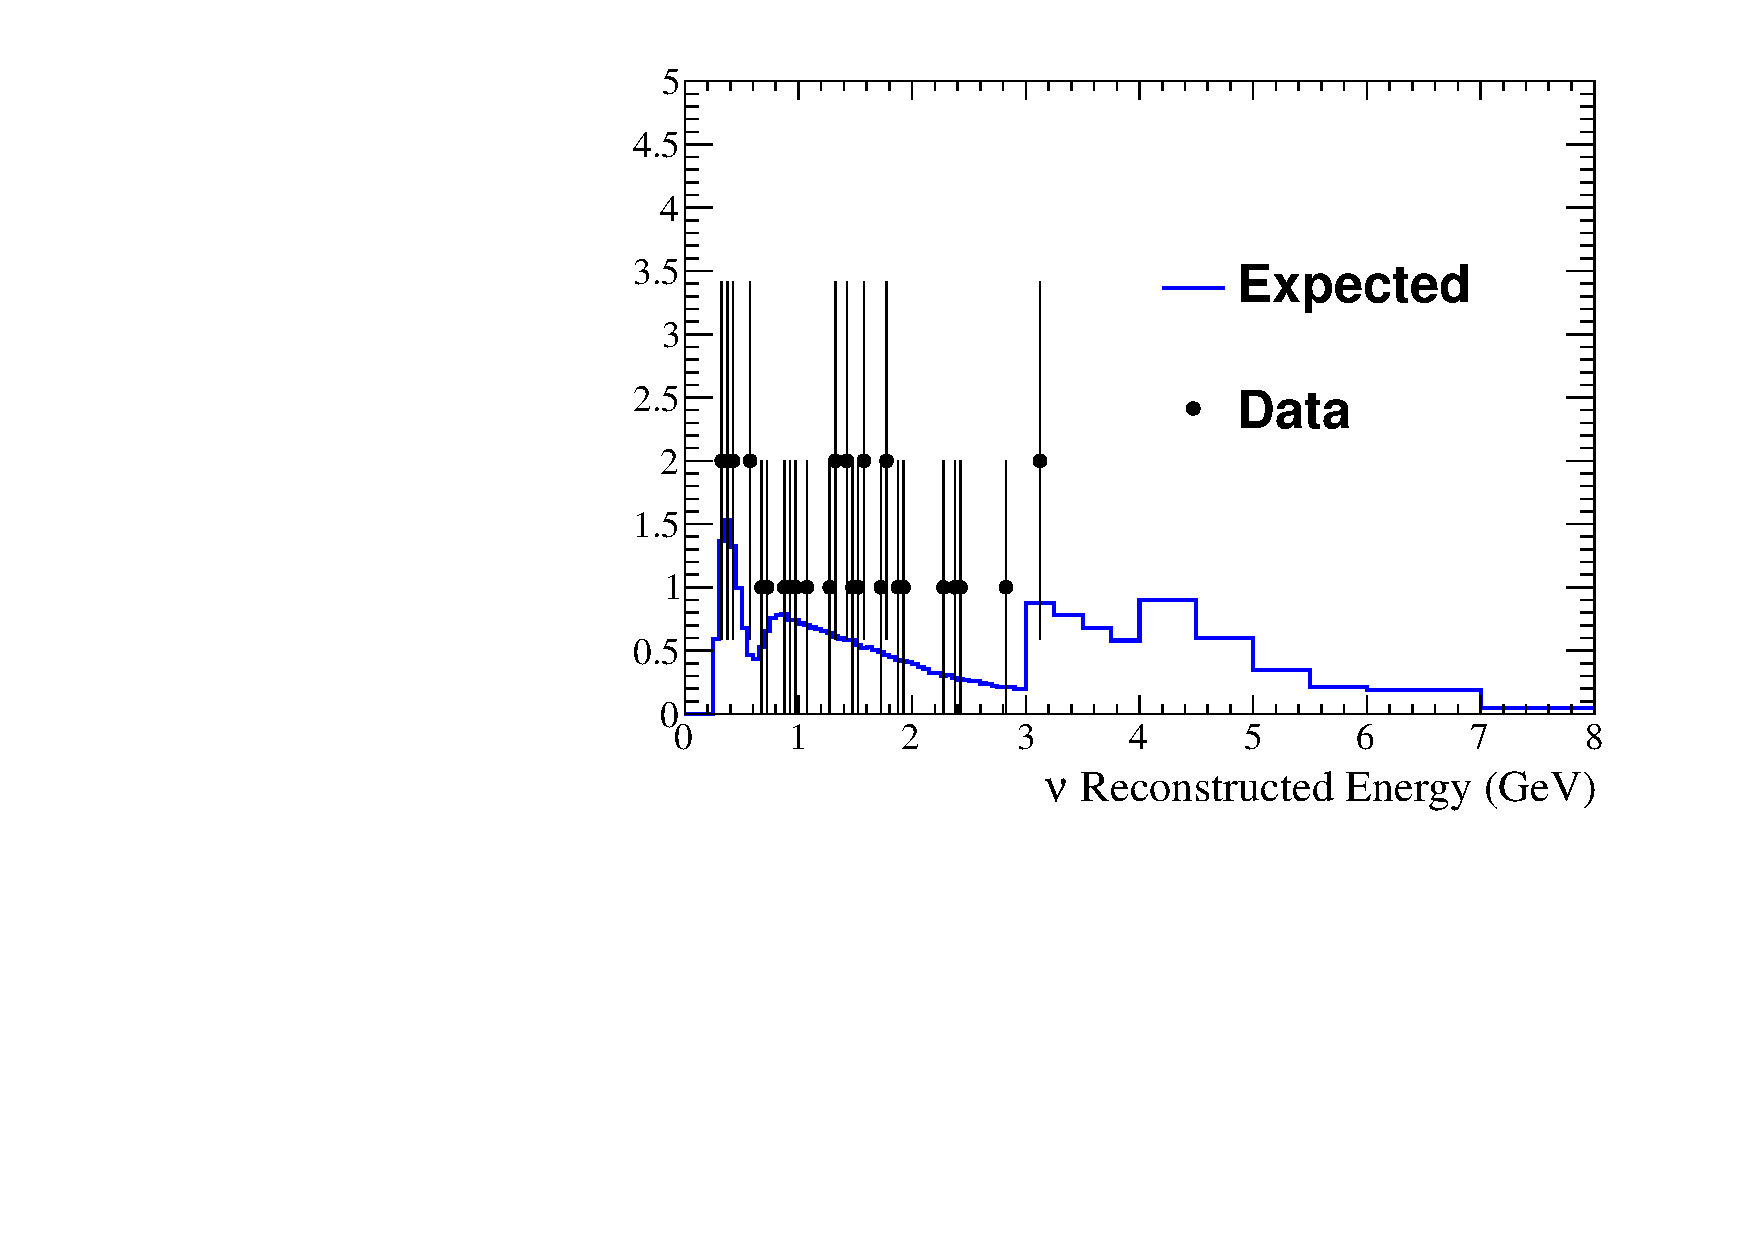
\includegraphics[width=0.9\textwidth]{./joint_plots/data/data_mc_rhc1rmu_tot.pdf}
\caption{Muon-like, antineutrino mode}
\end{subfigure}
\begin{subfigure}[b]{0.49\textwidth}
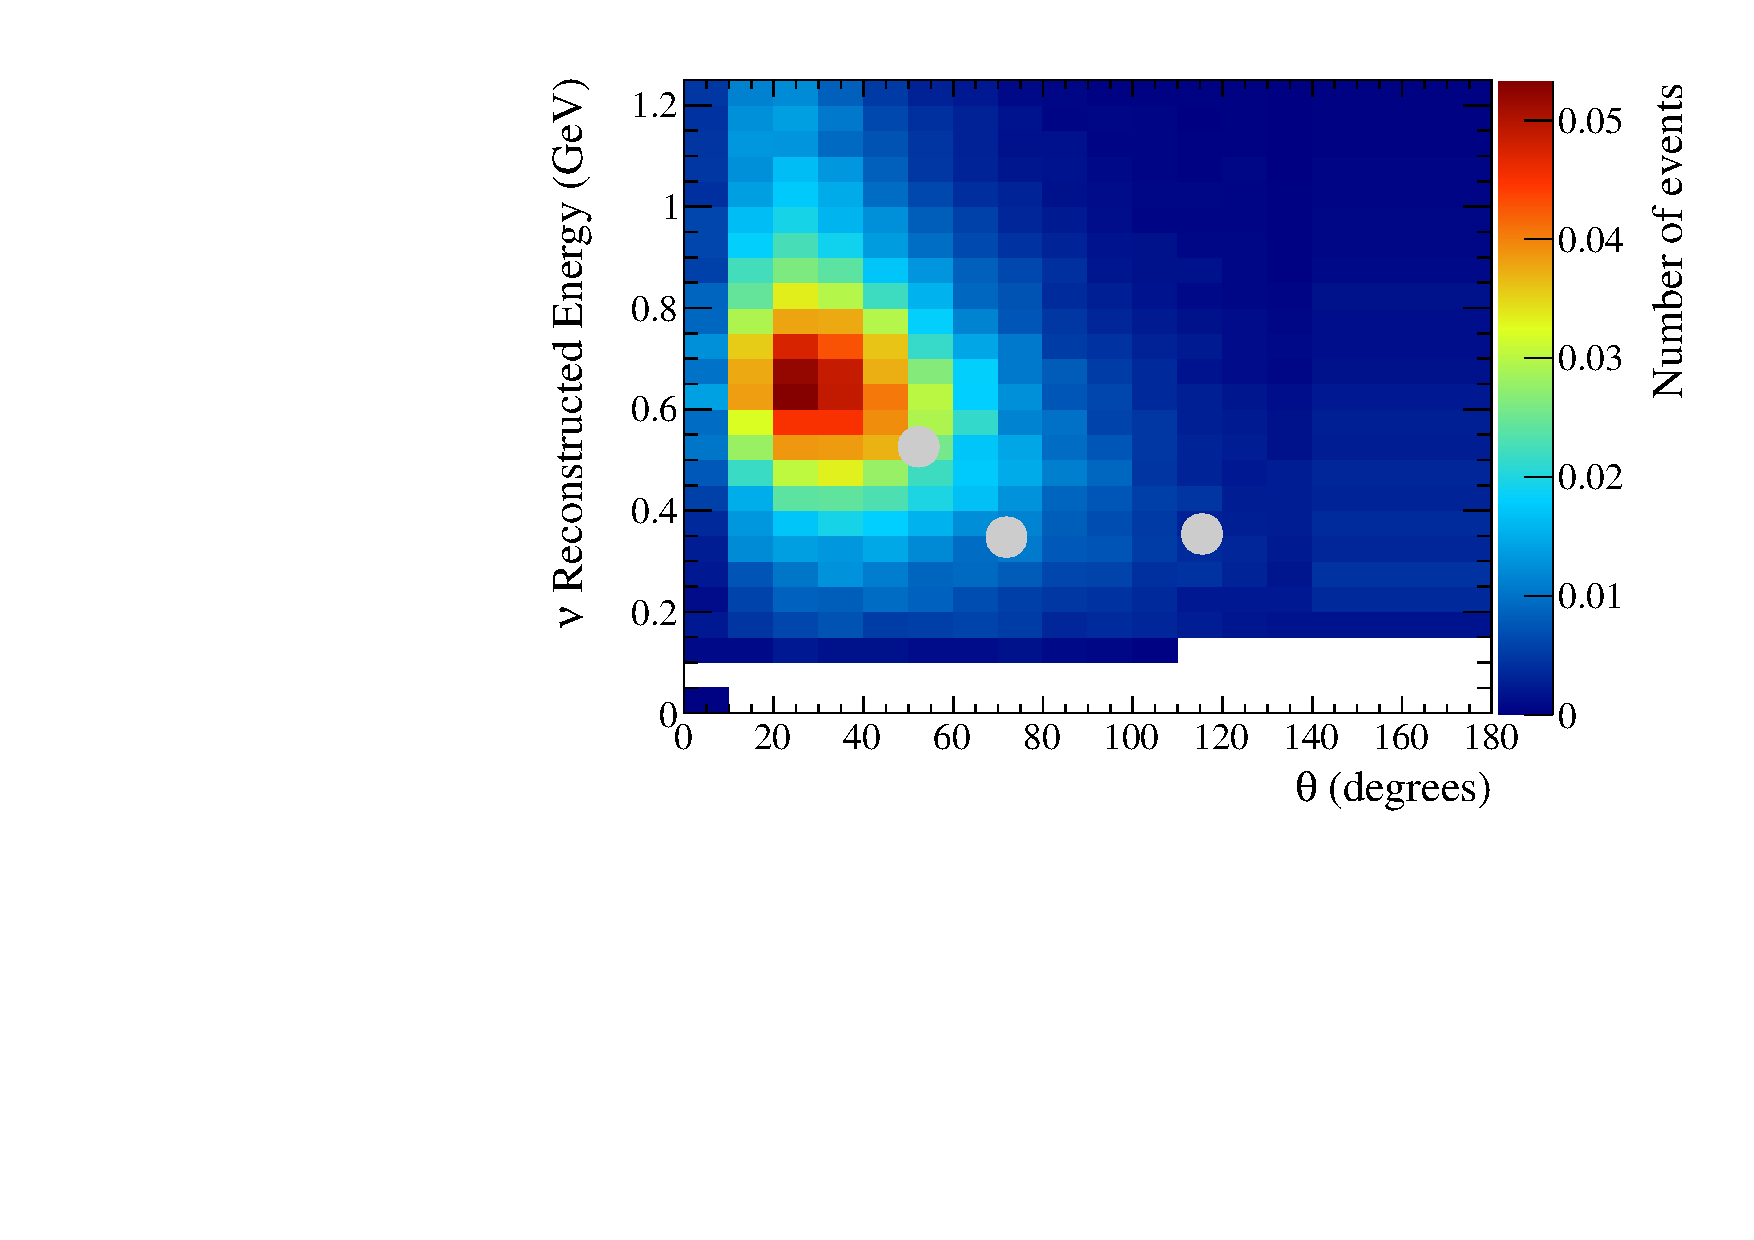
\includegraphics[width=0.9\textwidth]{./joint_plots/data/data_mc_rhc1re_2d_tot.pdf}
\caption{Electron-like, antineutrino mode}
\end{subfigure}
\caption {
%{\large{PREDICTED SPECTRA COMPARED TO DATA}}
The predicted spectra compared to the Run 1-6 dataset (dots),
which corresponds to an exposure 
of \TotalPotNu POT in neutrino mode
and
of \TotalPotNuBar POT in antineutrino mode,
are shown.
The expected distribution corresponds to the oscillation parameters of the Asimov data set A shown in table~\ref{tab:osc_params_joint_asimov}.
The spectra were generated with the systematic parameters measured with the ND280 data 
shown in tab.~\ref{tab:banff_uncertainties_flux_fhc},~\ref{tab:banff_uncertainties_flux_rhc},
~\ref{tab:banff_uncertainties_xsec} and~\ref{tab:banff_uncertainties_skdetfsi}.
}
\label{fig:spectra_expVsdata_asimov_A}
\end{figure}


% Table summarizing the # of observed events in Run 1-6

\begin{table}[htb]
\centering
\begin{tabular}{| c | c | c | c | c | c | c |}
\hline
Beam mode	& Sample		& Exp. Asimov A  	& Exp. Asimov B	& Exp. Not Osc			& Observed 	& Best fit\\
\hline
neutrino	 	& $\mu$-like 	& 125.914			& 130.464 		& 484.737				& 124 		& 125.688 \\
neutrino 		& $e$-like  	& 26.594			& 19.954			& 5.698				& 31 			& 26.969 \\
antineutrino 	& $\mu$-like 	& 34.284			& 35.032			& 99.02				& 34 			& 34.114 \\
antineutrino 	& $e$-like 	& 3.218			& 3.355			& 1.253				& 3 			& 3.344 \\
\hline
\end{tabular}
\caption{
The observed, expected and best-fit number of events in Run 1-6 data set
for an exposure
of \TotalPotNu POT in neutrino mode
and
of \TotalPotNuBar POT in antineutrino mode
are shown 
for each selected sample.
The prediction is produced using the BANFF tuning
and the oscillation parameters shown in Tab.~\ref{tab:osc_params_joint_asimov}.
The total number of events of the best-fit spectra is obtained by using Eq.~\ref{eq:bestfit_spectrum_marg}.
}
\label{tab:num_events}
\end{table}


%--------------------------------------------------------------------------------------
%
% 1-dimensional chisq & best-fit
%
%--------------------------------------------------------------------------------------

\subsection {1-dimensional $\chi^2$ distributions and best-fit}
\label{sec:chisq_1d}


% 1-dimensional contours

The same 1-dimensional $\chi^2$ distributions as in sec.~\ref{sec:sensi} are produced
and shown in Fig.~\ref{fig:joint_data_fit_1d}.
The best-fit value of $\delta_{CP}$ when the reactor constraint is applied is -1.854
not as close to $-\pi/2$ as the Run 1-4 fit result, which best-fit value was -1.601 (see Tab.~\ref{tab:osc_params_joint_asimov}).
However the difference of $\chi^2$ between $\delta_{CP}^{bf}$ (best-fit value) and $\delta_{CP}=-\pi/2$ is smaller than 0.1.
So the result is consistent with $\delta_{CP} = -\pi/2$ as well as the Run 1-4 data fit.
 

Looking at the $\chi^2$ distribution of $\sin^2 \theta_{13}$ with T2K only data
we can see that the reactor measurements are 
in agreement with the T2K data at about $1\sigma$ level if $\delta_{CP} \sim - \pi/2$
and normal hierarchy is assumed.


\begin{figure*}[htb]
\center
\begin{subfigure}[b]{0.49\textwidth}
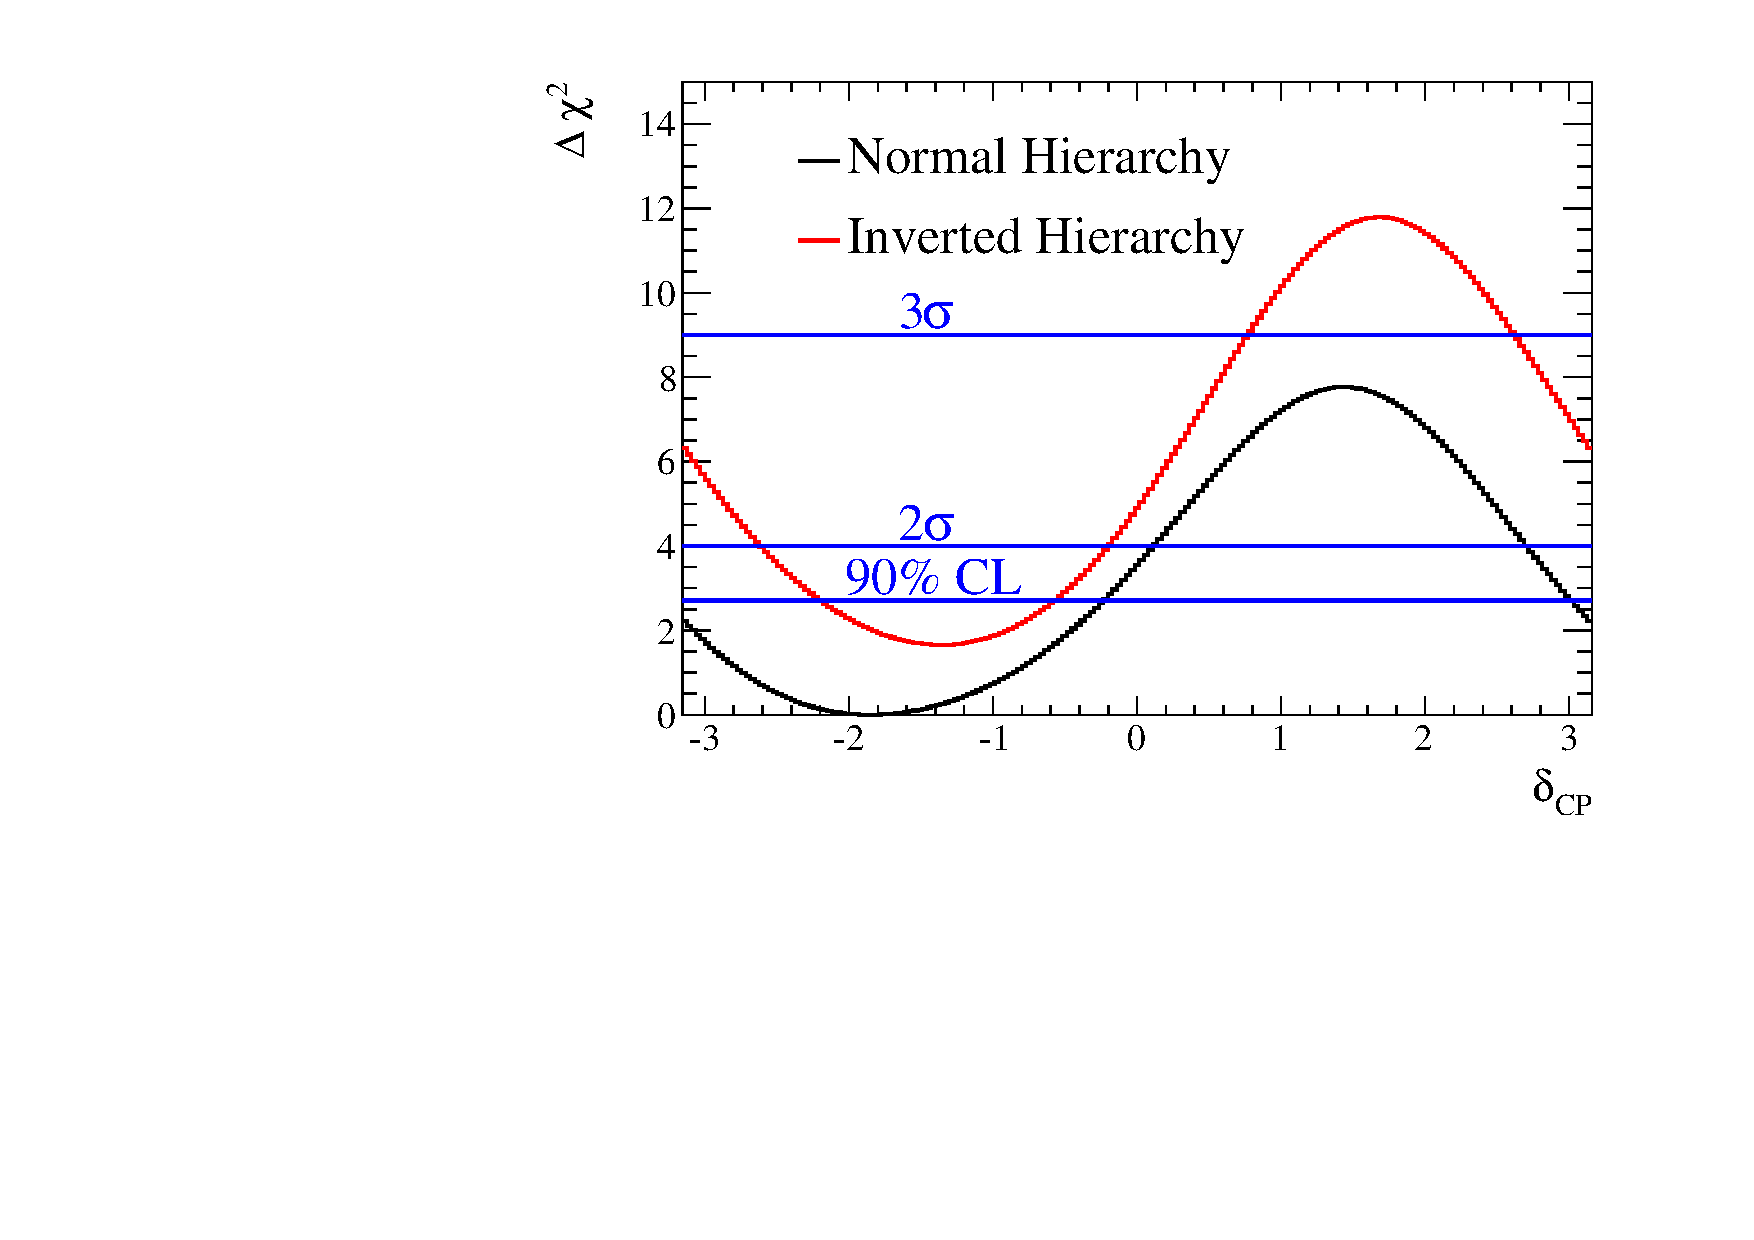
\includegraphics[width=0.9\textwidth]{joint_plots/data_contours/dcp_react_data_constdchisq.pdf}
\caption{$\delta_{CP}$ with reactor constraint}
\label{fig:dcp_fit_with_reactor_data}
\end{subfigure}
\begin{subfigure}[b]{0.49\textwidth}
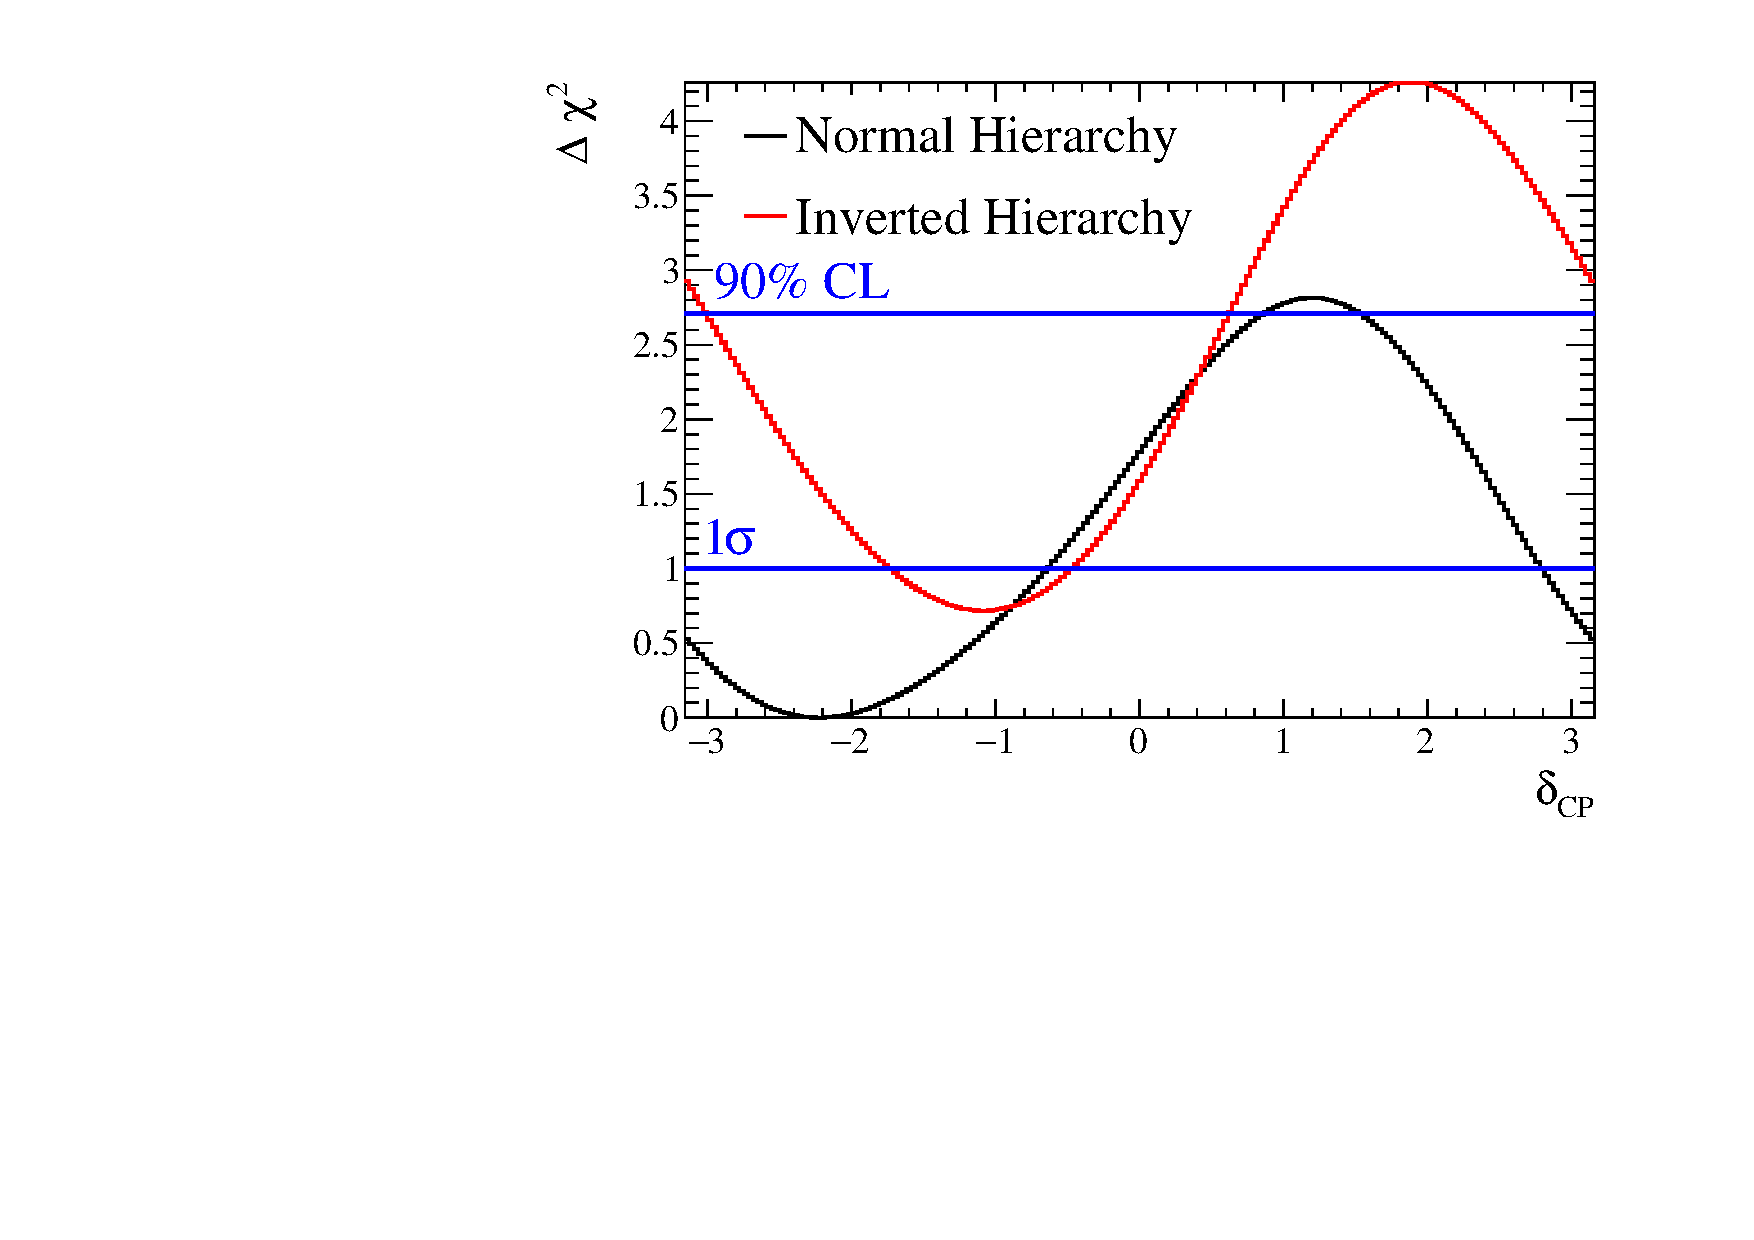
\includegraphics[width=0.9\textwidth]{joint_plots/data_contours/dcp_t2konly_data_constdchisq.pdf}
\caption{$\delta_{CP}$ with T2K data only}
\end{subfigure}
\begin{subfigure}[b]{0.49\textwidth}
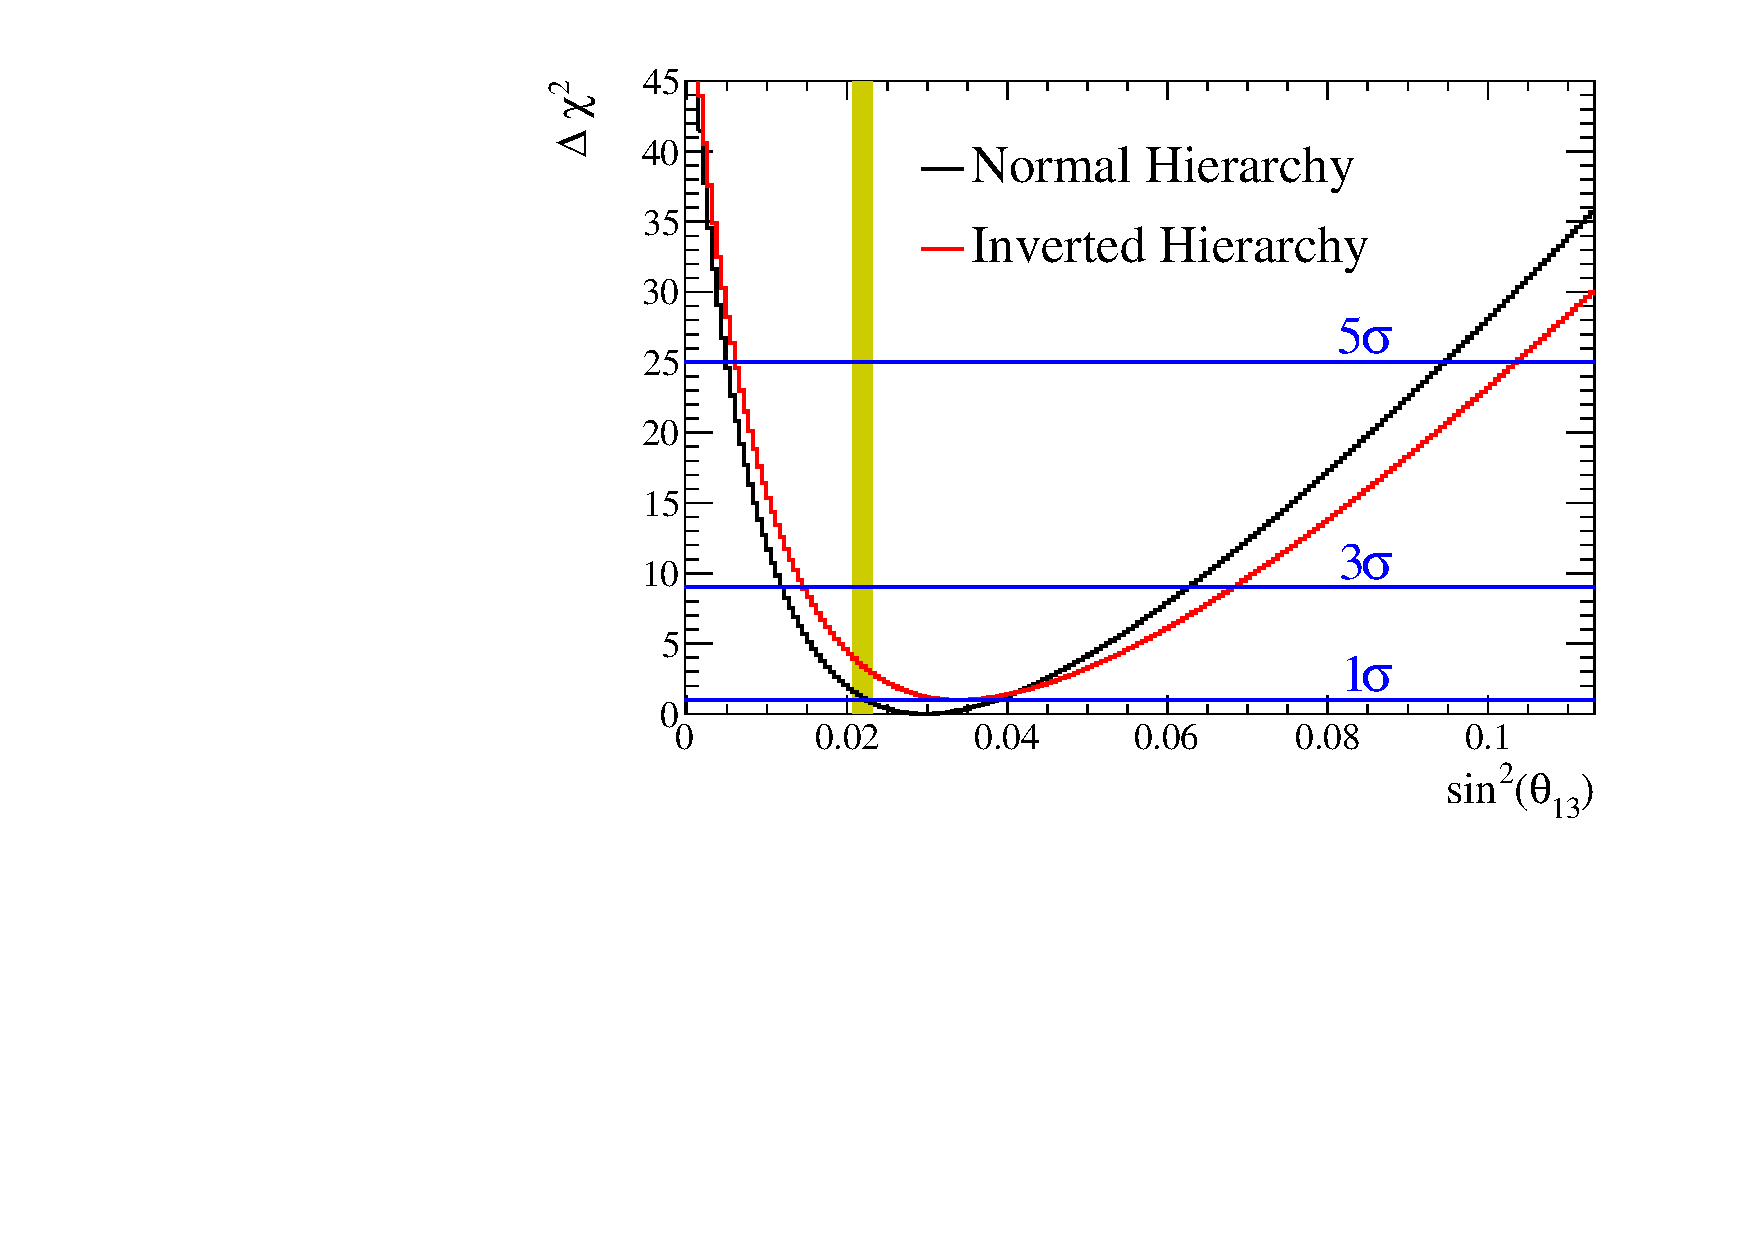
\includegraphics[width=0.9\textwidth]{joint_plots/data_contours/sinsqth13_t2konly_data_constdchisq}
\caption{$\sin^2 \theta_{13}$ with T2K data only}
\end{subfigure}
\begin{subfigure}[b]{0.49\textwidth}
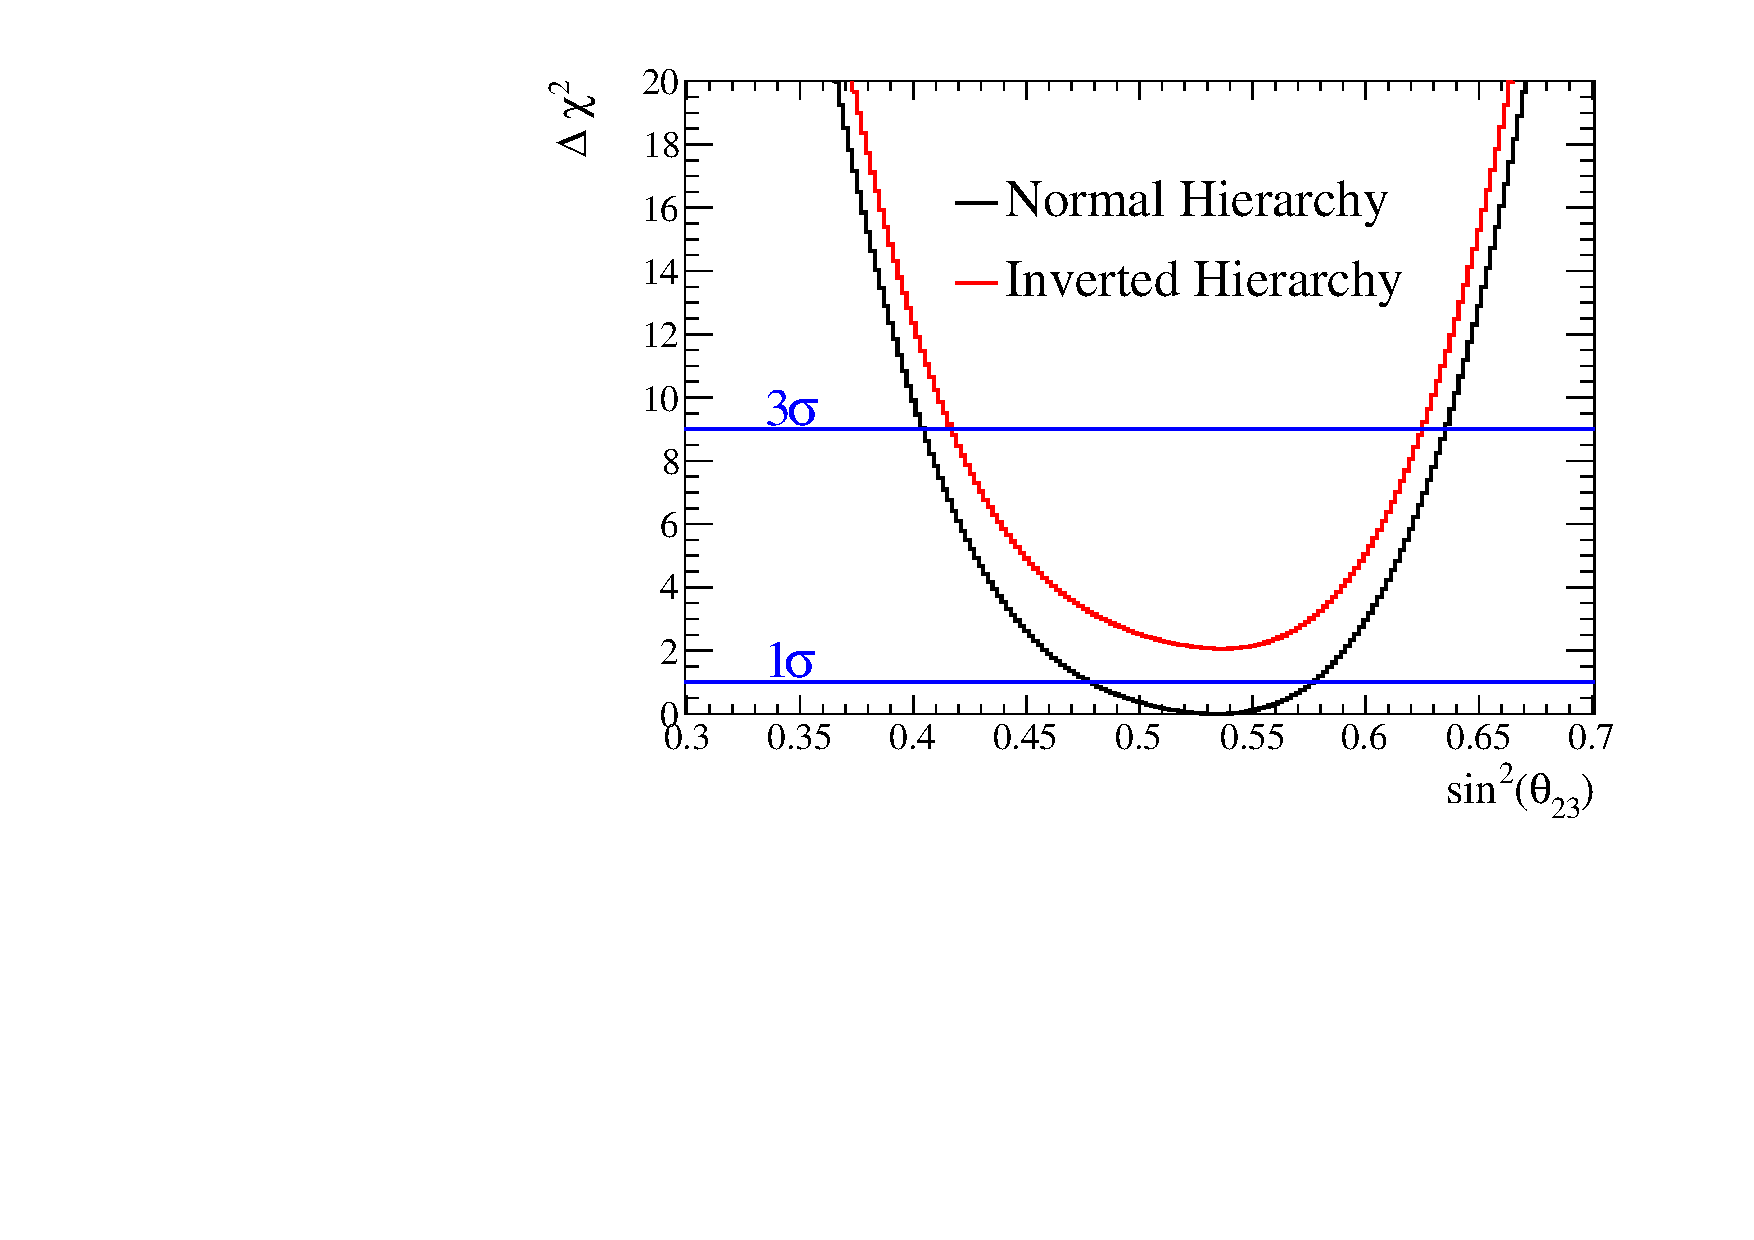
\includegraphics[width=0.9\textwidth]{joint_plots/data_contours/sinsqth23_react_data_constdchisq.pdf}
\caption{$\sin^2 \theta_{23}$ with reactor constraint}
\end{subfigure}
\begin{subfigure}[b]{0.49\textwidth}
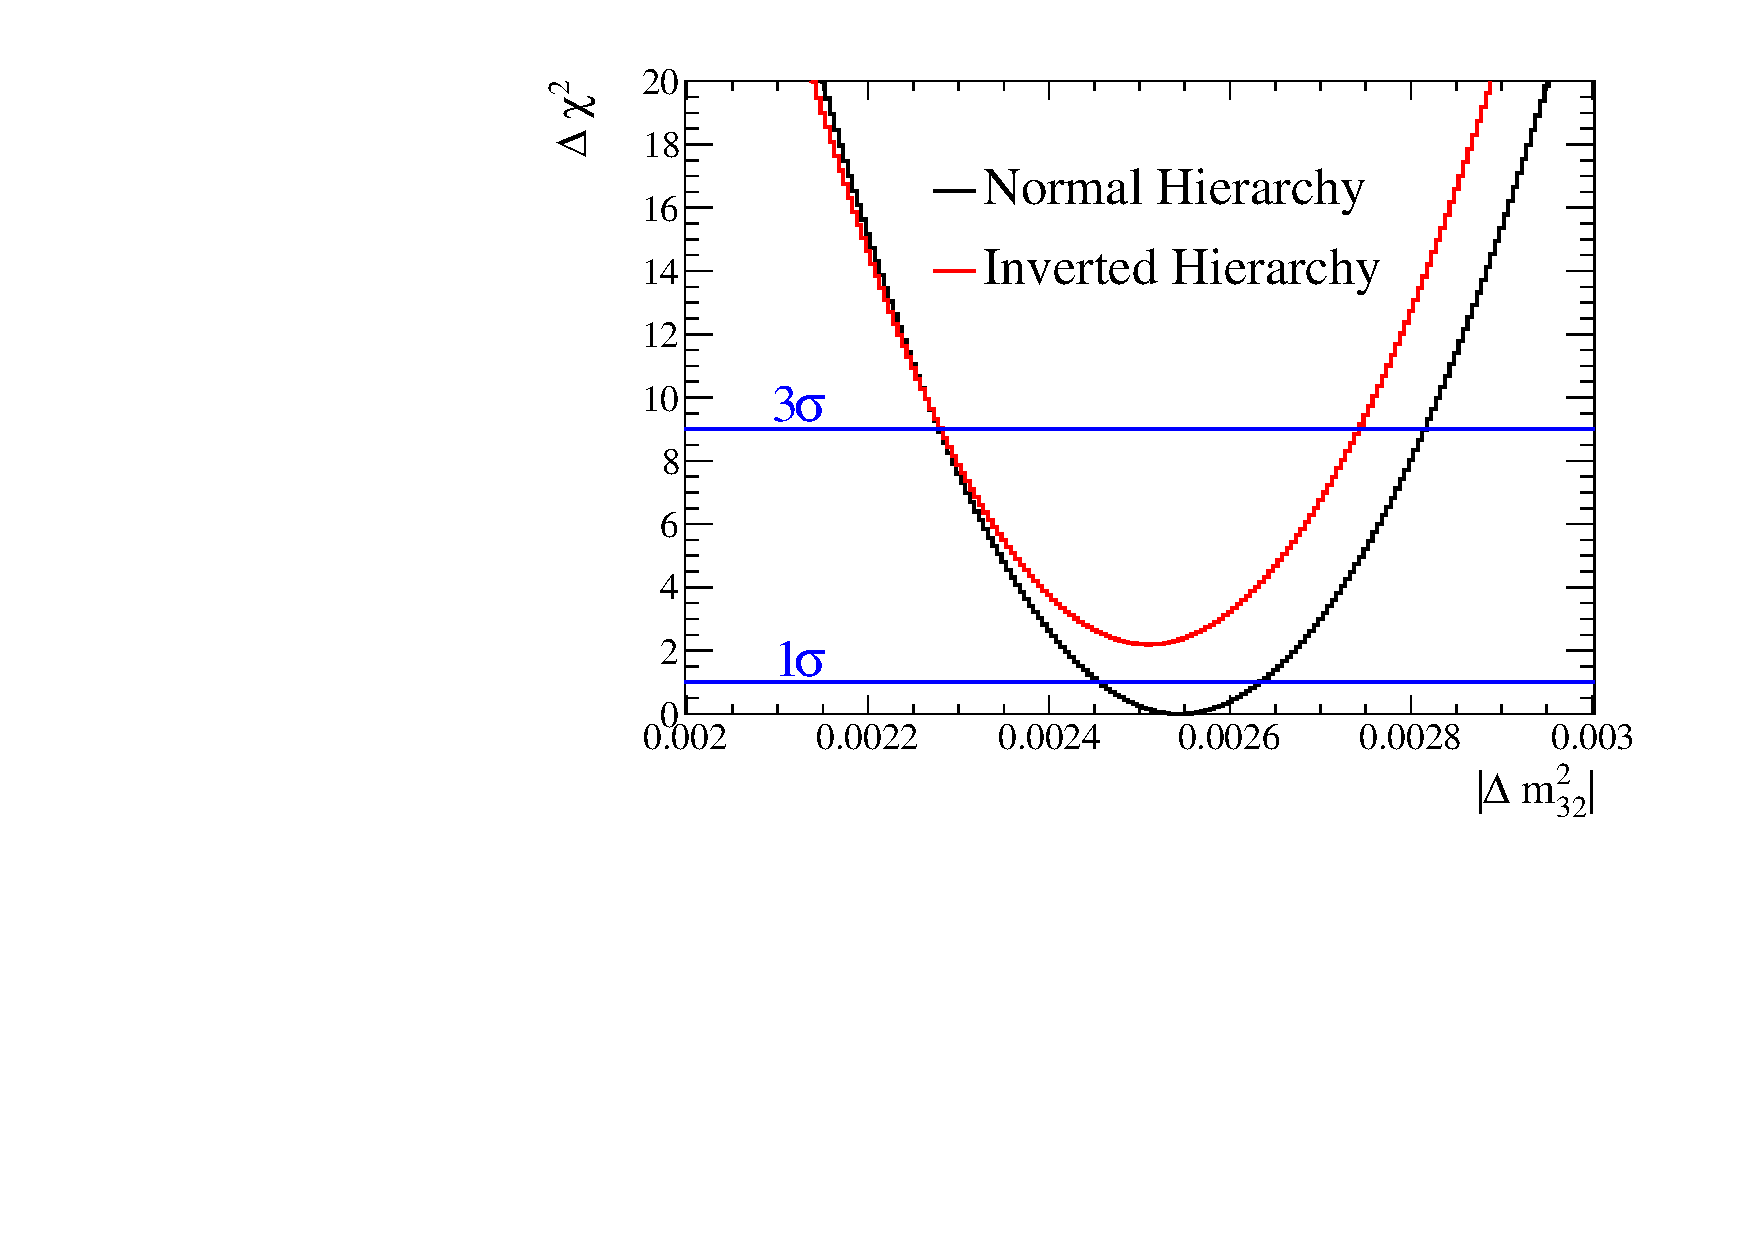
\includegraphics[width=0.9\textwidth]{joint_plots/data_contours/dmsq_react_data_constdchisq.pdf}
\caption{$\Delta m^2_{32}$ ($\Delta m^2_{13}$) with reactor constraint}
\end{subfigure}
\caption{
%    \huge{TO UPDATE} % caption is already ok
%{\large{MEASURED 1D DELTACHISQ DISTRIBUTIONS}}
Measured $\Delta \chi^2$ distributions
with the full run 1-6 data set.
Both normal (black) and inverted (red) hierarchies are shown. 
%Both 68\% (dashed line) and 90\% CL (solid line) are shown.
%For $\delta_{CP}$ confidence intervals are performed using the
%\emph{Feldman-Cousins} method,
%while for the other oscillation parameters
The \emph{constant} $\Delta \chi^2$ method is used. %(see app.~\ref{app:method_cl}).
Both normal and inverted hierarchy $\Delta \chi^2$ distributions are shifted with respect to the same global minimum. 
All the oscillation parameters which are not parameters of interest
are marginalised using the prior distributions shown in tab.~\ref{tab:marg_binnning}.
The measured $\Delta \chi^2$ distribution as a function of $\sin^2 \theta_{13}$ is compared
with the value given by the global analysis of the reactor measurements,
$\sin^2 \theta_{13} = 0.0219 \pm 0.0012 $
\cite{pdg_2014},
shown by the yellow bar.
}
\label{fig:joint_data_fit_1d}
\end{figure*}


%\vspace{3mm}
%{\huge{
%TODO: ADD COMMENTS ABOUT RESULTS
%}}
%\vspace{3mm}


In Fig.~\ref{fig:joint_dcp_nu_nubar}
the $\chi^2$ distributions as a function of $\delta_{CP}$
with reactor constraint
is obtained by 
running the analysis using either only neutrino 
or antineutrino mode samples for the Run 1-6 data set,
in order to check the compatibility of neutrino and antineutrino mode data.
The result is mainly driven by the excess of the observed number
of events in $e$-like neutrino mode sample compared to what is expected.
Though the significance given by the antineutrino mode samples is still low,
also given by the fact that $\sin^2 \theta_{23}$ is not constrained 
by the antineutrino mode $\mu$-like sample
as much as by  
the neutrino mode $\mu$-like sample,
it is interesting to note that the antineutrino data also prefer 
a value of $\delta_{CP}$ close to $-\pi / 2$.

%\vspace{3mm}
%{\huge{
%TODO: ADD COMMENTS ABOUT COMPARISON OF 
%NEUTRINO AND ANTINEUTRINO FIT OF DELTACP
%}}
%\vspace{3mm}

\begin{figure*}[htb]
\center
%
\includegraphics[width=0.9\textwidth]{./images/missing_plot-eps-converted-to.pdf}
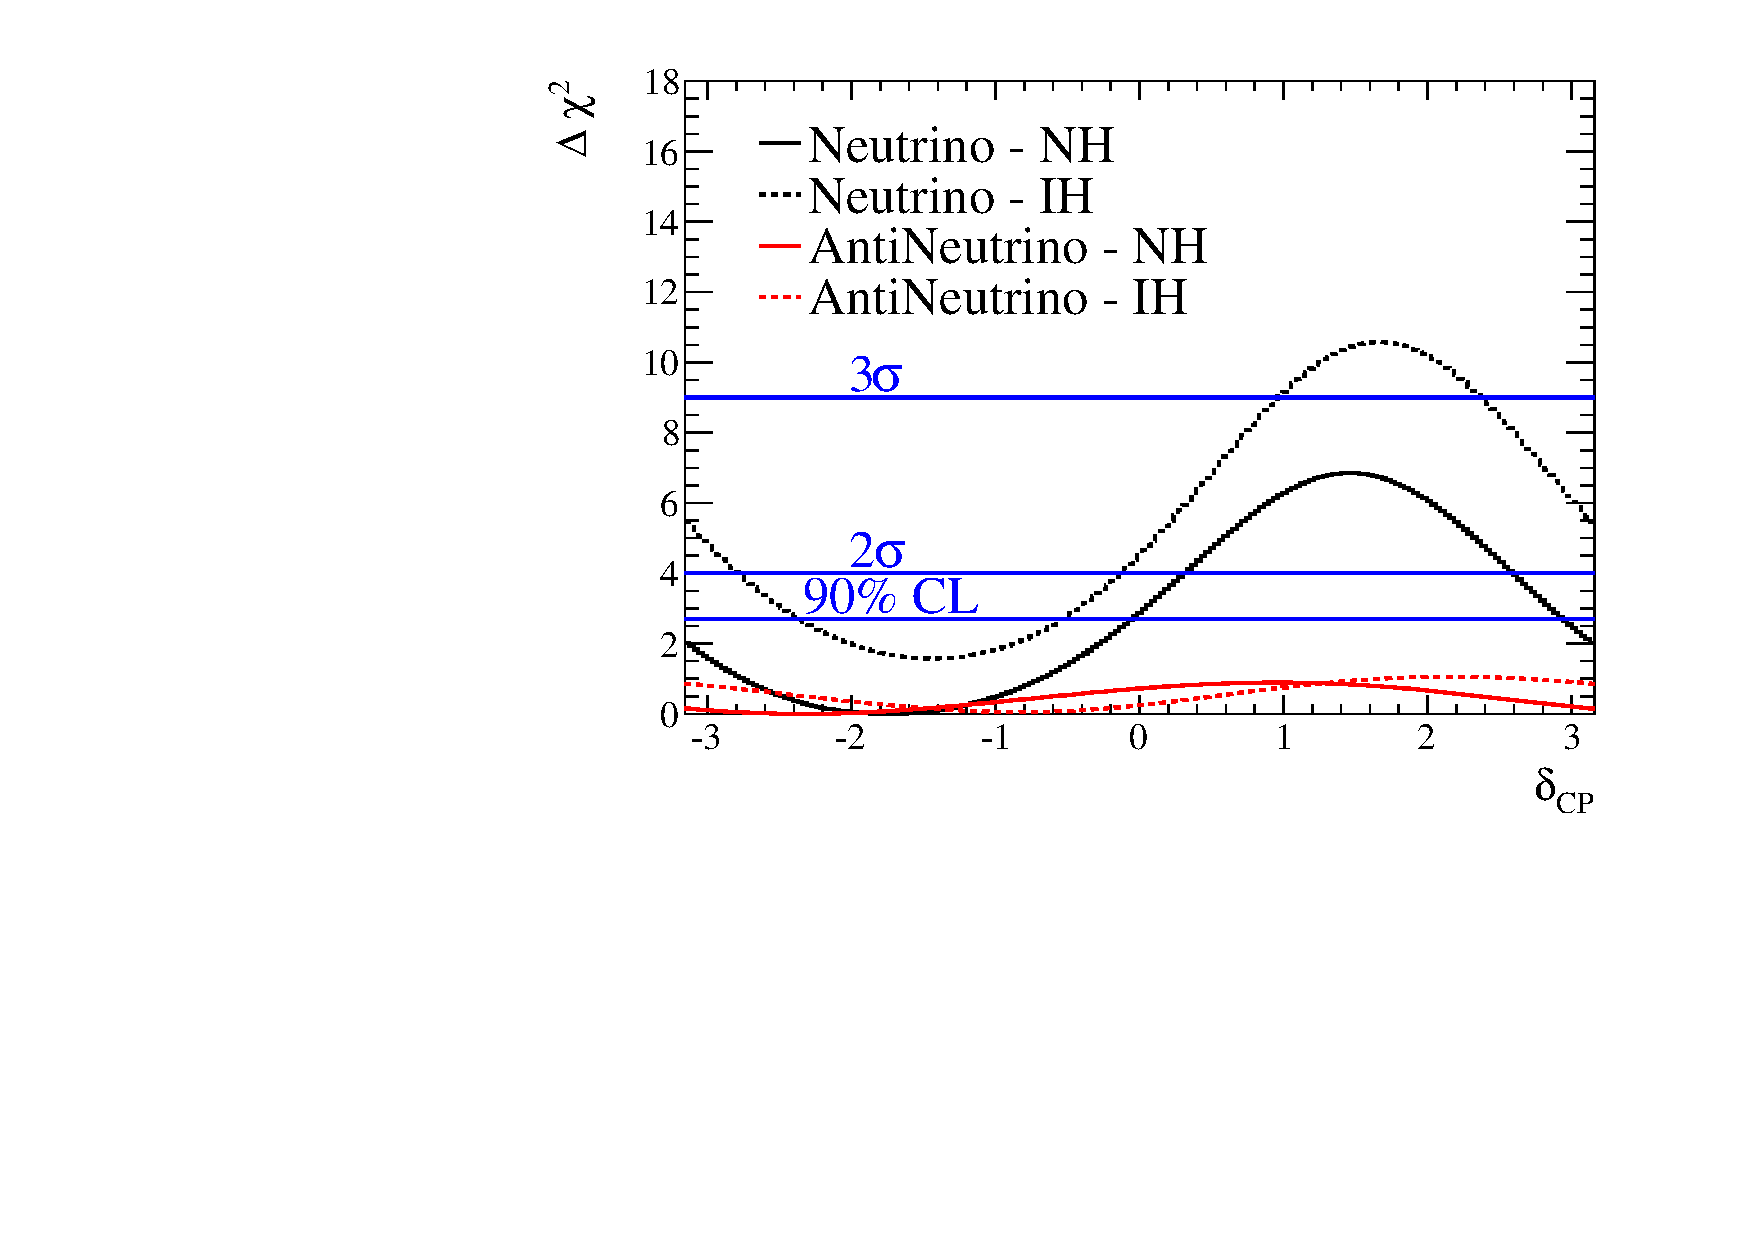
\includegraphics[width=0.5\textwidth]{./joint_plots/data_contours/dcp_react_data_constdchisq_fhcVsrhc.pdf}
\caption{
%{\large{MEASURED 1D DELTACHISQ OF DELTACP FOR 
%NEUTRINO AND ANTINEUTRINO  MODES SEPARATELY}}
Measured $\Delta \chi^2$ distributions
with the full run 1-6 data set
as a function of
$\delta_{CP}$ 
with reactor constraint.
Both normal (black) and inverted (red) hierarchies are shown. 
%Both 68\% (dashed line) and 90\% CL (solid line) are shown.
%For $\delta_{CP}$ confidence intervals are performed using the
%\emph{Feldman-Cousins} method,
%while for the other oscillation parameters
The \emph{constant} $\Delta \chi^2$ method is used. %(see app.~\ref{app:method_cl}).
Both normal and inverted hierarchy $\Delta \chi^2$ distributions are shifted with respect to the same global minimum. 
All the oscillation parameters which are not parameters of interest
are marginalised using the prior distributions shown in tab.~\ref{tab:marg_binnning}.
}
\label{fig:joint_dcp_nu_nubar}
\end{figure*}


In \cref{fig:joint_data_fit_1d_rateonly} the $\chi^2$ distributions as a function of $\delta_{CP}$
is obtained by performing a rate-only analysis; 
instead of using the shape information of the $E_{reco}$ Vs $\theta_l$ spectra,
the total number of events of each sample is fitted, 
reducing the $E_{reco}$ Vs $\theta_l$ template to 1 bin.
Then the best-fit value of $\delta_{CP}$ is -1.602 closer to $-\pi/2$ with respect to the case
where the shape information is used.

\begin{figure*}[htb]
\center
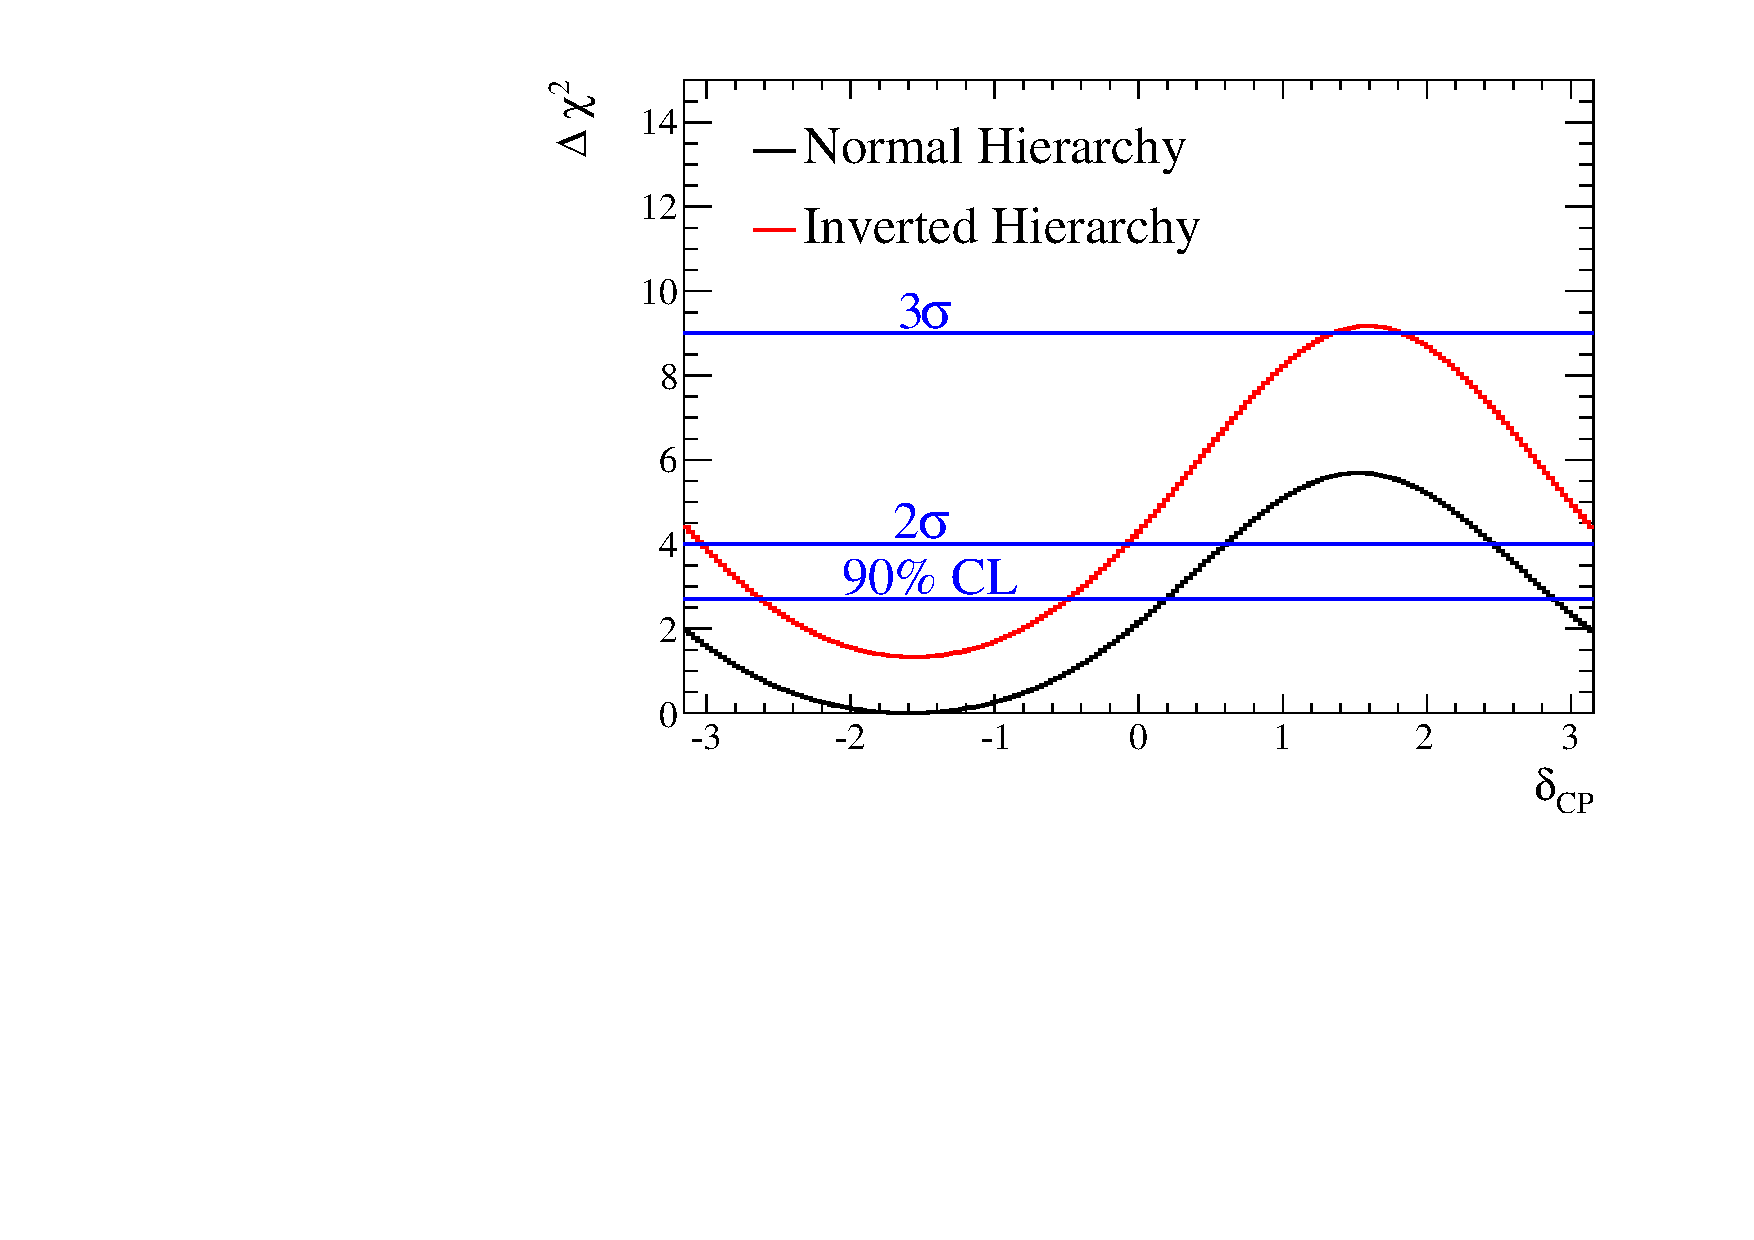
\includegraphics[width=0.5\textwidth]{joint_plots/data_contours/dcp_react_data_constdchisq_rateonly.pdf}
\caption{
%    \huge{TO UPDATE} % caption is already ok
%{\large{MEASURED 1D DELTACHISQ DISTRIBUTIONS}}
Measured $\Delta \chi^2$ distributions
with a rate-only analysis
using the full run 1-6 data set
as a function of
$\delta_{CP}$ 
with reactor constraint.
Both normal (black) and inverted (red) hierarchies are shown. 
%Both 68\% (dashed line) and 90\% CL (solid line) are shown.
%For $\delta_{CP}$ confidence intervals are performed using the
%\emph{Feldman-Cousins} method,
%while for the other oscillation parameters
The \emph{constant} $\Delta \chi^2$ method is used. %(see app.~\ref{app:method_cl}).
Both normal and inverted hierarchy $\Delta \chi^2$ distributions are shifted with respect to the same global minimum. 
All the oscillation parameters which are not parameters of interest
are marginalised using the prior distributions shown in tab.~\ref{tab:marg_binnning}.
}
\label{fig:joint_data_fit_1d_rateonly}
\end{figure*}



In Fig.~\ref{fig:joint_dcp_fc} the confidence intervals obtained with the ``Feldman-Cousins" method
are shown for $\delta_{CP}$ with reactor constraint.
The critical values are calculated as a function of $\delta_{CP}$ as well as the mass hierarchy,
as shown in \cref{sec:cl}.


\begin{figure*}[htb]
\center

\includegraphics[width=0.9\textwidth]{./images/missing_plot-eps-converted-to.pdf}
\caption{
{\large{MEASURED FELDMAN-COUSINS DELTACP W/ REACTORS}}
Measured $\Delta \chi^2$ distributions
with the full run 1-6 data set
as a function of
$\delta_{CP}$ with reactor constraint,
$\delta_{CP}$ with T2K data only,
$\sin^2 \theta_{13}$ with T2K data only,
$\sin^2 \theta_{23}$ with reactor constraint
and
$\Delta m^2_{32}$ ($\Delta m^2_{13}$)
with reactor constraint.
Both normal (black) and inverted (red) hierarchies are shown. 
%Both 68\% (dashed line) and 90\% CL (solid line) are shown.
%For $\delta_{CP}$ confidence intervals are performed using the
%\emph{Feldman-Cousins} method,
%while for the other oscillation parameters
The \emph{constant} $\Delta \chi^2$ method is used. % (see app.~\ref{app:method_cl}).
Both normal and inverted hierarchy $\Delta \chi^2$ distributions are shifted with respect to the same global minimum. 
All the oscillation parameters which are not parameters of interest
are marginalised using the prior distributions shown in tab.~\ref{tab:osc_params_joint_priors}.
The measured $\Delta \chi^2$ distribution as a function of $\sin^2 \theta_{13}$ is compared
with the value given by the global analysis of the reactor measurements,
$\sin^2 \theta_{13} = 0.0219 \pm 0.0012 $
\cite{pdg_2014},
shown by the yellow bar.
}
\label{fig:joint_dcp_fc}
\end{figure*}




% Table of best-fit and 1sigma ranges

In Tab.~\ref{tab:joint_bestfit} the best-fit values as well as the $1\sigma$ ranges for each 
oscillation parameter are shown, for both normal and inverted hierarchy.
The $1\sigma$ ranges are extracted for each oscillation parameter
from the 1-dimensional $\Delta \chi^2$ distributions shown in Fig.~\ref{fig:joint_data_fit_1d},
where one oscillation parameter is free and all the other oscillation as well as the systematic 
parameters are marginalised.
The mass hierarchy is minimized:
for both normal and inverted hierarchy the $1\sigma$ ranges are calculated with respect to the 
same global minimum.
Since this approach is not entirely correct and there does not exist any procedure 
to set more reliable confidence intervals which does not consist of toy MC studies (see \cref{sec:cl_mh}),
the advice to the reader is to give more importance to the difference in $\chi^2_{marg}$
between normal and inverted hierarchies in the respective best-fit points, 
instead of the $1\sigma$ ranges of inverted hierarchy, 
which are smaller by construction.
It is also worth to notice that the $1\sigma$ ranges for normal hierarchy (best-fit)
are set correctly with the constant $\Delta \chi^2$ method in the gaussian approximation.


\begin{table}[htb]
\centering
\begin{tabular}{| c | c | c | c | c || c | c | c | }
\hline
				& {\bf Reactors}		& \multicolumn{3}{c||}{\bf Normal Hierarchy} & \multicolumn{3}{c|}{\bf Inverted Hierarchy} \\
\hline										
\bf Parameter		&				& Best-fit	& $\chi^2_{min}$	& $\pm 1\sigma$ interval  	 	& Best-fit	& $\chi^2_{min}$ 	& $\pm 1\sigma$ interval  \\
\hline
$\delta_{CP}$             & YES      		& -1.854  	& 296.51			& [-2.737; -0.859]			& -1.351	& 298.16			& -	\\
$\delta_{CP}$            & NO        		& -2.231  	& 299.49			& [-$\pi$; -0.640]  \& [2.793;+$\pi$]	& 1.100	& 300.20			& [-1.735;-0.469]			\\
$\sin^2 \theta_{13}$    & NO             	& 0.0299  	& 297.09			& [0.0224; 0.0387]	        		& 0.0339	& 298.09			& -				\\
$\sin^2 \theta_{23}$                      & YES       	& 0.534	& 295.92			& [0.478; 0.577]			& 0.536	& 297.98			& -                 	\\
$\Delta m^2_{32}$ or $\Delta m^2_{13}$  & YES  & 2.545 	& 295.36 			& [2.455; 2.634]			& 2.510 	& 297.56			& -     	\\
($10^{-3} ~\text{eV}^2 / c^4$) 		& YES	& 		&				&						&		&				& \\
\hline
\end{tabular}
\caption{
  %  \huge{TO UPDATE} % caption is already ok
The measured oscillation parameter best-fit
and minimum $\chi^2$ 
values  
as well as the 
$1\sigma$
%68\% 
%and 90\% 
CL intervals are shown,
for both normal and inverted hierarchy. 
The $\pm1\sigma$ interval is obtained by using the 
\emph{constant} $\Delta \chi^2$ method.
All the parameters are measured using the reactor constraint 
$\sin^2 2\theta_{13} = 0.085 \pm 0.005 $
\cite{pdg_2014},
except for $\delta_{CP}$ and $\sin^2 \theta_{13}$.
As explained in \cref{sec:cl_mh}, the gaussian approximation does not work well 
for discrete parameters like the mass hierarchy however, since there is not a clear way
to compute $1\sigma$ ranges for both mass hierarchies without performing
CPU intensive toy MC studies, the constant $\Delta \chi^2$ method is used.
}                                                                                                                                                                                          
\label{tab:joint_bestfit}
\end{table}




% Best-fit spectra

The best-fit spectra, shown in \cref{fig:joint_spectra_bf} are computed as described in sec.~\ref{sec:spectra_bestfit_method}
and are compared to the unoscillated nominal spectra.
For $e$-like samples, where 2-dimensional templates are used,
the projection onto the reconstructed neutrino energy axis is shown.
All the systematic and oscillation parameters are marginalised following the procedure described in sec.~\ref{sec:spectra_bestfit_method},
while $\sin^2\theta_{23}$, $\delta_{CP}$ and the mass hierarchy were fixed to their best-fit values shown in \cref{tab:joint_bestfit}.
Indeed these oscillation parameters have the strongest effect on the measurement,
since $\sin^2\theta_{13}$ is constrained with the reactor measurement.


\begin{figure*}[htb]
\center
\begin{subfigure}[b]{0.49\textwidth}
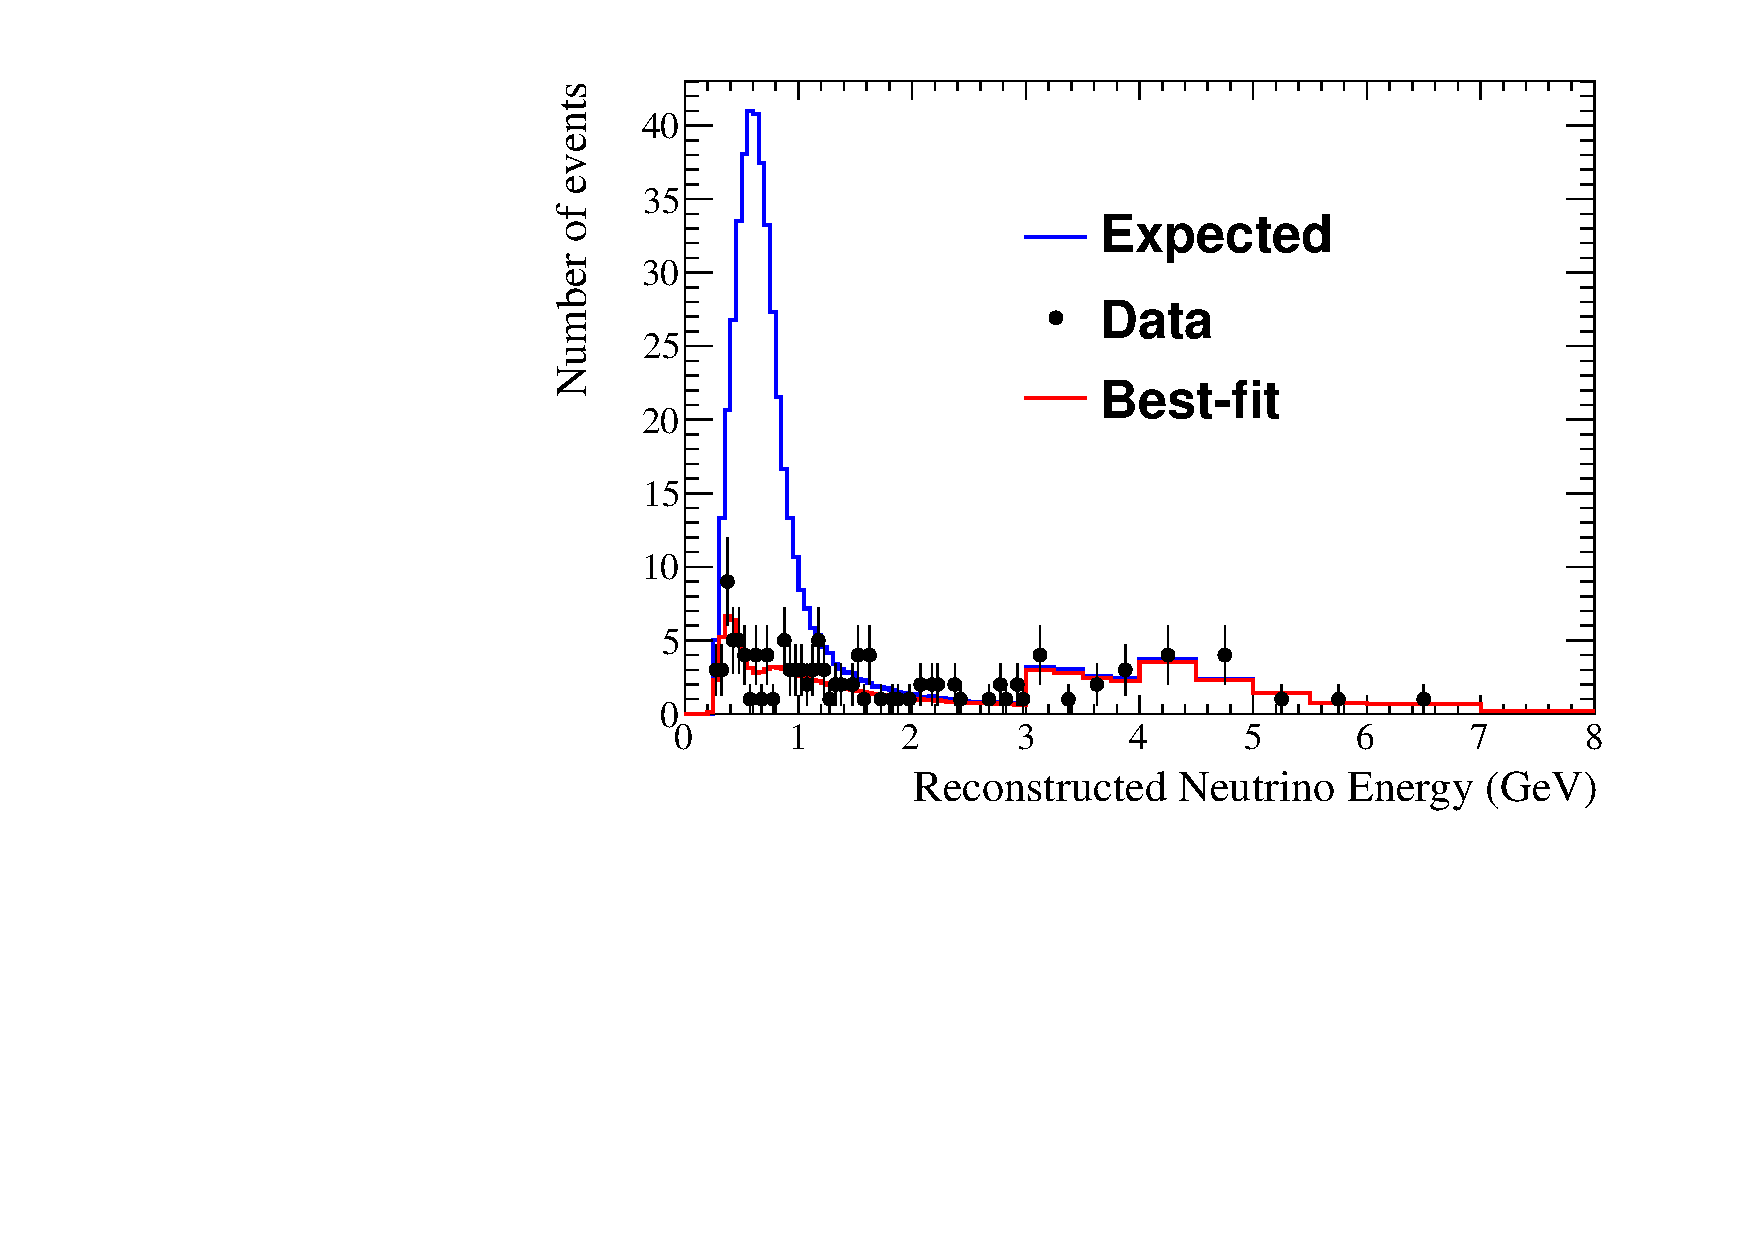
\includegraphics[width=0.9\textwidth]{joint_plots/data/bestfit_marg_sinsqth23Vsdcp_react_1Rmu.pdf}
\caption{Muon-like, neutrino mode}
\end{subfigure}
\begin{subfigure}[b]{0.49\textwidth}
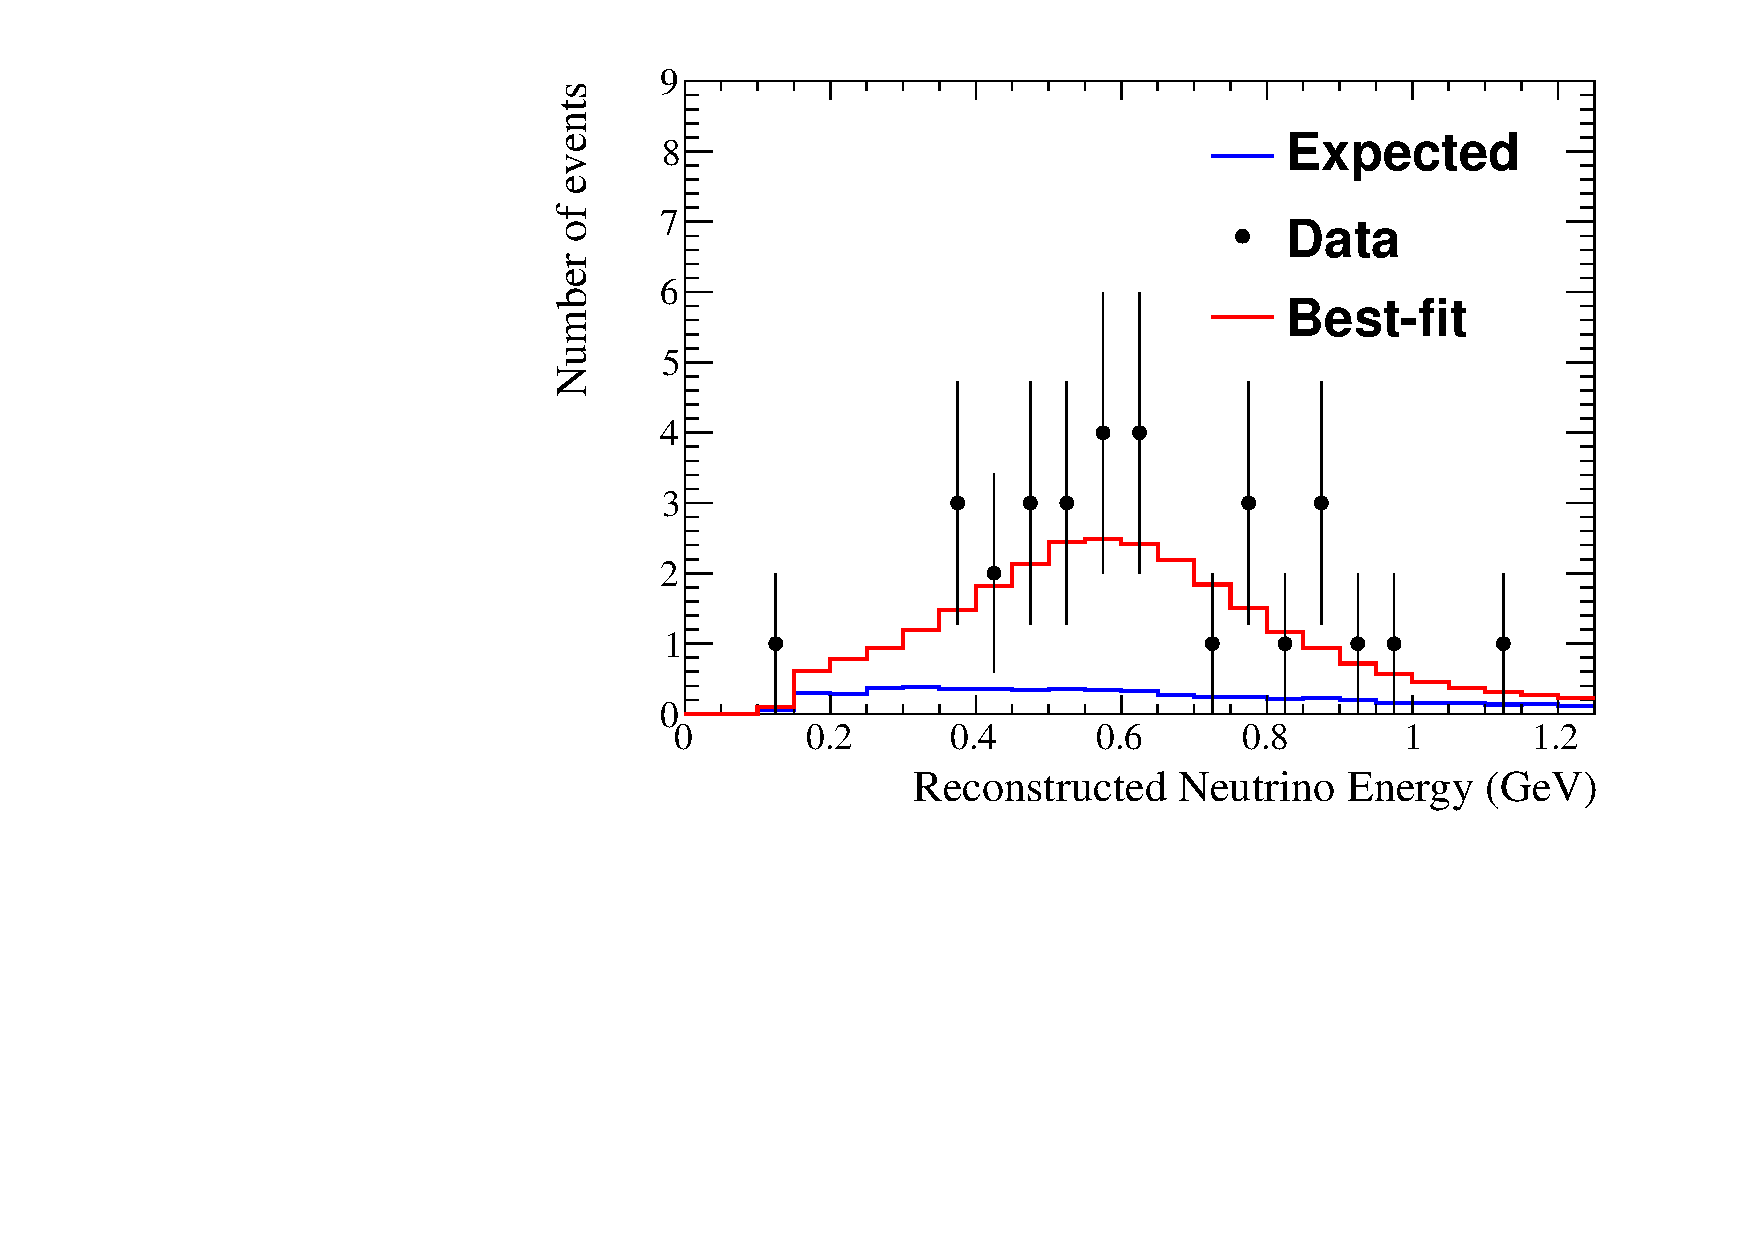
\includegraphics[width=0.9\textwidth]{joint_plots/data/bestfit_marg_sinsqth23Vsdcp_react_1Re.pdf}
\caption{Electron-like, neutrino mode}
\end{subfigure}
\begin{subfigure}[b]{0.49\textwidth}
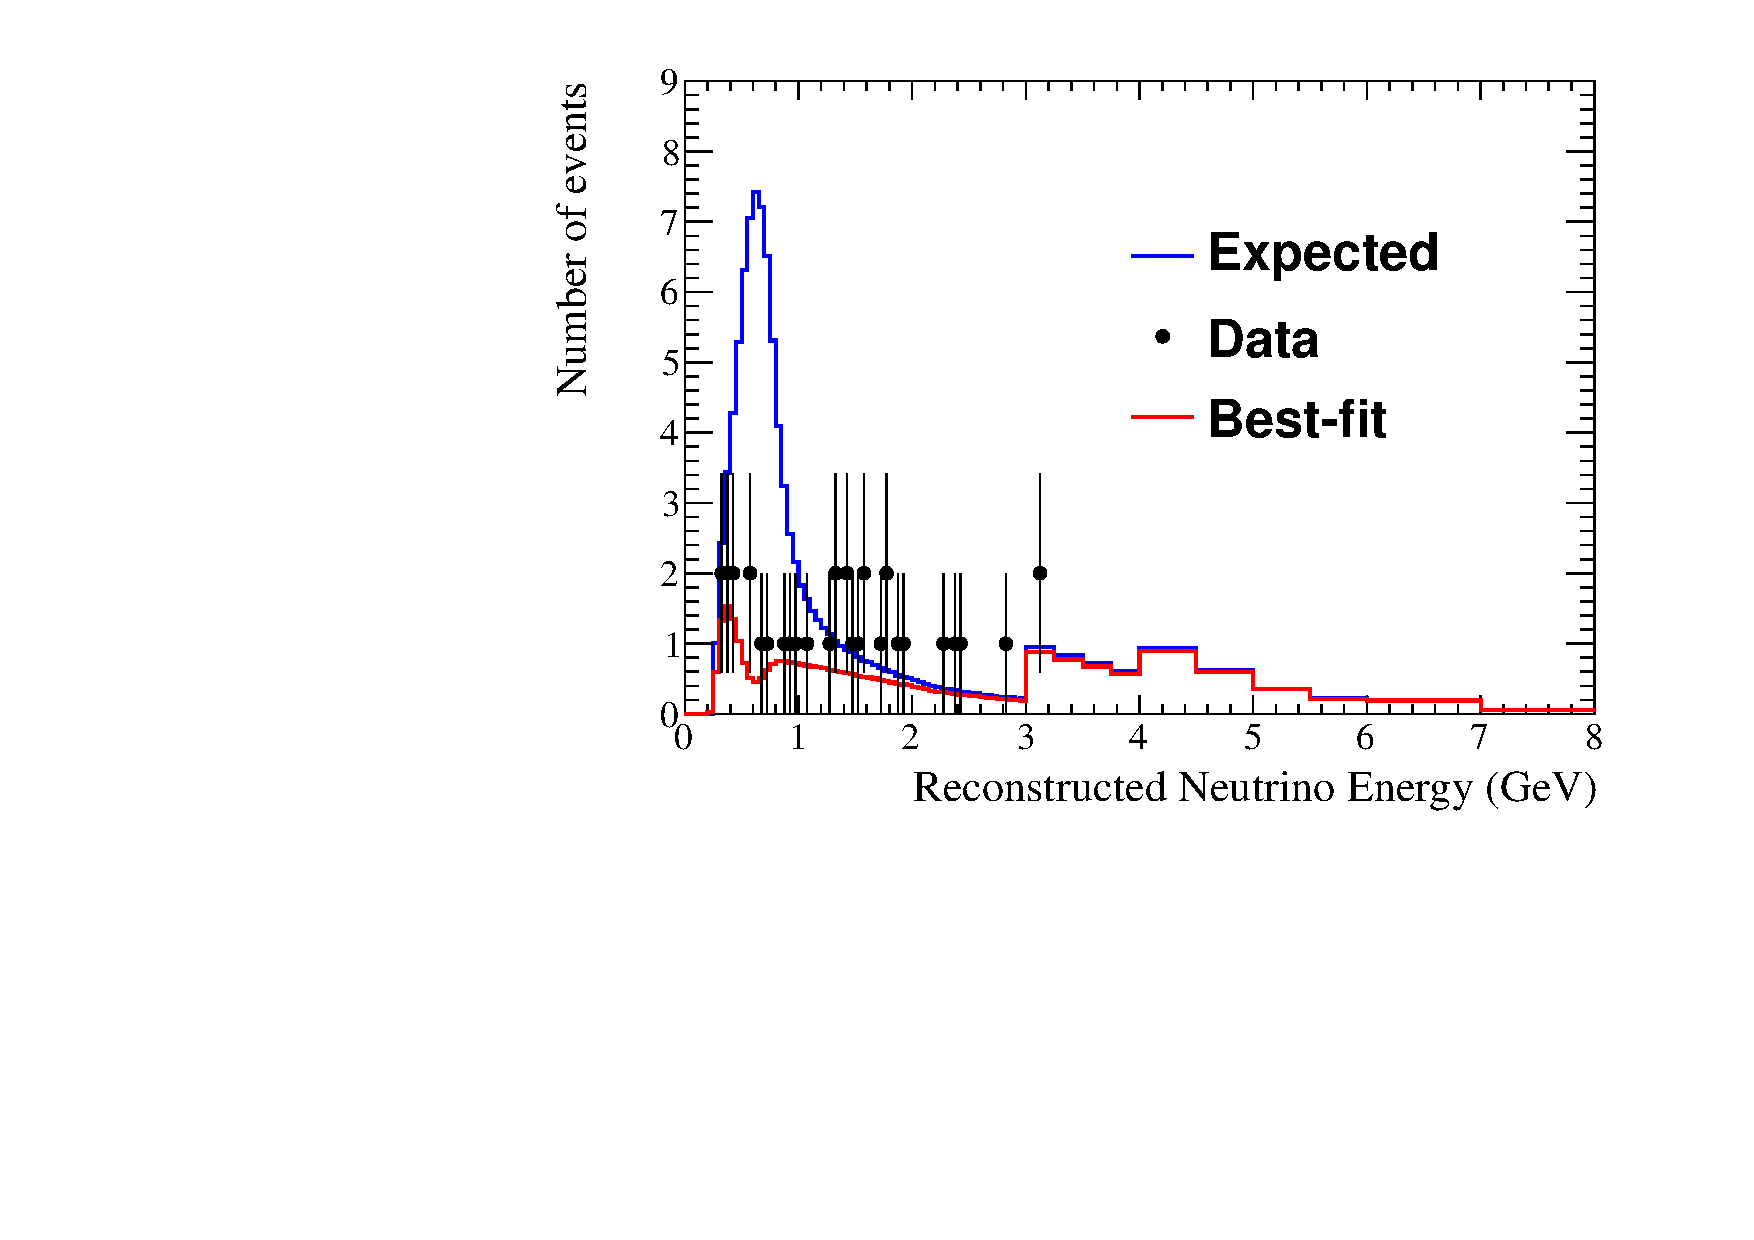
\includegraphics[width=0.9\textwidth]{joint_plots/data/bestfit_marg_sinsqth23Vsdcp_react_RHC1Rmu.pdf}
\caption{Muon-like, antineutrino mode}
\end{subfigure}
\begin{subfigure}[b]{0.49\textwidth}
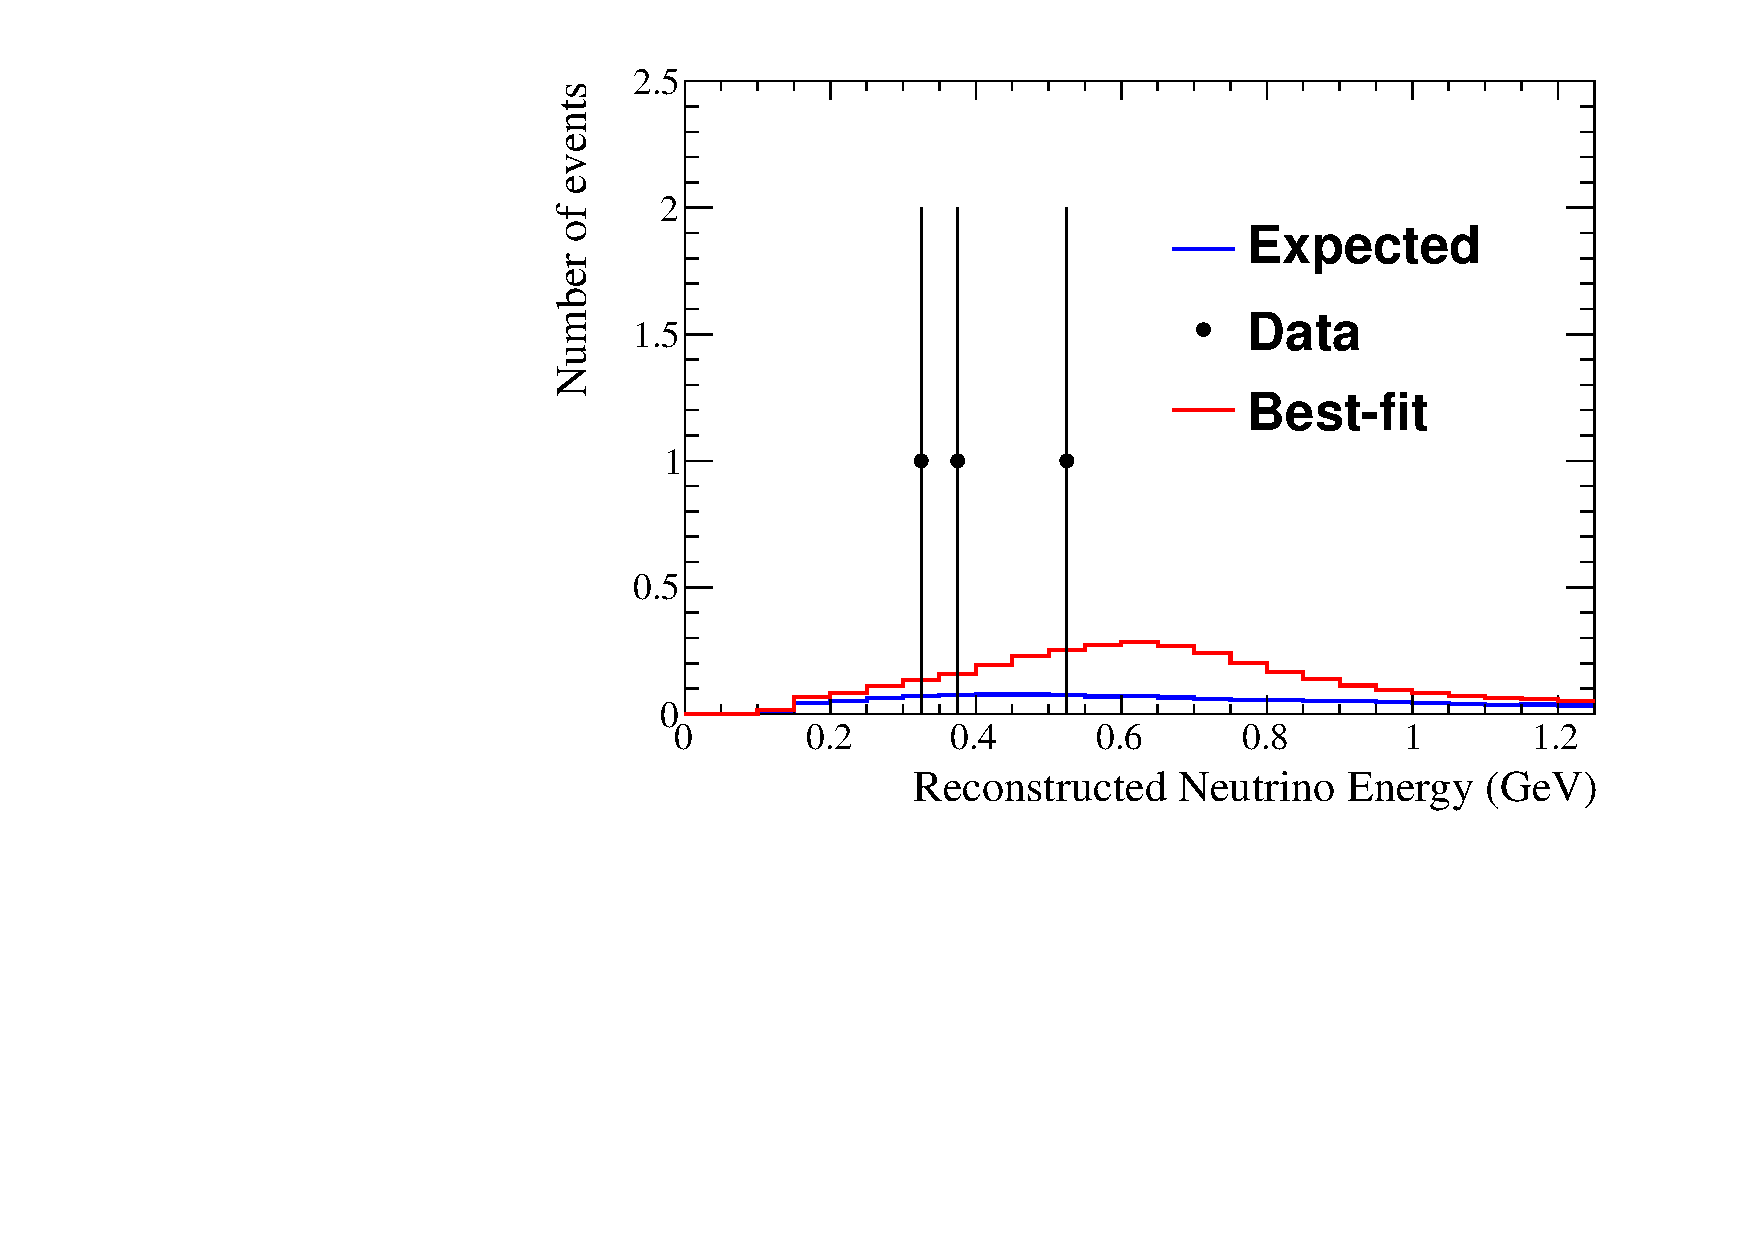
\includegraphics[width=0.9\textwidth]{joint_plots/data/bestfit_marg_sinsqth23Vsdcp_react_RHC1Re.pdf}
\caption{Electron-like, antineutrino mode}
\end{subfigure}
%\includegraphics[width=0.9\textwidth]{joint_plots/data/1rmu_ereco_tot_osc_notosc_bf.pdf}
%\includegraphics[width=0.9\textwidth]{joint_plots/data/rhc1rmu_ereco_tot_osc_notosc_bf.pdf}
%\includegraphics[width=0.9\textwidth]{joint_plots/data/1re_ereco_tot_osc_notosc_bf.pdf}
%\includegraphics[width=0.9\textwidth]{joint_plots/data/rhc1re_ereco_tot_osc_notosc_bf.pdf}
\caption {
%    \huge{TO UPDATE} % caption is already ok
%{\large{MEASURED BEST-FIT ERECO SPECTRA COMPARED TO DATA AND 
%PREDICTED UNOSCILLATED SPECTRA}}
The best-fit spectra as a function of the neutrino reconstructed energy
are shown for each selected sample
of the run 1-6 data set.
They correspond to the fit of 
$\sin^2 \theta_{23}$, $\delta_{CP}$ and mass hierarchy 
with reactor constraint
where all the nuisance parameters are marginalised. 
The method described in sec.~\ref{eq:bestfit_spectrum_marg} is used.
The best-fit distributions are compared with the 
predicted unoscillated spectrum (all the oscillation parameters are set to 0),
generated with the systematic parameters measured with the ND280 data 
shown in tab.~\ref{tab:banff_uncertainties_flux_fhc},
~\ref{tab:banff_uncertainties_flux_rhc},
~\ref{tab:banff_uncertainties_xsec}
and~\ref{tab:banff_uncertainties_skdetfsi}.
}
\label{fig:joint_spectra_bf}
\end{figure*}



% Goodness of fit

A goodness of test fit is performed by comparing data with the best fit spectra shown in \cref{fig:joint_spectra_bf}.
In order to determine how compatible the data is with our model 
the log likelihood is calculated for each sample as in \cref{eq:chisquare}
and the $\chi^2 / ndof$ is used to estimate the fit probability using the Poisson statistic, 
given the number of degrees of freedom equal to $ndof = N_{bins} - N_{free} (8-5 = 3)$,
where $N_{bins}$ is the number of template bins and $N_{free}$ is the number of free parameters in the fit.
The free parameters are $\sin^2 \theta_{23}$, $\delta_{CP}$ and the mass hierarchy in this case. 
In this analysis, a coarse binning scheme is used for the goodness of fit test as in previous analyses. 
This is used so that there are enough events in each bin to calculate p-values in the gaussian approximation. 
5 bins (0-0.4, 0.4-0.7, 0.7-1.0, 1.0-2.0 and 2.0-30.0 GeV) are used for the neutrino mode muon-like spectrum, 
1 bin is used for each of the muon-like antineutrino and electron-like spectra
in order to enter the gaussian regime, where the $\chi^2$ distribution is well defined.
The $\chi^2$ and resulting p-value for each spectrum is shown in Tab.~\ref{tab:goodness_of_fit}. 
We see for all the spectra, the data and best fit spectra are very compatible.

\begin{table}[htb]
\centering
\begin{tabular}{| c | c | c |}
\hline
 			& $\chi^2$ / ndf        		& p-value \\ \hline
MH fixed 		& 2.08917 / 6                  	& 0.84	\\ \hline
MH fitted 		& 2.08917 / 5                  	& 0.91	\\ \hline

\end{tabular}
\caption{
Goodness of fit for the 2-dimensional fit of $\sin^2 \theta_{23}$, $\delta_{CP}$ and mass hierarchy 
(both fitted and fixed)
where all the other parameters are marginalised. 
}
\label{tab:goodness_of_fit}
\end{table}

%\begin{table}[htb]
%\centering
%\begin{tabular}{| c | c | c | }
%\hline
%Sample		&  $\chi^2$ / ndf        			& p-value \\ \hline
%muon-like neutrino & 1.47751/ 2                  	&		0	\\ \hline
%muon-like antineutrino & 0.000378452 / 2   	&		0 \\	 \hline
%electron-like neutrino & 0.574525 / 2  		&		0 \\	\hline
%electron-like antineutrino & 0.0367553 / 2	&		0 \\		\hline
%\end{tabular}
%\caption{
%Goodness of fit for each sample spectrum from Sec.~\ref{sec:best_fit_spectra}. 
%}
%\label{tab:goodness_of_fit}
%\end{table}








%--------------------------------------------------------------------------------------
%
% Contours
%
%--------------------------------------------------------------------------------------

\subsection {2-dimensional confidence intervals}
\label{sec:results_bestfit}

The same 2-dimensional confidence intervals as in sec.~\ref{sec:sensi} are produced.
%In Fig.~\ref{fig:joint_chisq_t2krun14bf_2d_nh} and~\ref{fig:joint_chisq_t2krun14bf_2d_ih} the 2-dimensional $\chi^2$ distributions 
%obtained by the fit of the Run 1-6 data set are shown for both normal and inverted hierarchy.
In Fig.~\ref{fig:joint_sensi_t2krun14bf_2d} the corresponding 2-dimensional contours produced
with the Run 1-6 data set are shown drawing the normal and inverted hierarchy contours independently,
i.e. each contour is produced with respect to the global minimum under that hierarchy hypothesis.
In Fig.~\ref{fig:joint_sensi_t2krun14bf_2d_glob} both normal and inverted hierarchy contours
are produced with respect to the same global minimum, i.e. the normal hierarchy hypothesis.

As already explained in \cref{sec:cl_mh}, ``global" and ``independent" contours correspond
respectively to the least and most conservative approach.

As in 1-dimensional analysis results,
looking at contours of $\sin^2 \theta_{13}$ Vs $\delta_{CP}$ with T2K only data, 
in Fig~\ref{fig:ss13_dcp_t2k_only_data_fit}, it is clear that the reactor measurements are 
in agreement with the T2K data at $1\sigma$ level if $\delta_{CP} \sim - \frac{\pi}{2}$. The tension 
between the $\sin^2 \theta_{13}$ reactor constraint and the T2K data constraint is clear at 
$\sim \frac{+\pi}{2}$ where the T2K data prefer a lager mixing angle with both hierarchy hypotheses.
This is the cause of the closed 90\% contour in Fig~\ref{fig:ss13_dcp_with_reactor_data_fit} which is also in good agreement with the 1D $\delta_{CP}$ fit in Fig.\ref{fig:dcp_fit_with_reactor_data}. This effect is much greater for the inverted hierarchy fits and thus leads to a much tighter constraint on $\delta_{CP}$. 
As a result, we see that all $\delta_{CP}$ constraints in 
Fig.~\ref{fig:ss13_dcp_with_reactor_data_fit},~\ref{fig:dmsq_dcp_with_reactor_data_fit},~\ref{fig:ss23_dcp_with_reactor_data_fit} 
are tighter for the inverted hierarchy hypothesis than for the normal.
Fig~\ref{fig:dmsq_dcp_with_reactor_data_fit} also shows a slight anti-correlation between $\delta_{CP}$ 
and $\Delta m^2_{32}$ in the normal hierarchy fit and a correlation in the inverted most likely coming 
from the fact that $\Delta m^2_{32}$ and $cos(\delta_{CP})$ have similar effects on the shape of the appearance spectra. 
In Fig~\ref{fig:ss23_dcp_with_reactor_data_fit} we see correlation where the constraint on $\delta_{CP}$ is narrower 
for smaller values of $\sin^2 \theta_{23}$ as they both appear in the appearance term. 
In Fig~\ref{fig:ss23_dmsq_with_reactor_data_fit} we see that $\sin^2 \theta_{23}$ and $\Delta m^2_{32}$ 
are not very correlated however the inverted hierarchy contour is shifted down in $\Delta m^2_{32}$ 
with respect to the normal hierarchy contour. 
This effect is due to the correlation between $\Delta m^2_{32}$ and the mass hierarchy shown in Fig.~\ref{fig:mass_hierarchy_MC_shift}. 
Indeed the inverted hierarchy hypothesis produces an event migration toward higher energy 
which is balanced in the fit by a lower fit value of $\Delta m^2_{13}$ with respect to the normal hierarchy case.

%This effect is likely due to the correlations between the hierarchy and $\delta_{CP}$ which we see in Fig.~\ref{fig:ss13_dcp_with_reactor_data_fit}, where inverted hierarchy fit excludes $cos(\delta_{CP})=-1$ to a greater significance than the normal hierarchy fit, and $\Delta m^2_{32}$ and $\delta_{CP}$ in Fig.~\ref{fig:dmsq_dcp_with_reactor_data_fit}. 

The \emph{constant} $\Delta \chi^2$ contours with respect to the global minimum in Fig.~\ref{fig:joint_sensi_t2krun14bf_2d_glob} show similar trends. 
As the normal hierarchy was preferred in all fits, the normal hierarchy contours are identical to those in Fig.~\ref{fig:joint_sensi_t2krun14bf_2d}. 
The inverted hierarchy contours are noticeably tighter in all cases. 
In Fig~\ref{fig:ss13_dcp_t2k_only_data_fit_global} we see that there is a closed $\Delta \chi^2=4.61$ contour, 
and in all others the $\Delta \chi^2=4.61$ contour is of similar size to the $\Delta \chi^2=2.3$ contour for the normal hierarchy. 

%\begin{figure*}[htb]
%\center
%
\includegraphics[width=0.9\textwidth]{./images/missing_plot-eps-converted-to.pdf}
%
\includegraphics[width=0.9\textwidth]{./images/missing_plot-eps-converted-to.pdf}
%
\includegraphics[width=0.9\textwidth]{./images/missing_plot-eps-converted-to.pdf}
%\caption{
%{\large{MEASURED 2D CHISQ DISTRIBUTIONS FOR NORMAL HIERARCHY}}
%$\chi^2$ distributions measured  
%with the full run 1-6 data set.
%Normal hierarchy is shown. 
%From top left to bottom right the following combinations of oscillation parameters are shown:
%$\sin^2 \theta_{13}$ Vs $\delta_{CP}$ with T2K data only,
%$\sin^2 \theta_{13}$ Vs $\delta_{CP}$ with reactor constraint
%and
%$\sin^2 \theta_{23}$ Vs $\Delta m^2_{32}$ ($\Delta m^2_{13}$)
%with reactor constraint.
%All the oscillation parameters which are not parameters of interest
%are marginalised using the prior distributions shown in tab.~\ref{tab:osc_params_joint}.
%The $\chi^2$ distribution of $\sin^2 \theta_{13}$ Vs $\delta_{CP}$ without reactor constraint
%is compared with the measurement performed by the reactor experiments, 
%$\sin^2 \theta_{13} = 0.0219 \pm 0.0012 $
%\cite{pdg_2014},
%shown by the yellow bar.
%}
%\label{fig:joint_chisq_t2krun14bf_2d_nh}
%\end{figure*}
%
%\begin{figure*}[htb]
%\center
%
\includegraphics[width=0.9\textwidth]{./images/missing_plot-eps-converted-to.pdf}
%
\includegraphics[width=0.9\textwidth]{./images/missing_plot-eps-converted-to.pdf}
%
\includegraphics[width=0.9\textwidth]{./images/missing_plot-eps-converted-to.pdf}
%\caption{
%{\large{MEASURED 2D CHISQ DISTRIBUTIONS FOR INVERTED HIERARCHY}}
%$\chi^2$ distributions measured  
%with the full run 1-6 data set.
%Inverted hierarchy is shown. 
%From top left to bottom right the following combinations of oscillation parameters are shown:
%$\sin^2 \theta_{13}$ Vs $\delta_{CP}$ with T2K data only,
%$\sin^2 \theta_{13}$ Vs $\delta_{CP}$ with reactor constraint
%and
%$\sin^2 \theta_{23}$ Vs $\Delta m^2_{32}$ ($\Delta m^2_{13}$)
%with reactor constraint.
%All the oscillation parameters which are not parameters of interest
%are marginalised using the prior distributions shown in tab.~\ref{tab:osc_params_joint}.
%The $\chi^2$ distribution of $\sin^2 \theta_{13}$ Vs $\delta_{CP}$ without reactor constraint
%is compared with the measurement performed by the reactor experiments, 
%$\sin^2 \theta_{13} = 0.0219 \pm 0.0012 $
%\cite{pdg_2014},
%shown by the yellow bar.
%}
%\label{fig:joint_chisq_t2krun14bf_2d_ih}
%\end{figure*}

\begin{figure*}[htb]
\center
\begin{subfigure}[b]{0.49\textwidth}
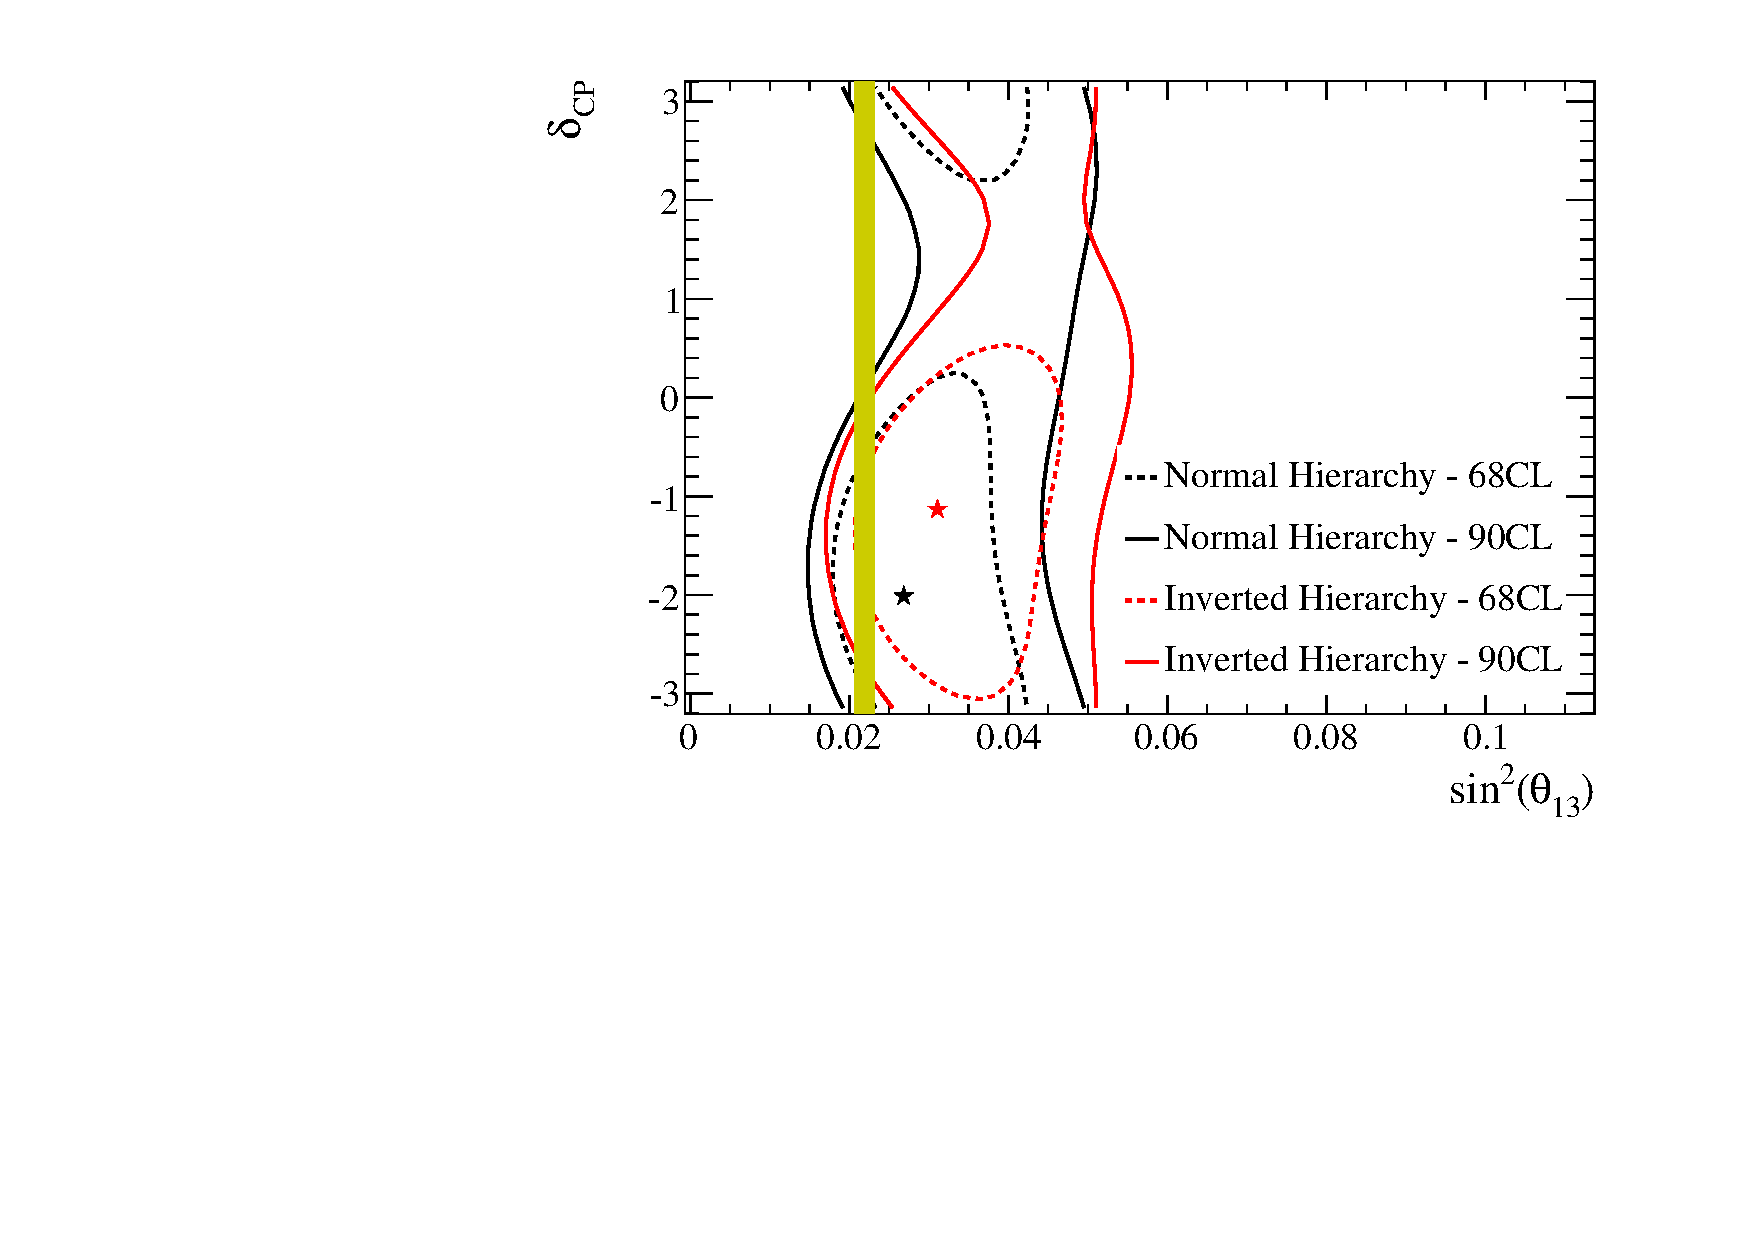
\includegraphics[width=0.9\textwidth]{joint_plots/data_contours/sinsqth13Vsdcp_t2konly_data_constdchisq.pdf}
\caption{$\sin^2 \theta_{13}$ Vs $\delta_{CP}$ with T2K data only}
\label{fig:ss13_dcp_t2k_only_data_fit}
\end{subfigure}
\begin{subfigure}[b]{0.49\textwidth}
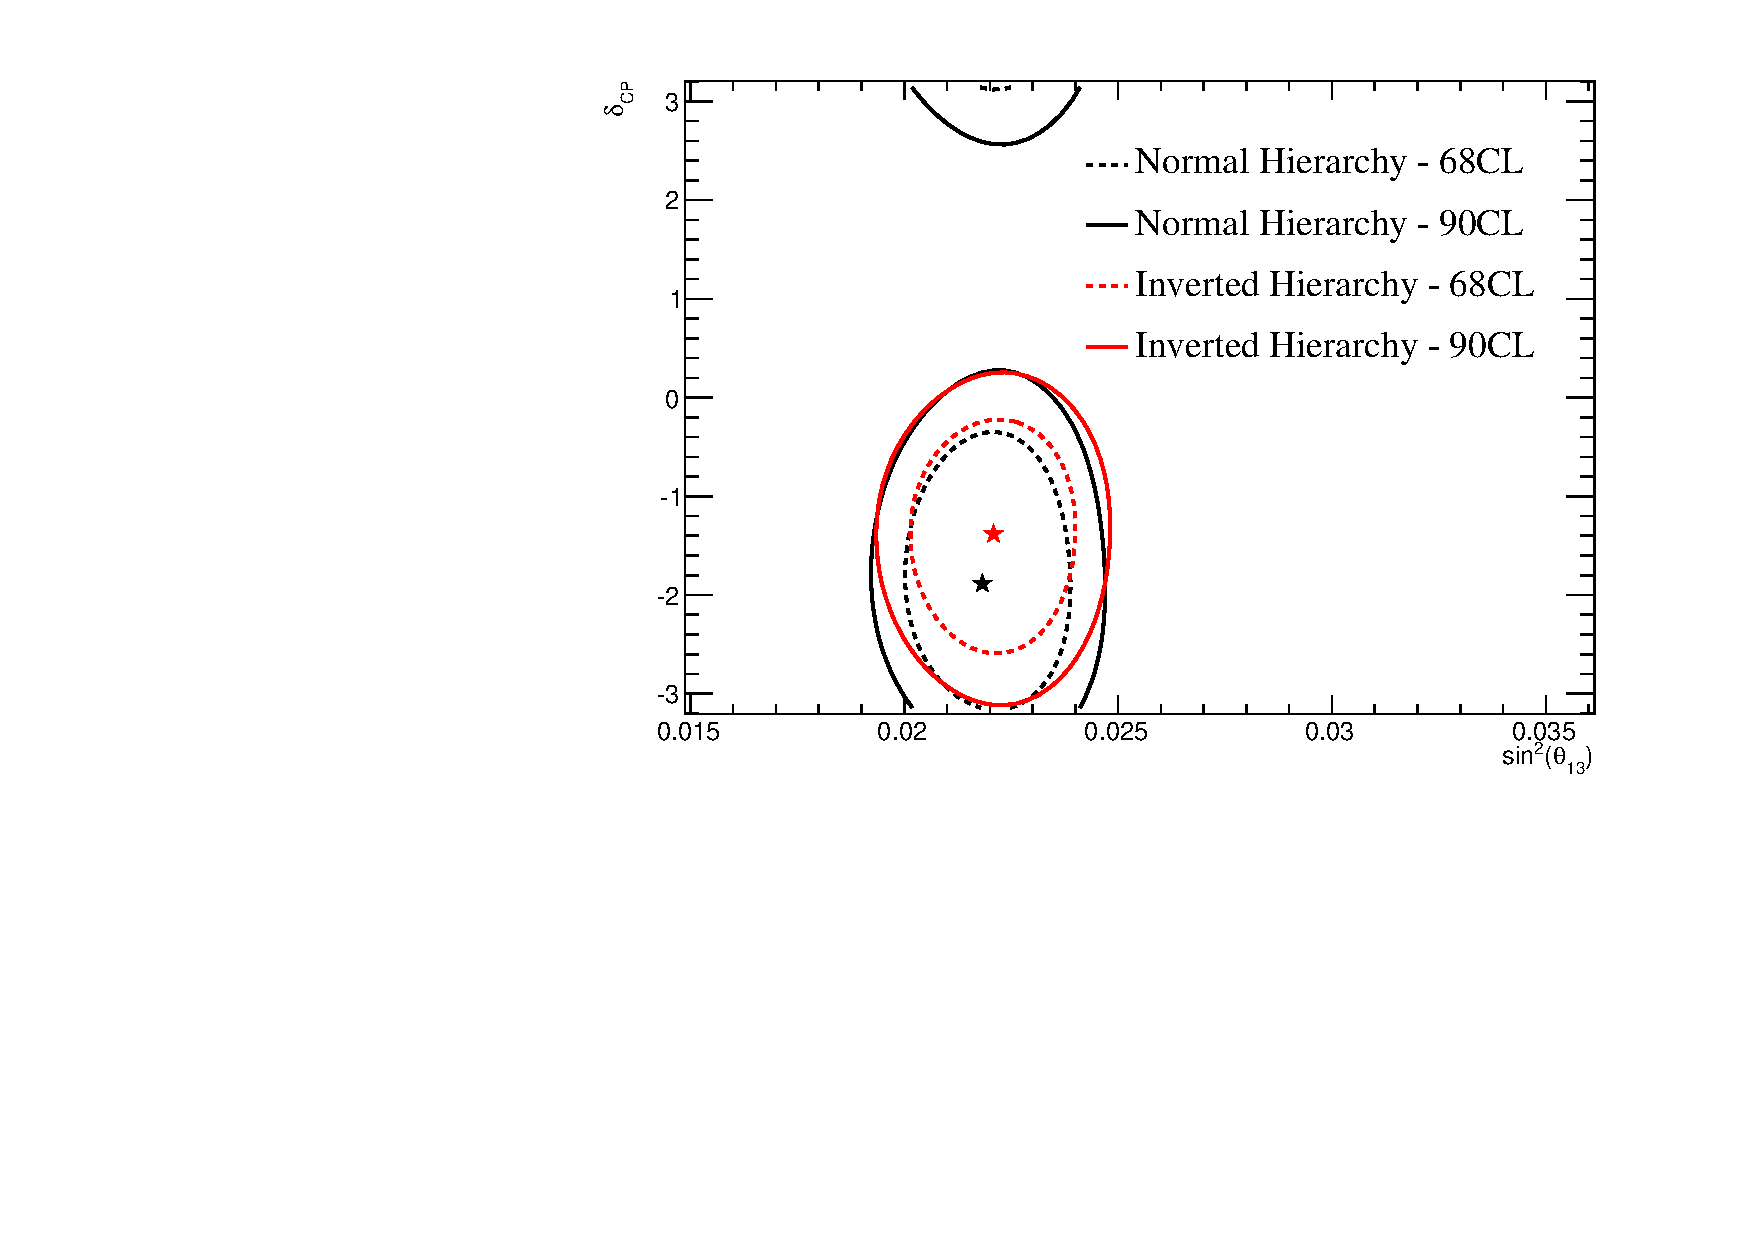
\includegraphics[width=0.9\textwidth]{joint_plots/data_contours/sinsqth13Vsdcp_react_data_constdchisq.pdf}
\caption{$\sin^2 \theta_{13}$ Vs $\delta_{CP}$ with reactor constraint}
\label{fig:ss13_dcp_with_reactor_data_fit}
\end{subfigure}
\begin{subfigure}[b]{0.49\textwidth}
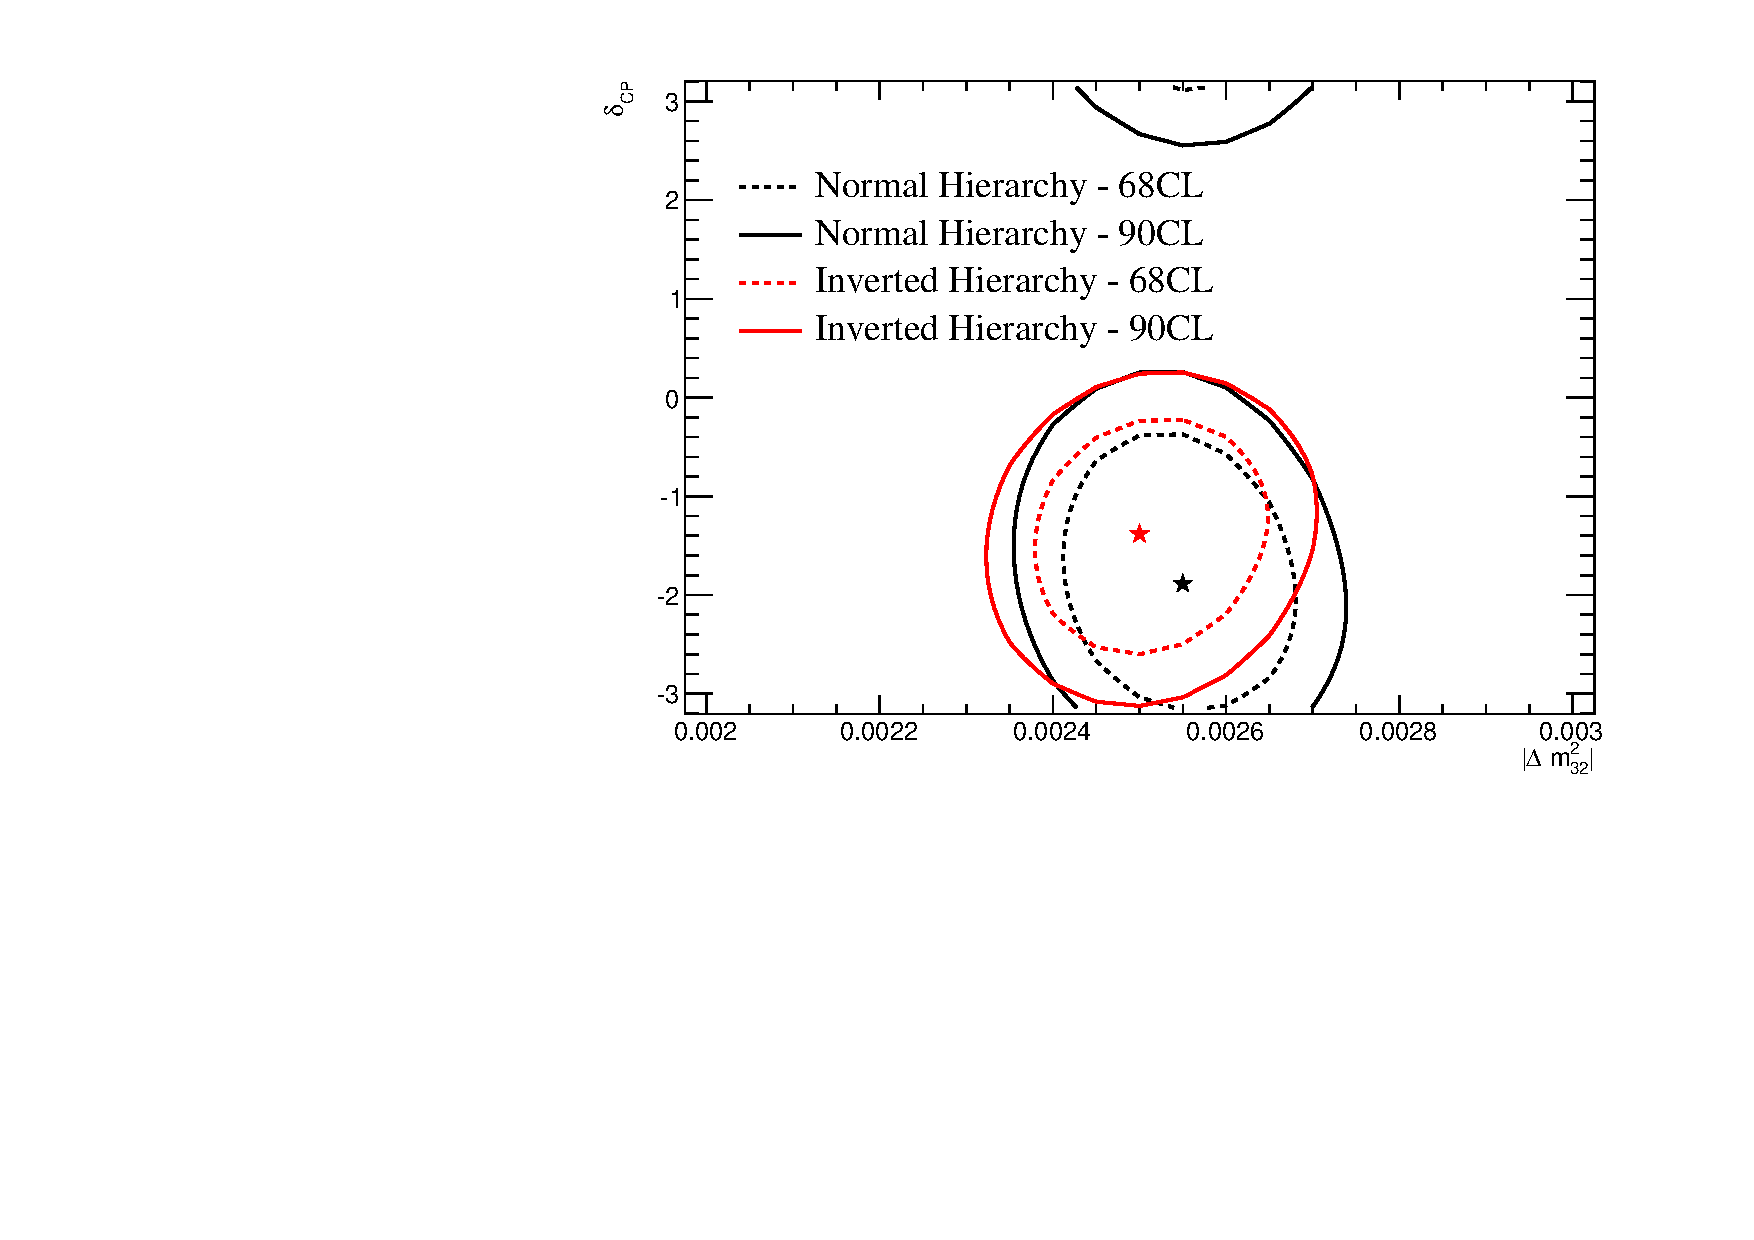
\includegraphics[width=0.9\textwidth]{joint_plots/data_contours/dmsqVsdcp_react_data_constdchisq.pdf}
\caption{$\Delta m^2_{32}$ ($\Delta m^2_{13}$) Vs $\delta_{CP}$ with reactor constraint}
\label{fig:dmsq_dcp_with_reactor_data_fit}
\end{subfigure}
\begin{subfigure}[b]{0.49\textwidth}
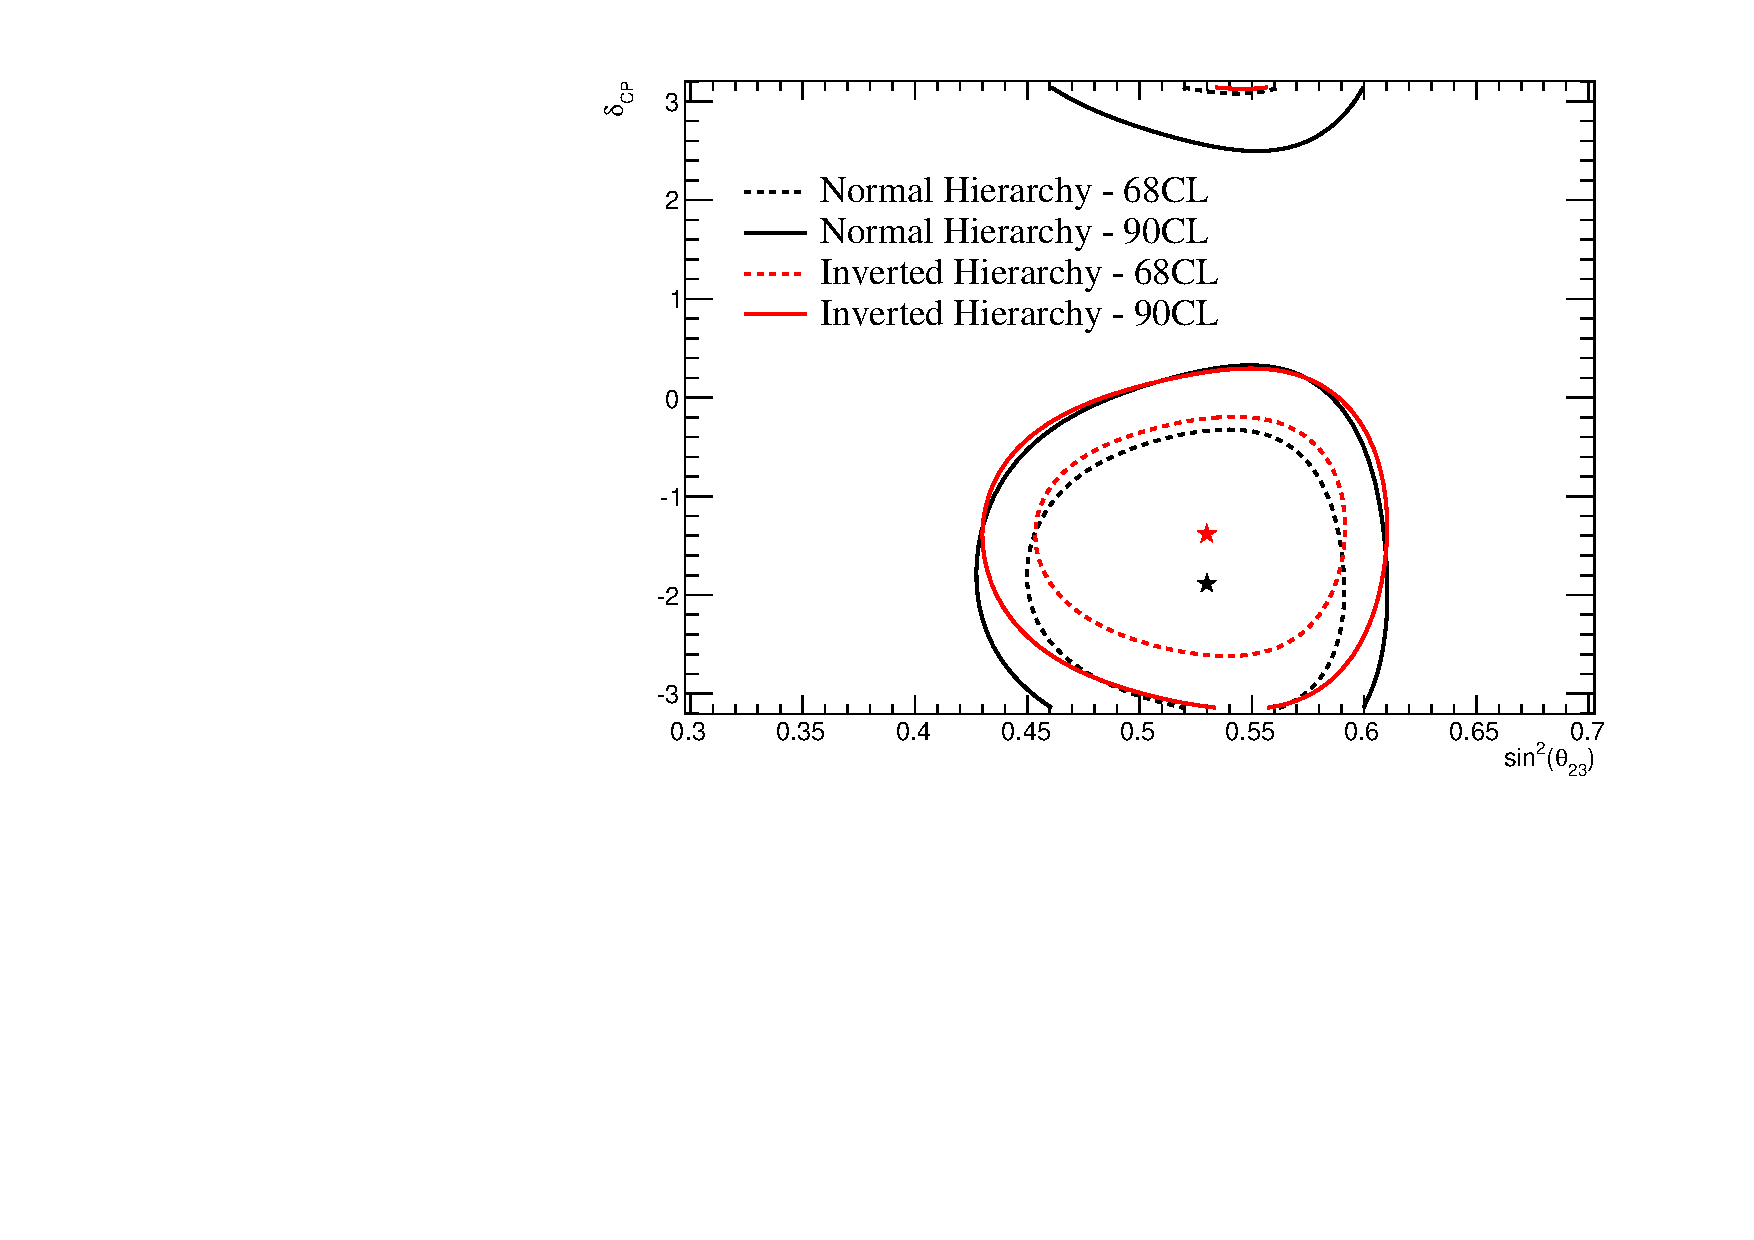
\includegraphics[width=0.9\textwidth]{joint_plots/data_contours/sinsqth23Vsdcp_react_data_constdchisq.pdf}
\caption{$\sin^2 \theta_{23}$ Vs $\delta_{CP}$ with reactor constraint}
\label{fig:ss23_dcp_with_reactor_data_fit}
\end{subfigure}
\begin{subfigure}[b]{0.49\textwidth}
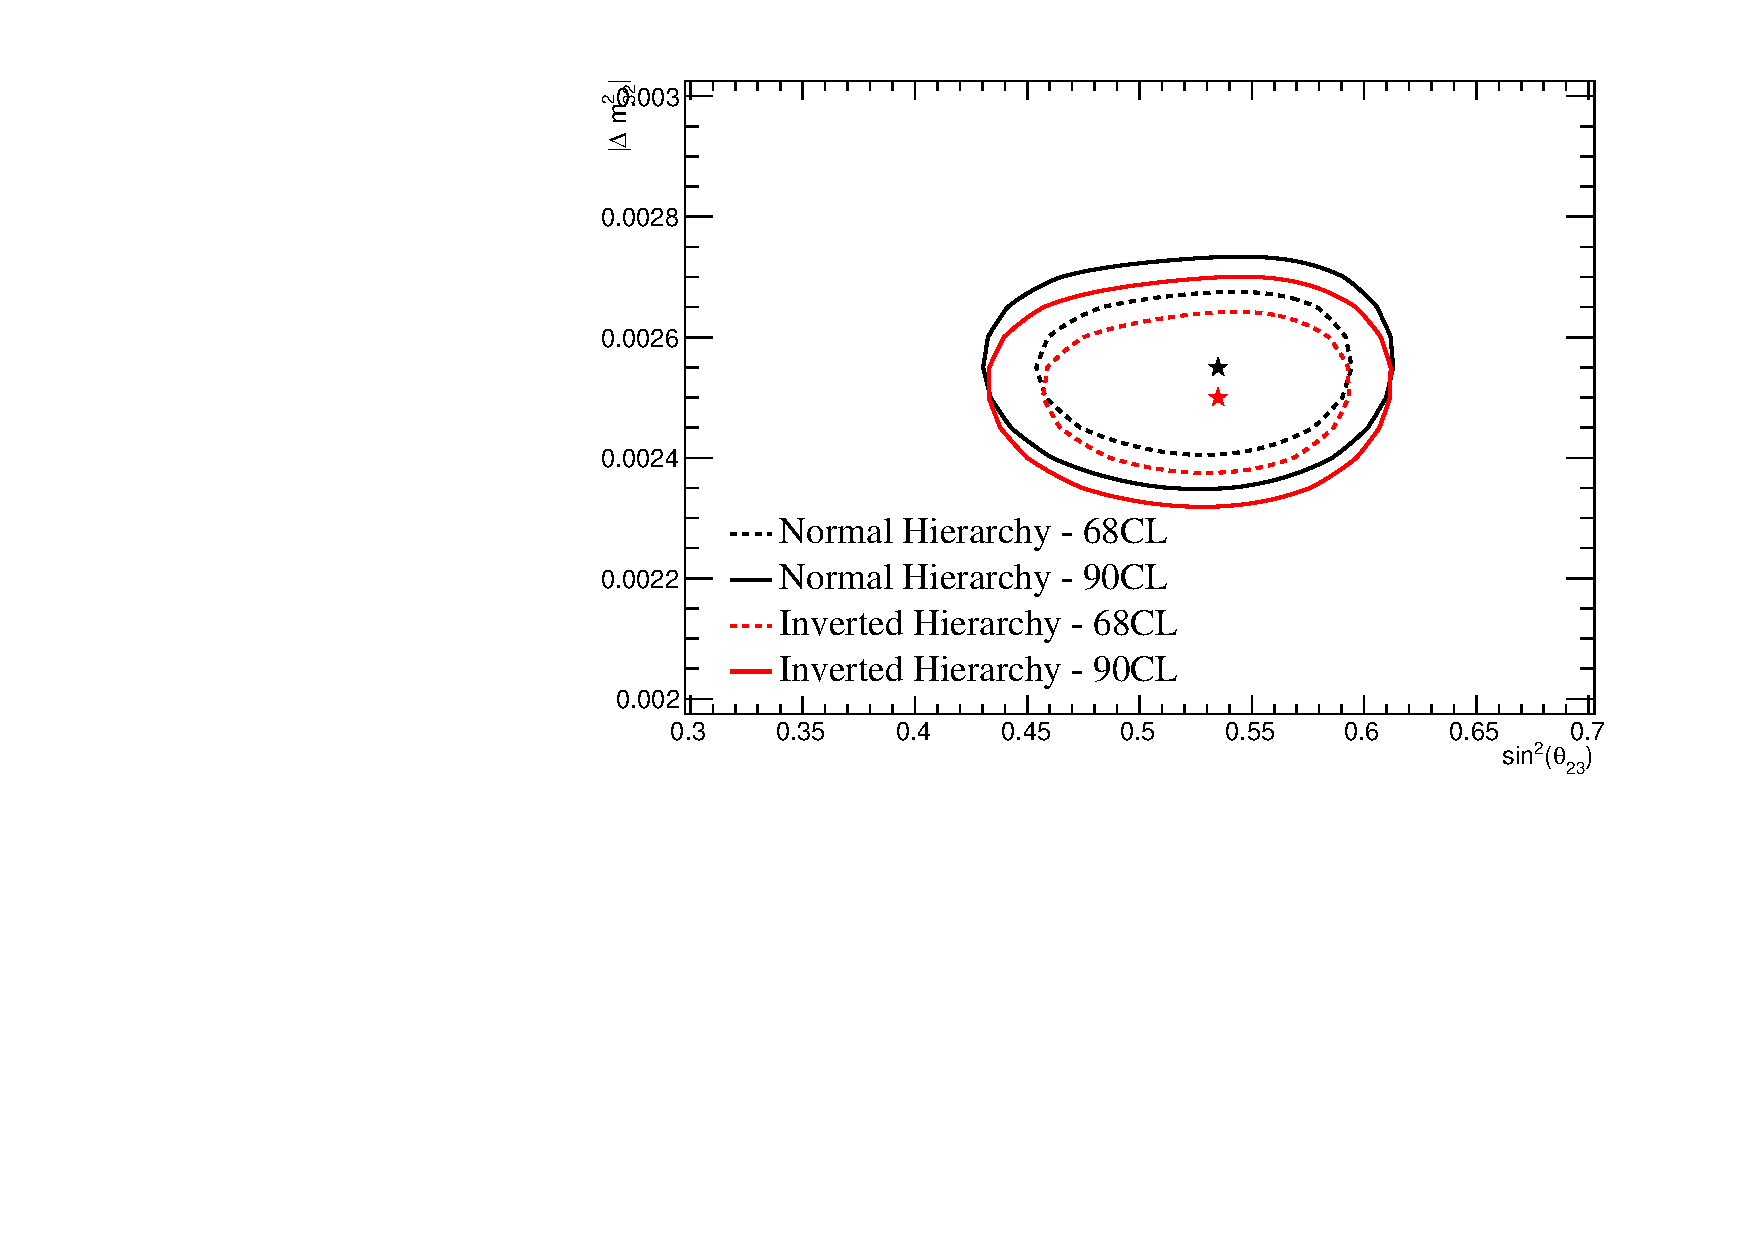
\includegraphics[width=0.9\textwidth]{joint_plots/data_contours/sinsqth23Vsdmsq_react_data_constdchisq.pdf}
\caption{$\sin^2 \theta_{23}$ Vs $\Delta m^2_{32}$ ($\Delta m^2_{13}$)
with reactor constraint}
\label{fig:ss23_dmsq_with_reactor_data_fit}
\end{subfigure}

%
\includegraphics[width=0.9\textwidth]{./images/missing_plot-eps-converted-to.pdf}
\caption{
%{\large{MEASURED 2D CONTOURS}}
Measured confidence intervals with the full run 1-6 data set.
Both normal (black) and inverted (red) hierarchies are shown. 
Both 68\% (dashed line) and 90\% CL (solid line) are shown.
Confidence intervals are produced using the \emph{constant} $\Delta \chi^2$ method. % (see app.~\ref{app:method_cl}).
Contours for normal (black) and inverted (red) hierarchy are computed independently
with respect to the global minimum of each hierarchy (star).
All the oscillation parameters which are not parameters of interest
are marginalised using the prior distributions shown in tab.~\ref{tab:osc_params_joint_priors}.
The measured contour of $\sin^2 \theta_{13}$ Vs $\delta_{CP}$ without reactor constraint, in Fig~\ref{fig:ss13_dcp_t2k_only_data_fit} is compared with the measurement by reactor experiments, 
$\sin^2 \theta_{13} = 0.0219 \pm 0.0012 $
\cite{pdg_2014},
shown by the yellow bar.
}
\label{fig:joint_sensi_t2krun14bf_2d}
\end{figure*}


\begin{figure*}[htb]
\center
\begin{subfigure}[b]{0.49\textwidth}
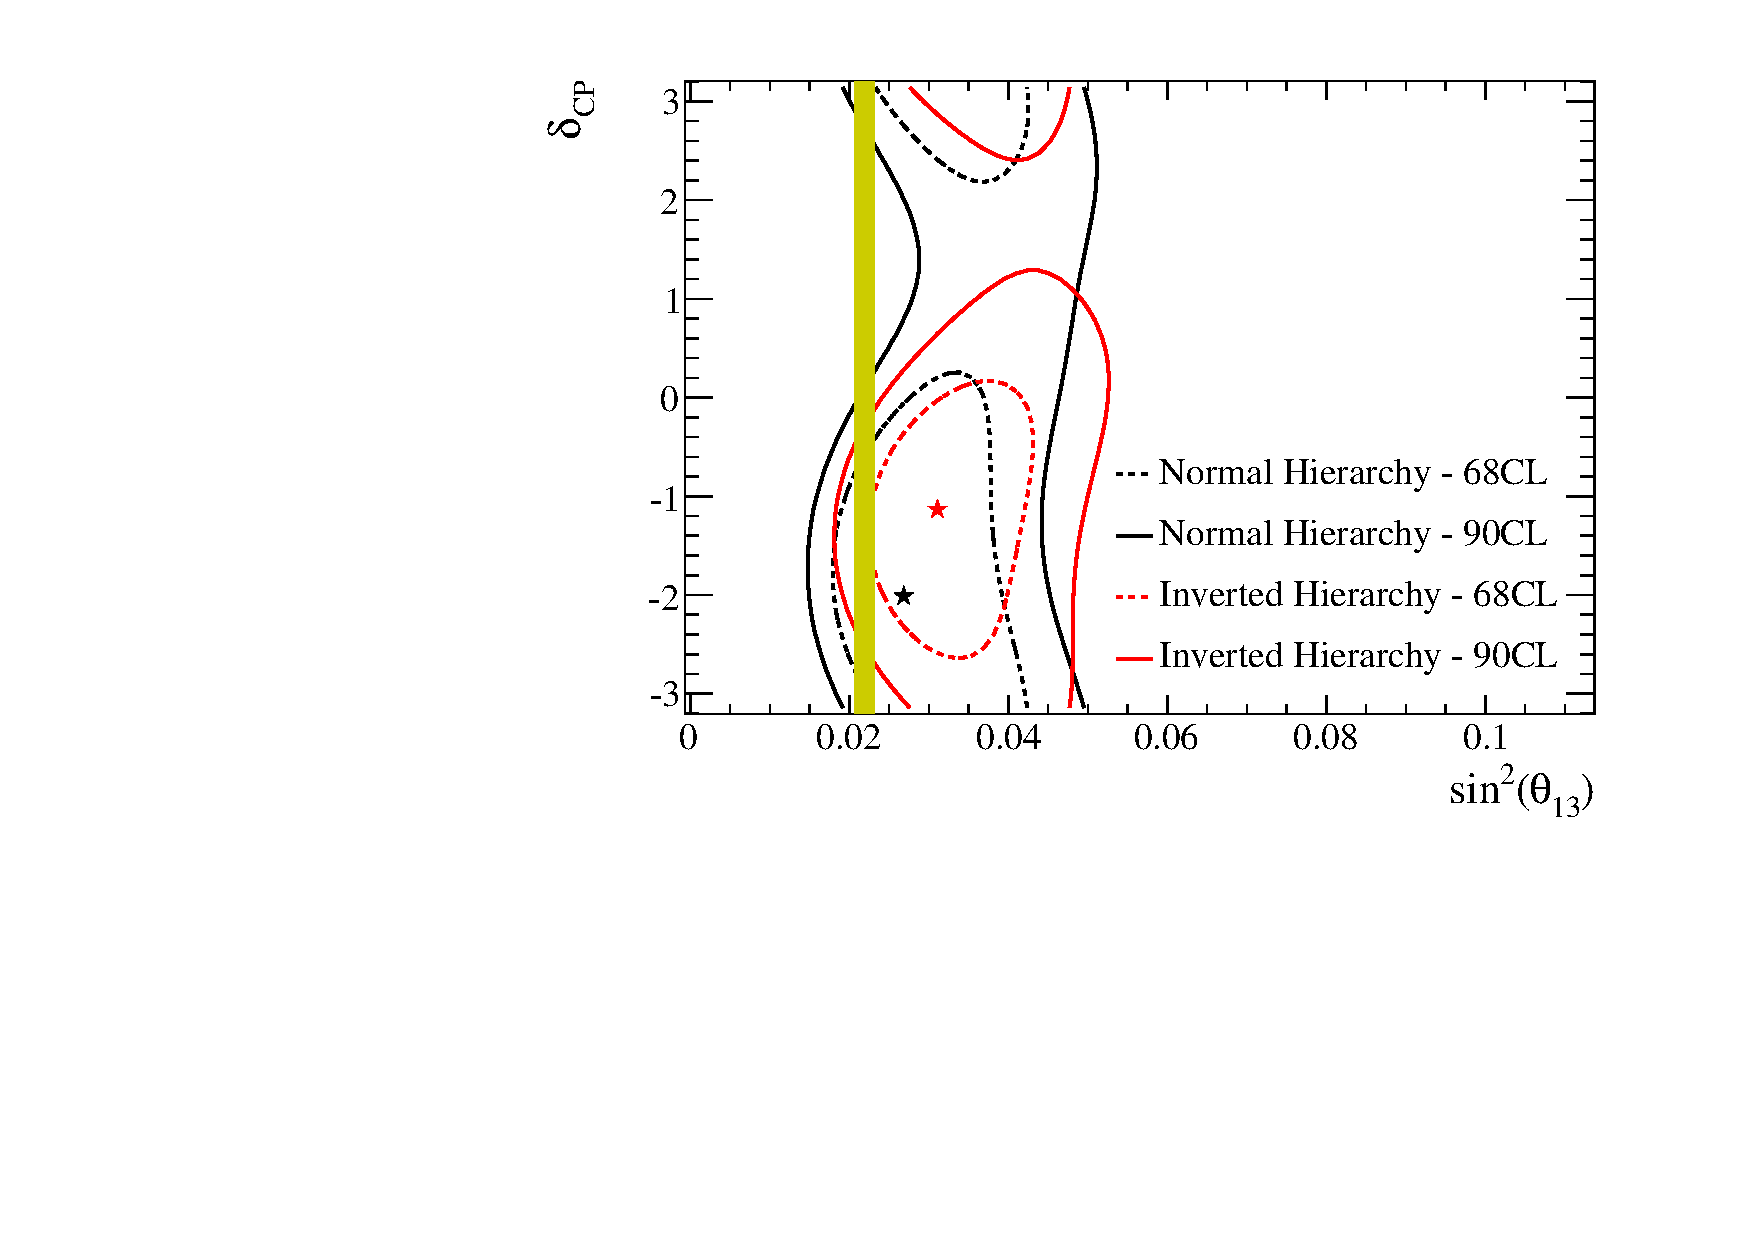
\includegraphics[width=0.9\textwidth]{joint_plots/data_contours/sinsqth13Vsdcp_t2konly_data_constdchisq_glob.pdf}
\caption{$\sin^2 \theta_{13}$ Vs $\delta_{CP}$ with T2K data only}
\label{fig:ss13_dcp_t2k_only_data_fit_global}
\end{subfigure}
\begin{subfigure}[b]{0.49\textwidth}
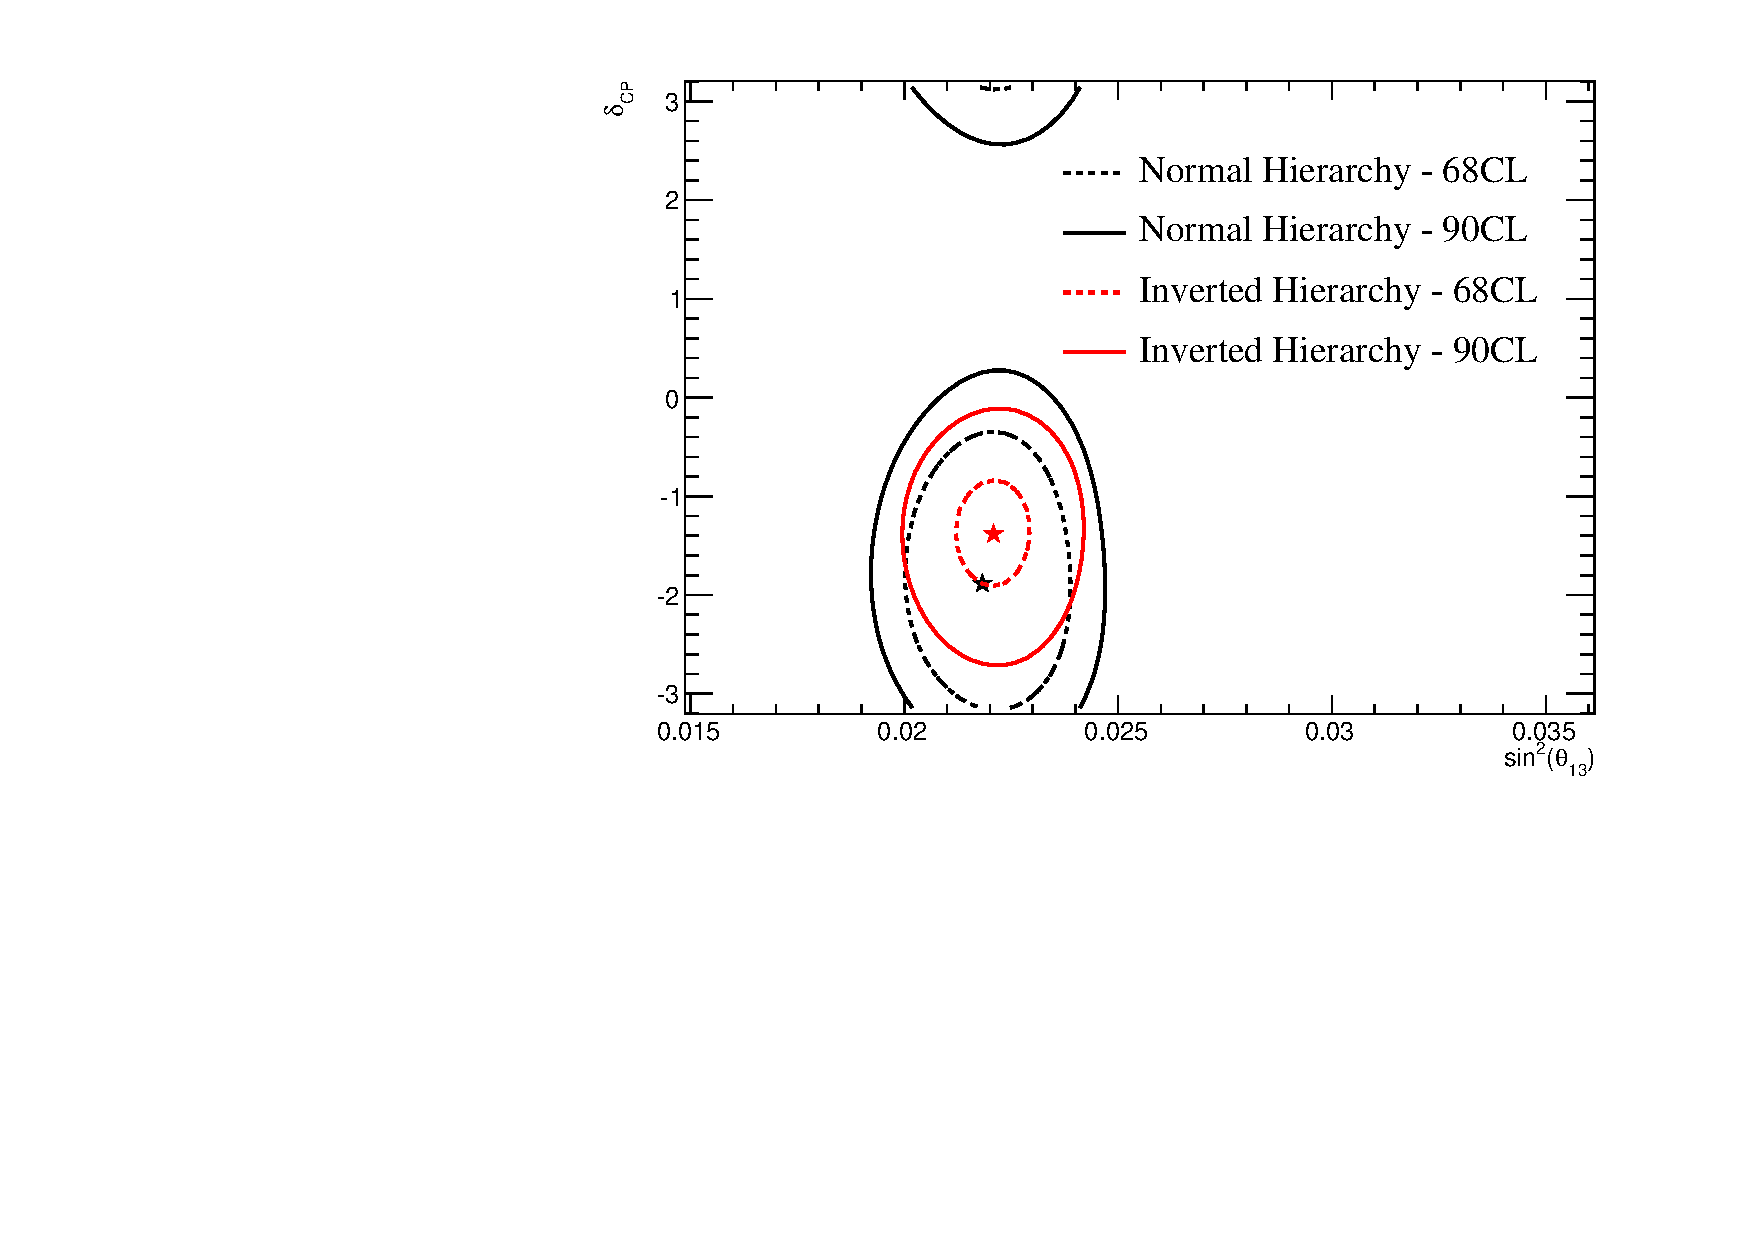
\includegraphics[width=0.9\textwidth]{joint_plots/data_contours/sinsqth13Vsdcp_react_data_constdchisq_glob.pdf}
\caption{$\sin^2 \theta_{13}$ Vs $\delta_{CP}$ with reactor constraint}
\end{subfigure}
\begin{subfigure}[b]{0.49\textwidth}
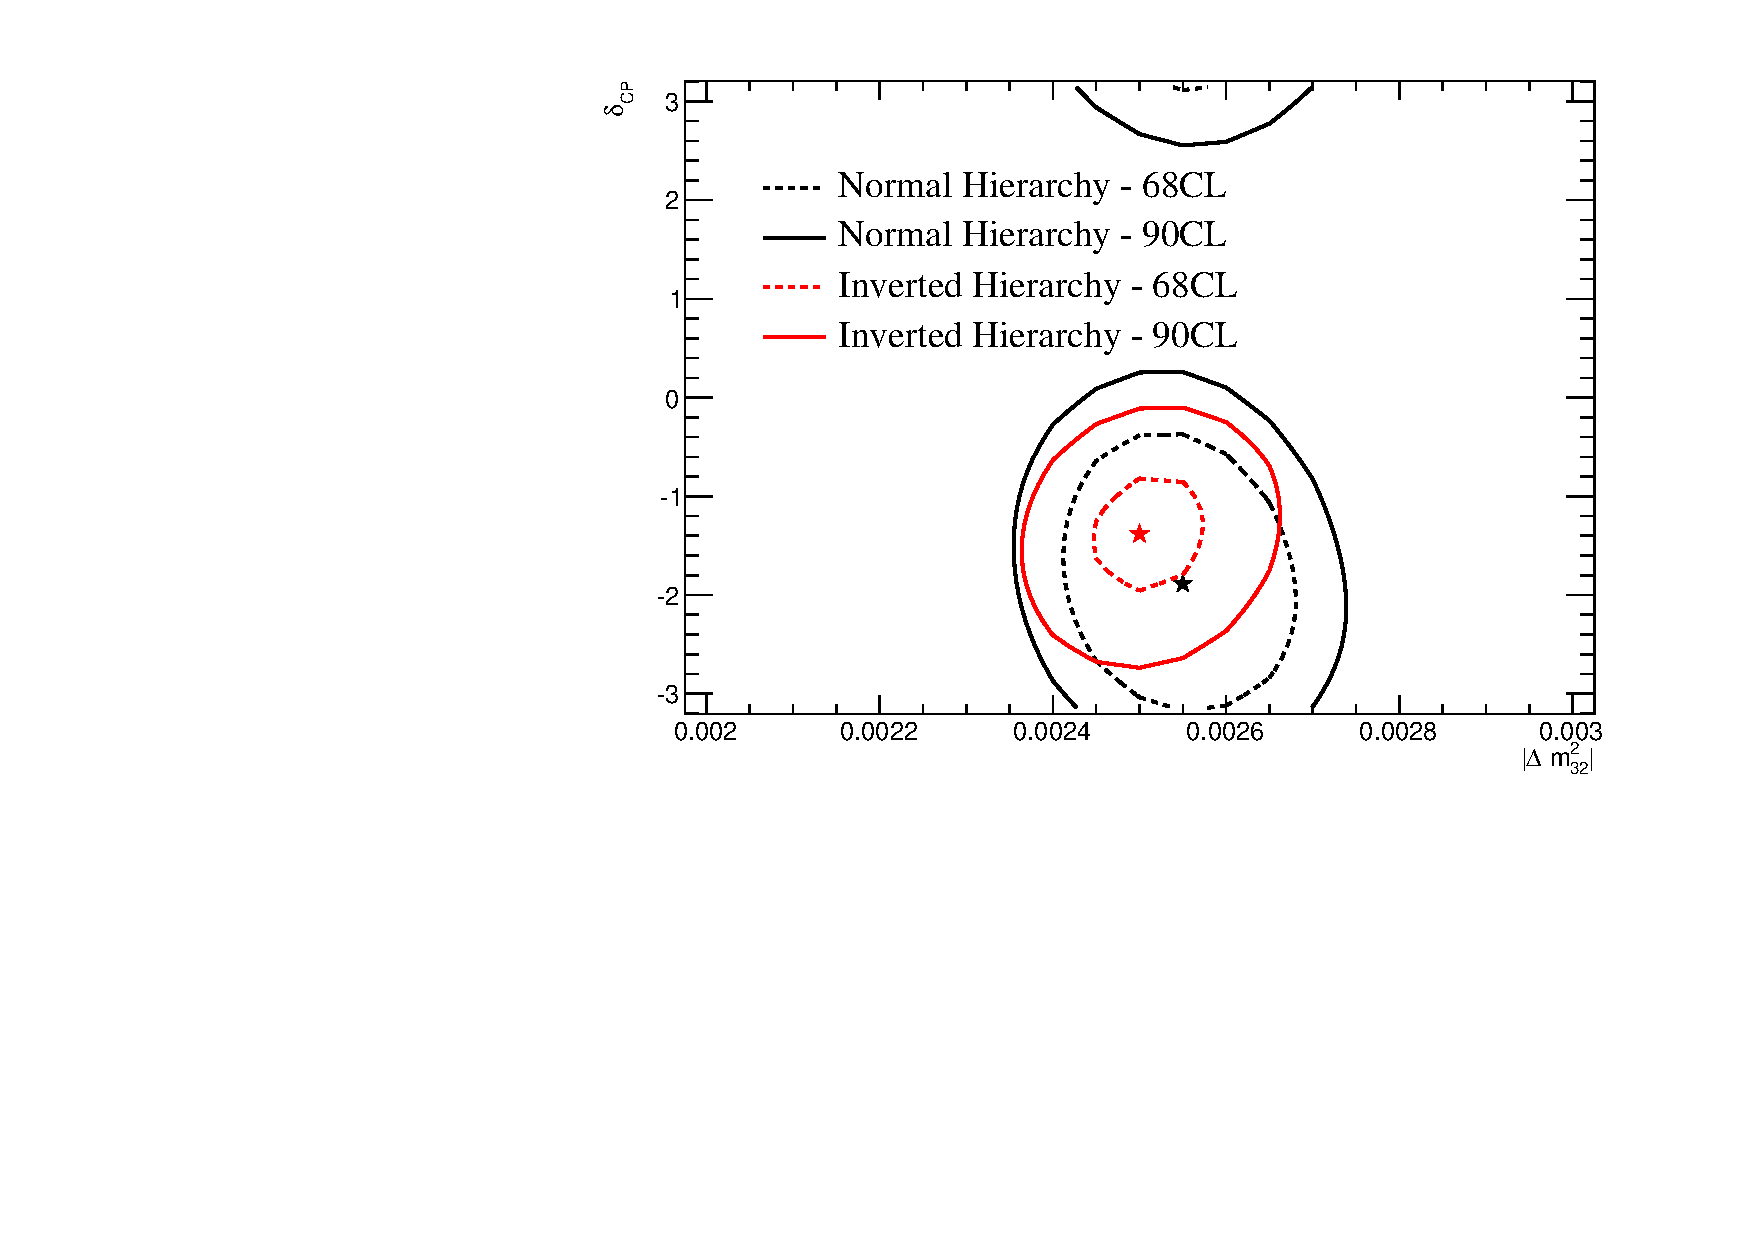
\includegraphics[width=0.9\textwidth]{joint_plots/data_contours/dmsqVsdcp_react_data_constdchisq_glob.pdf}
\caption{$\Delta m^2_{32}$ ($\Delta m^2_{13}$) Vs $\delta_{CP}$ with reactor constraint}
\end{subfigure}
\begin{subfigure}[b]{0.49\textwidth}
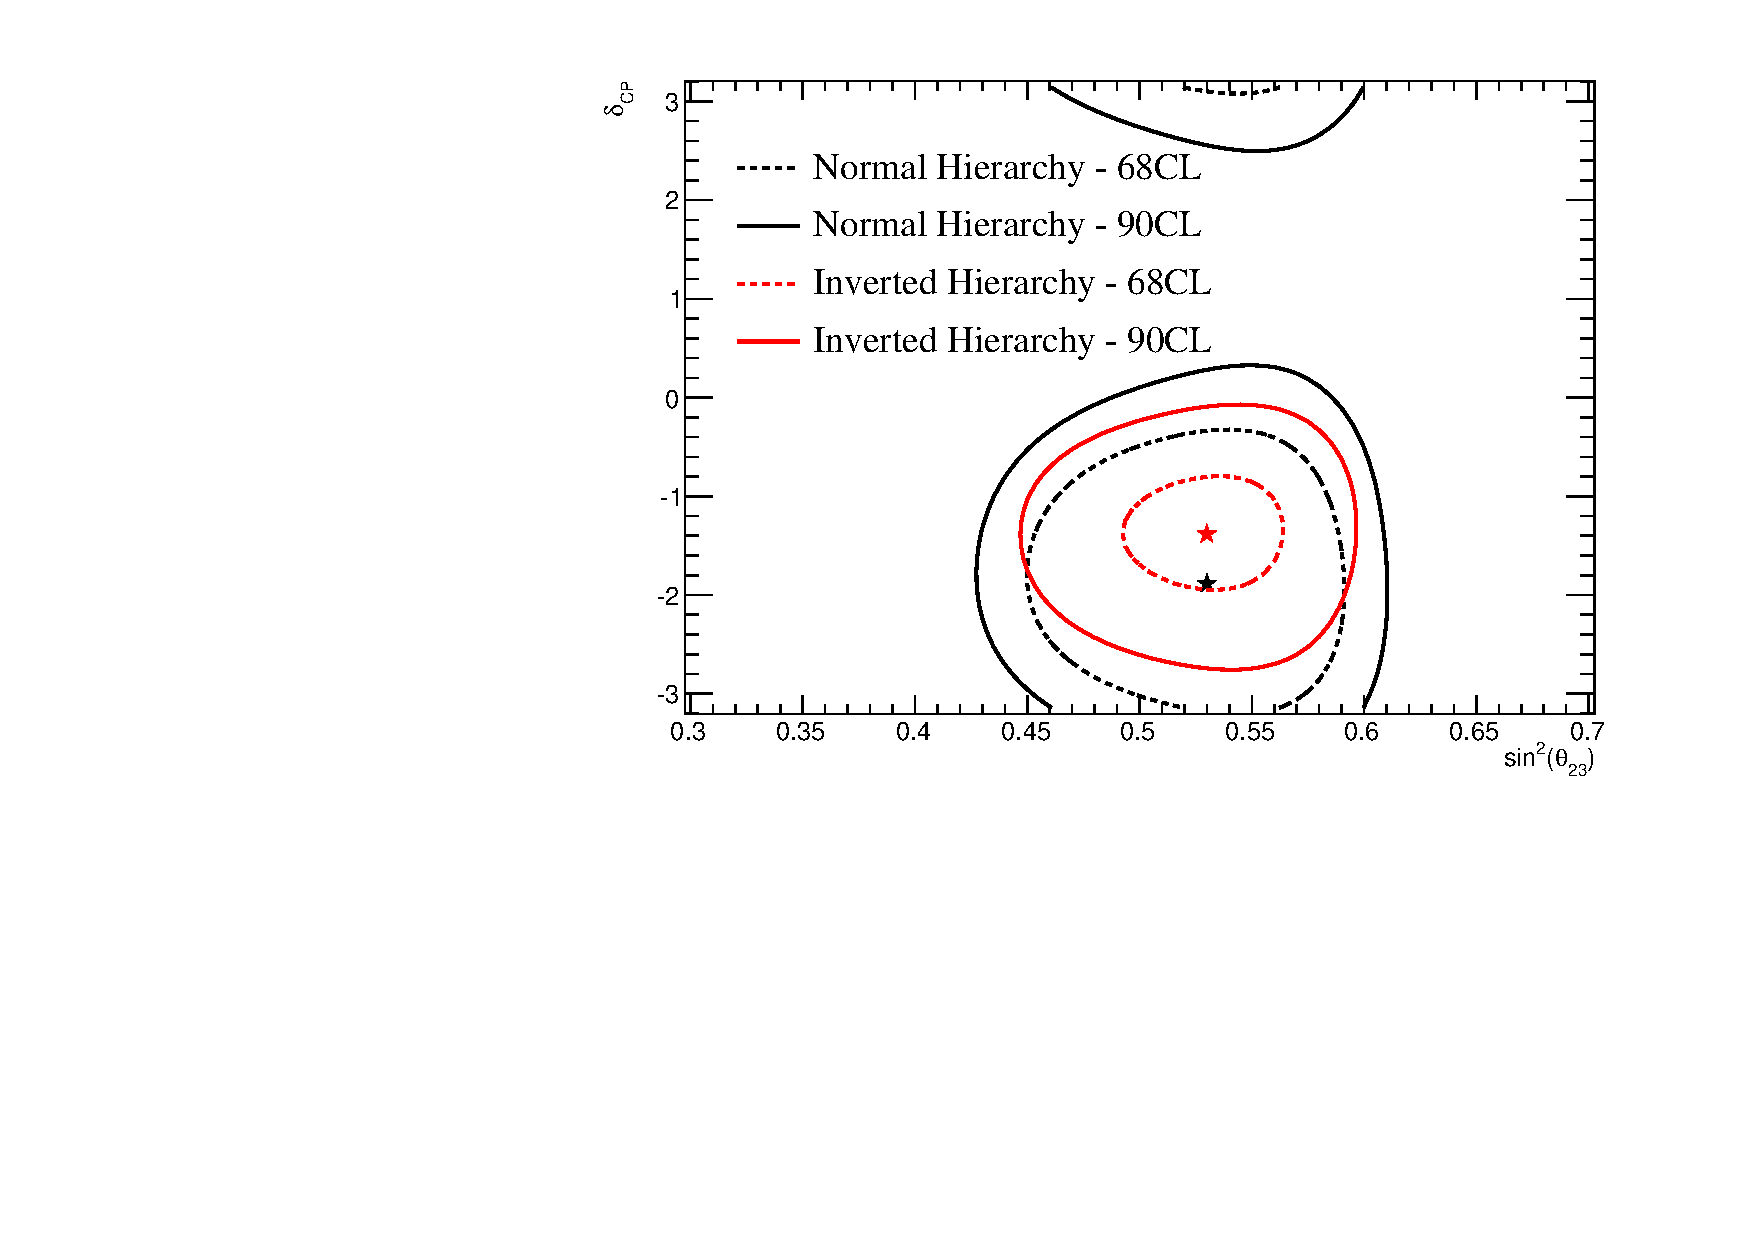
\includegraphics[width=0.9\textwidth]{joint_plots/data_contours/sinsqth23Vsdcp_react_data_constdchisq_glob.pdf}
\caption{$\sin^2 \theta_{23}$ Vs $\delta_{CP}$ with reactor constraint}
\end{subfigure}
\begin{subfigure}[b]{0.49\textwidth}
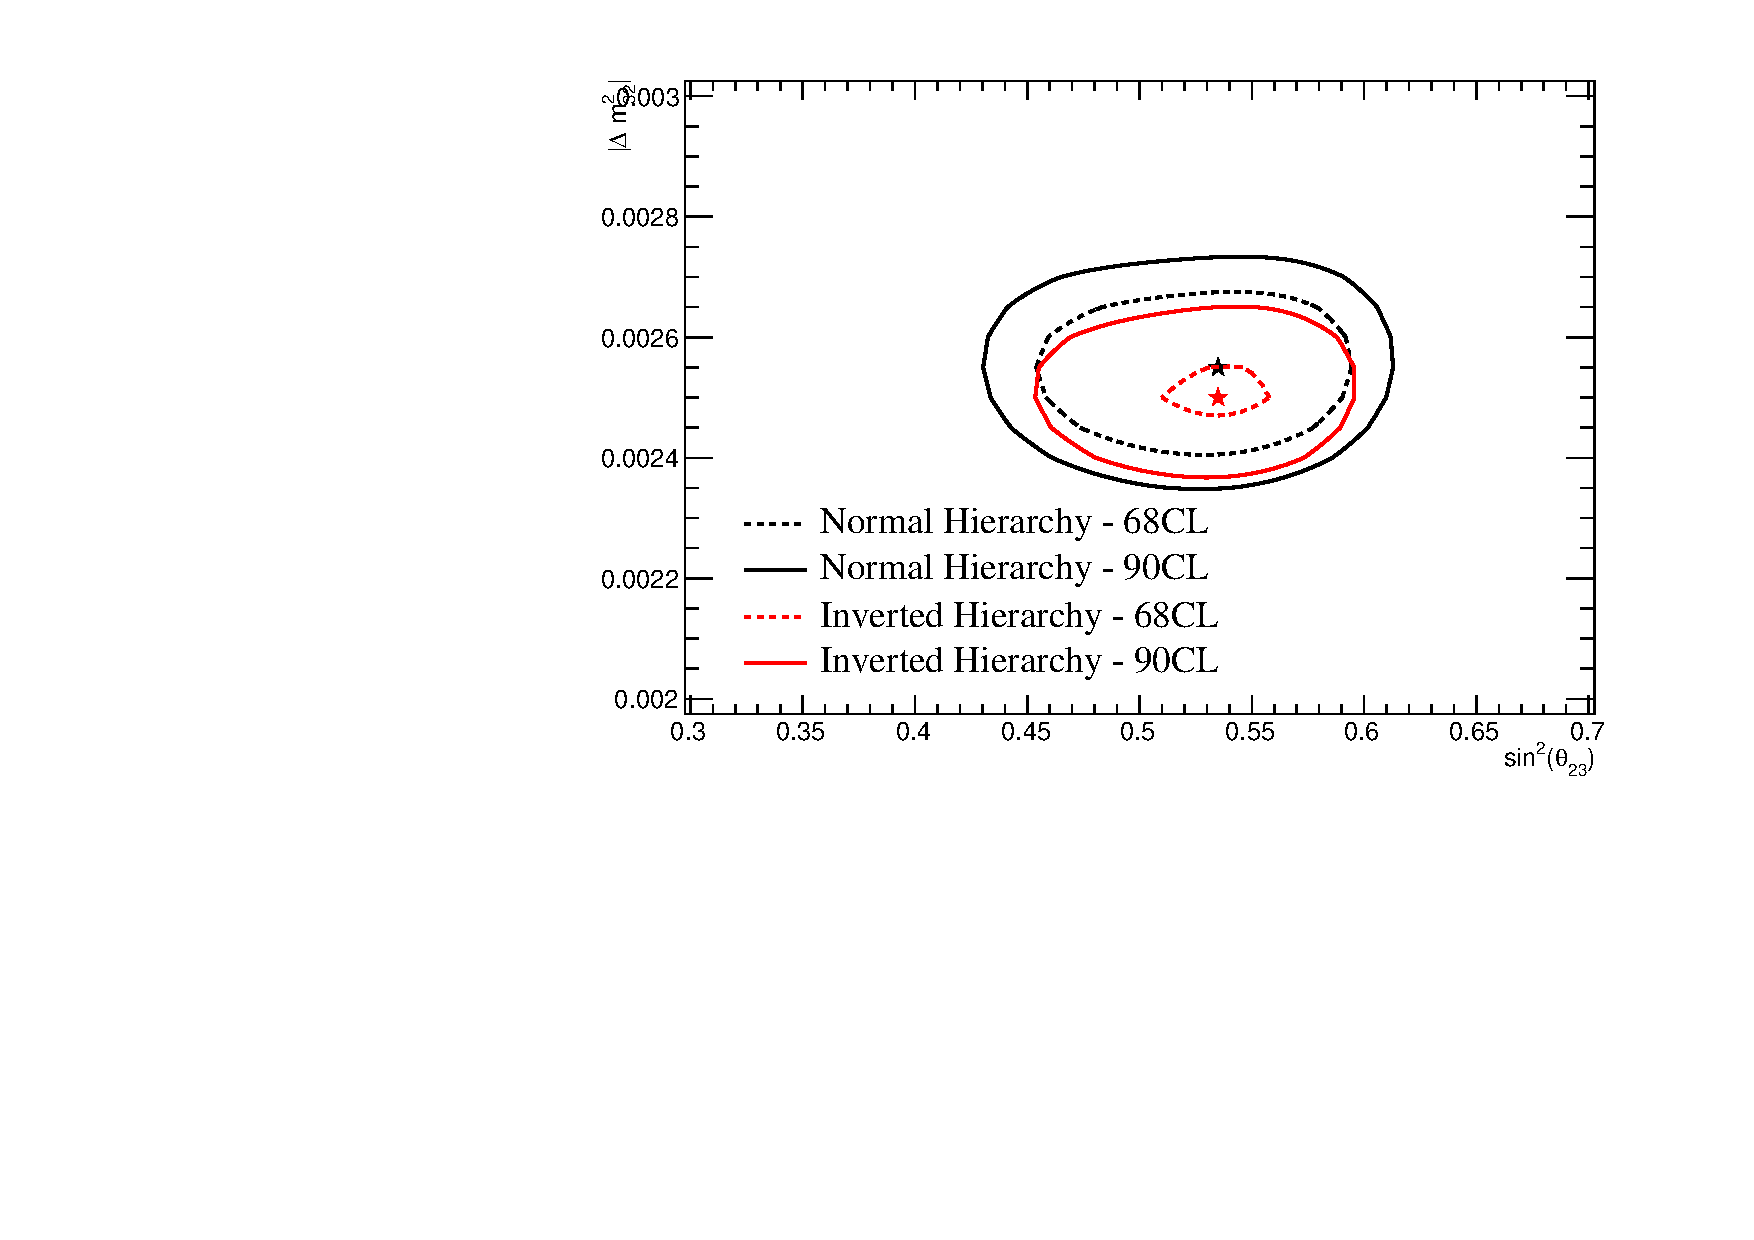
\includegraphics[width=0.9\textwidth]{joint_plots/data_contours/sinsqth23Vsdmsq_react_data_constdchisq_glob.pdf}
\caption{$\sin^2 \theta_{23}$ Vs $\Delta m^2_{32}$ ($\Delta m^2_{13}$)
with reactor constraint}
\end{subfigure}
%
\includegraphics[width=0.9\textwidth]{./images/missing_plot-eps-converted-to.pdf}
%
\includegraphics[width=0.9\textwidth]{./images/missing_plot-eps-converted-to.pdf}
%
\includegraphics[width=0.9\textwidth]{./images/missing_plot-eps-converted-to.pdf}
%
\includegraphics[width=0.9\textwidth]{./images/missing_plot-eps-converted-to.pdf}
%
\includegraphics[width=0.9\textwidth]{./images/missing_plot-eps-converted-to.pdf}
\caption{
%{\large{MEASURED 2D CONTOURS}}
Measured confidence intervals 
with the full run 1-6 data set.
Both normal (black) and inverted (red) hierarchies are shown. 
Contours for normal (black) and inverted (red) hierarchy are computed 
with respect to the minimum of the best-fit hierarchy (star), which
corresponds to normal hierarchy.
Both 68\% (dashed line) and 90\% CL (solid line) are shown.
Confidence intervals are produced using the \emph{constant} $\Delta \chi^2$ method. % (see app.~\ref{app:method_cl}).
All the oscillation parameters which are not parameters of interest
are marginalised using the prior distributions shown in tab.~\ref{tab:osc_params_joint_priors}.
The measured contour of $\sin^2 \theta_{13}$ Vs $\delta_{CP}$ without reactor constraint
is compared with the measurement by reactor experiments, 
$\sin^2 \theta_{13} = 0.0219 \pm 0.0012 $
\cite{pdg_2014},
shown by the yellow bar.
}
\label{fig:joint_sensi_t2krun14bf_2d_glob}
\end{figure*}


\begin{figure*}[htb]
\center
\begin{subfigure}[b]{0.49\textwidth}
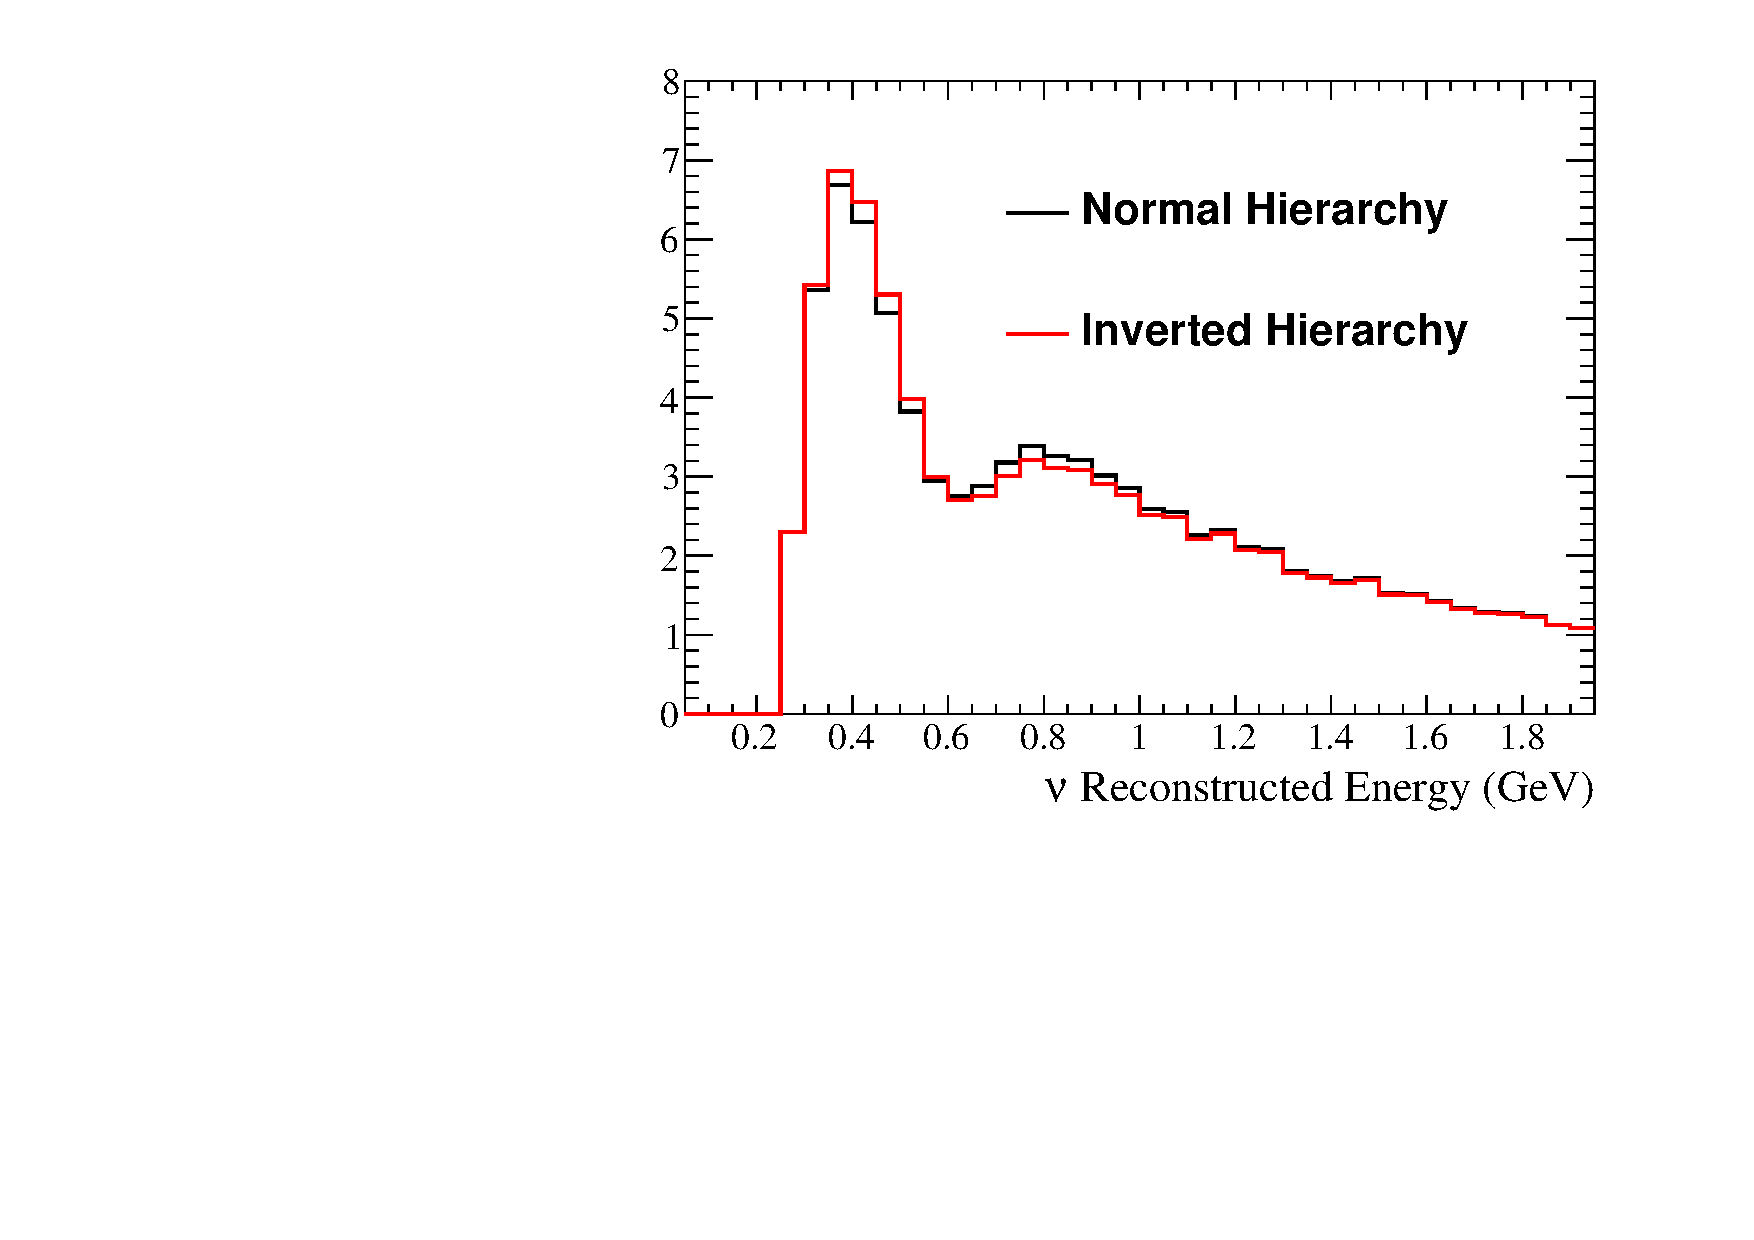
\includegraphics[width=0.9\textwidth]{joint_plots/spectrum_predictions/ereco_nh_Vs_ih_Asimov_A_1Rmu.pdf}
\caption{Muon-like, neutrino mode}
\end{subfigure}
\begin{subfigure}[b]{0.49\textwidth}
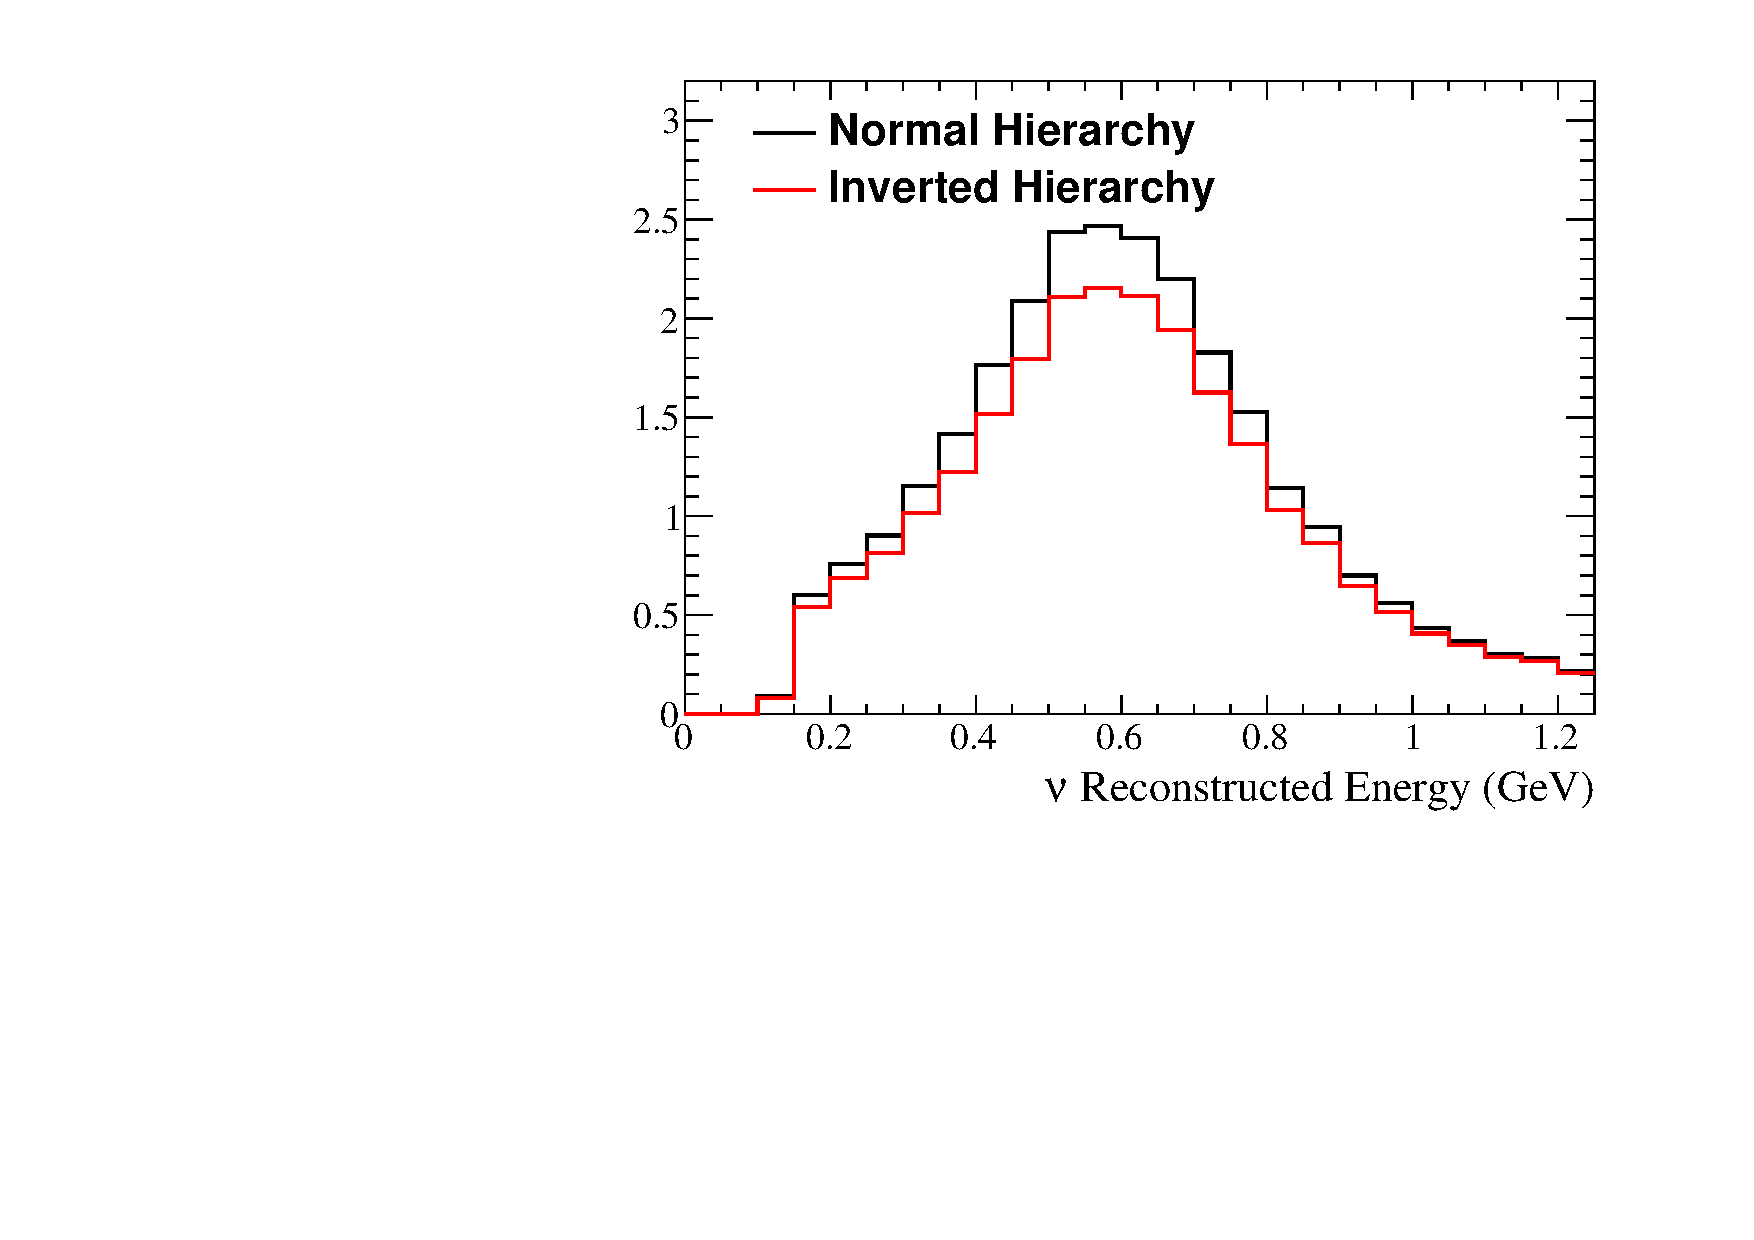
\includegraphics[width=0.9\textwidth]{joint_plots/spectrum_predictions/ereco_nh_Vs_ih_Asimov_A_1Re.pdf}
\caption{Electron-like, neutrino mode}
\end{subfigure}
\begin{subfigure}[b]{0.49\textwidth}
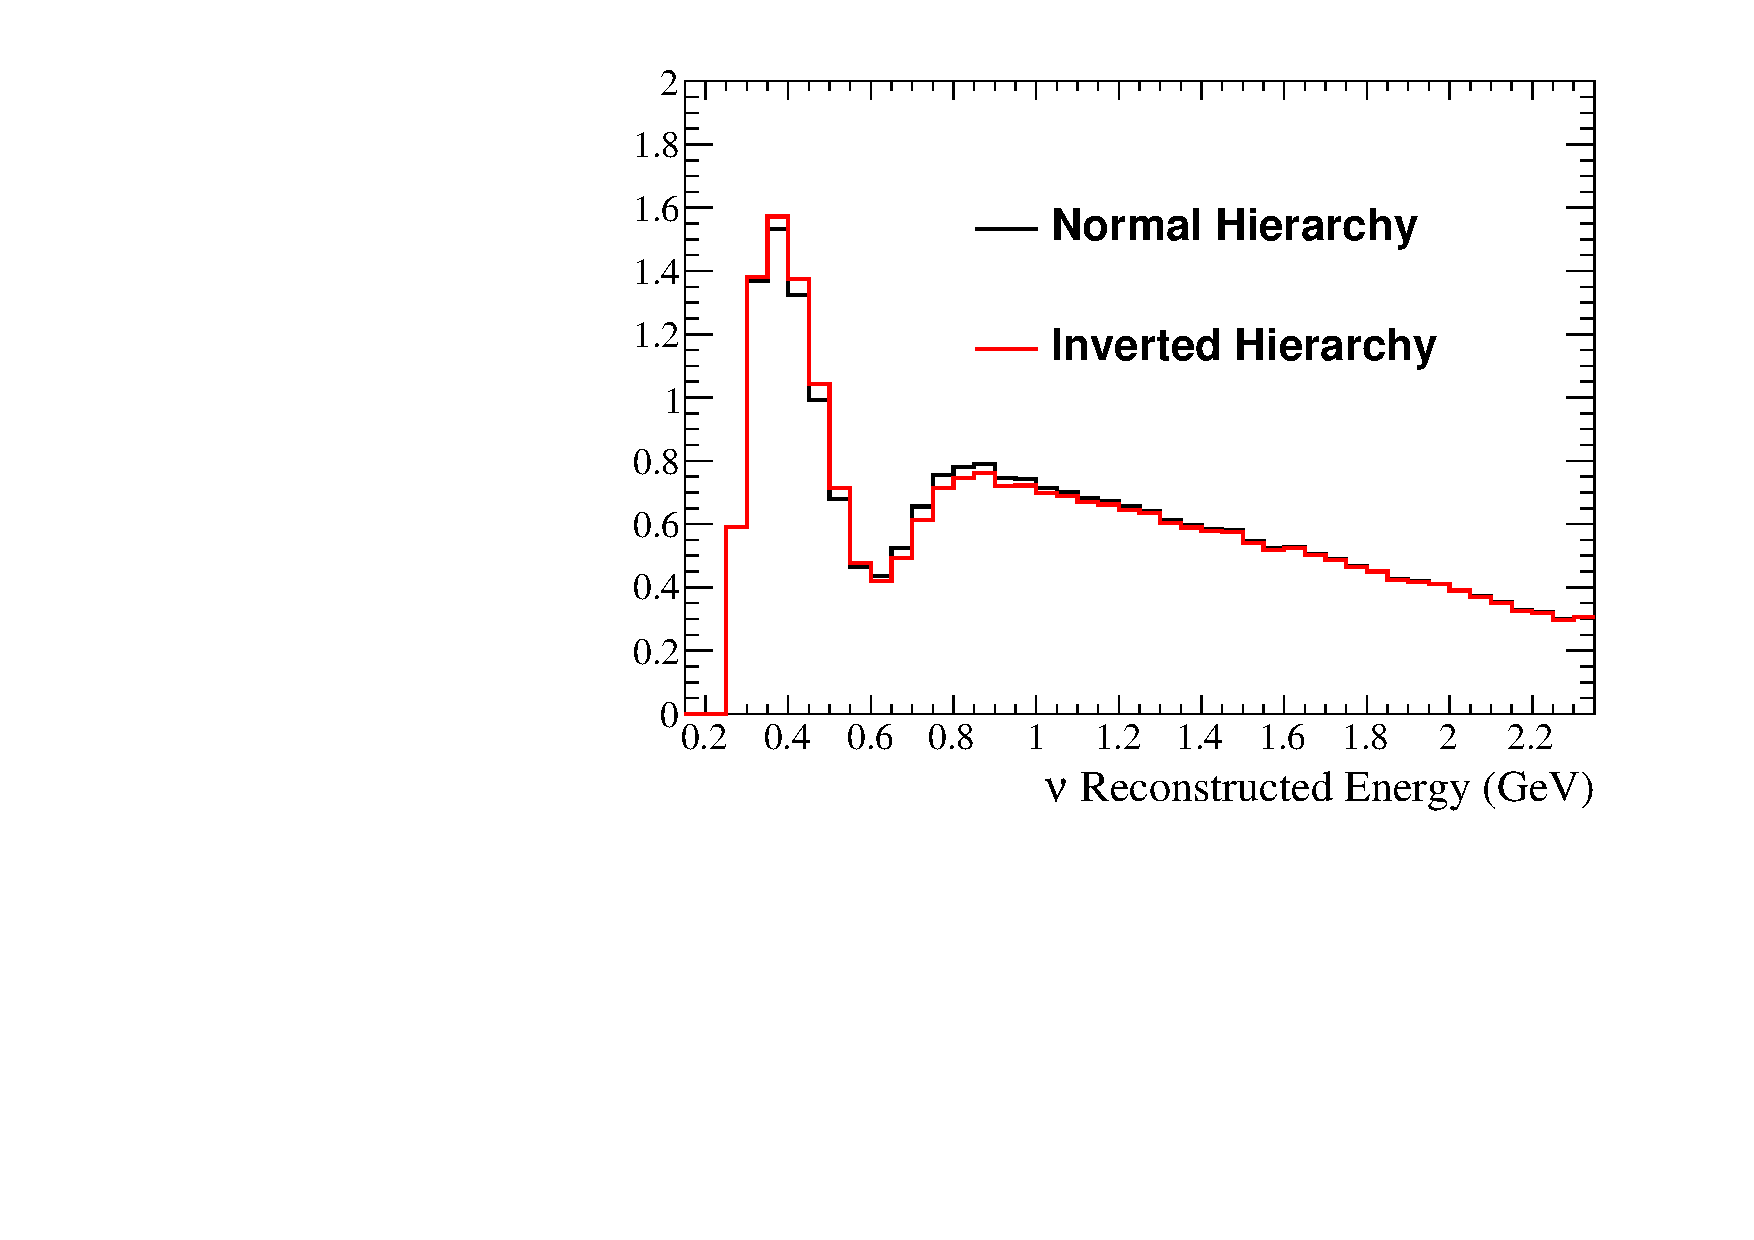
\includegraphics[width=0.9\textwidth]{joint_plots/spectrum_predictions/ereco_nh_Vs_ih_Asimov_A_RHC1Rmu.pdf}
\caption{Muon-like, antineutrino mode}
\end{subfigure}
\begin{subfigure}[b]{0.49\textwidth}
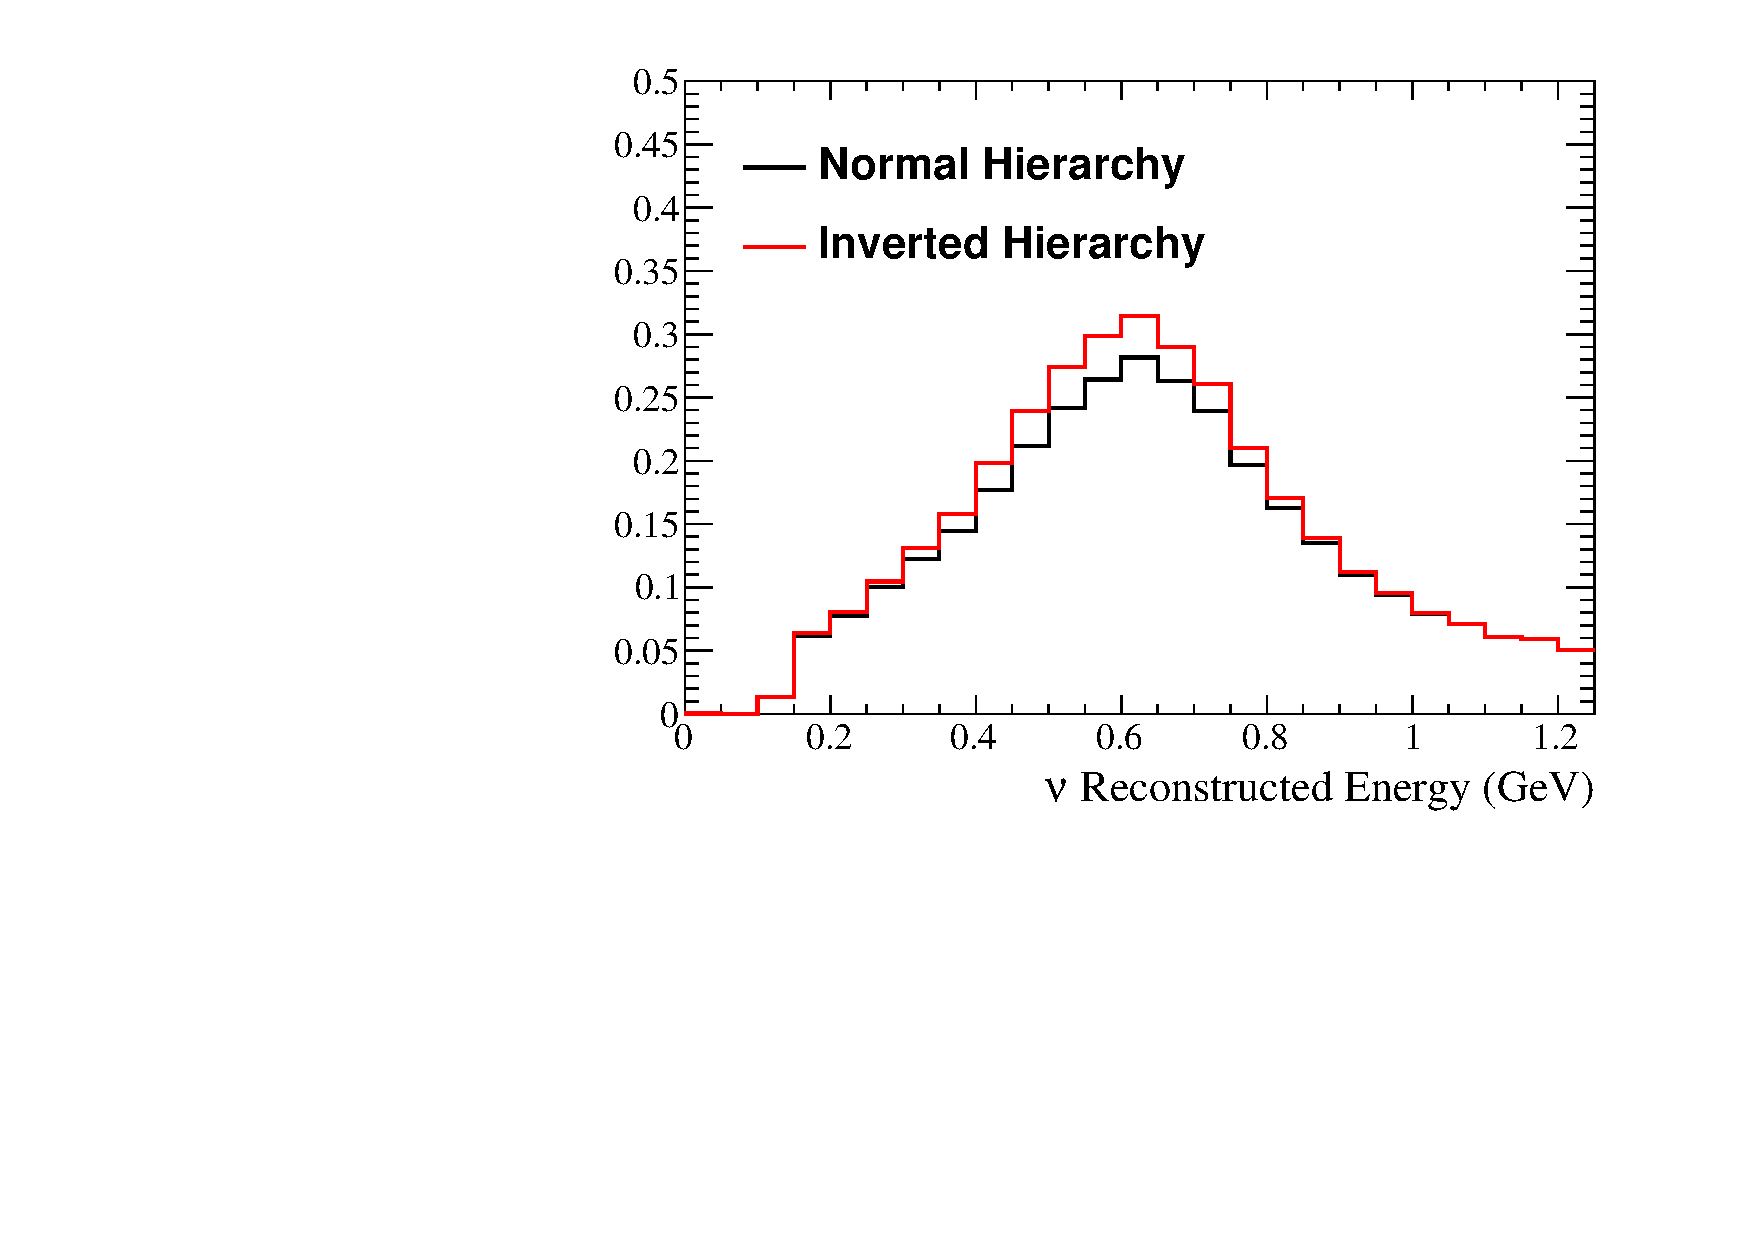
\includegraphics[width=0.9\textwidth]{joint_plots/spectrum_predictions/ereco_nh_Vs_ih_Asimov_A_RHC1Re.pdf}
\caption{Electron-like, antineutrino mode}
\end{subfigure}
%\includegraphics[width=0.9\textwidth]{joint_plots/data/1rmu_ereco_tot_osc_notosc_bf.pdf}
%\includegraphics[width=0.9\textwidth]{joint_plots/data/rhc1rmu_ereco_tot_osc_notosc_bf.pdf}
%\includegraphics[width=0.9\textwidth]{joint_plots/data/1re_ereco_tot_osc_notosc_bf.pdf}
%\includegraphics[width=0.9\textwidth]{joint_plots/data/rhc1re_ereco_tot_osc_notosc_bf.pdf}
\caption {
%    \huge{TO UPDATE} % caption is already ok
%{\large{MEASURED BEST-FIT ERECO SPECTRA COMPARED TO DATA AND 
%PREDICTED UNOSCILLATED SPECTRA}}
The expected spectra as a function of the neutrino reconstructed energy
are shown for each selected sample
of the run 1-6 data set
for both normal (black) and inverted (red) hierarchies.
They correspond to the Asimov data set A
in~\cref{tab:osc_params_joint_asimov}
and are generated with the systematic parameters measured with the ND280 data 
shown in tab.~\ref{tab:banff_uncertainties_flux_fhc},
~\ref{tab:banff_uncertainties_flux_rhc},
~\ref{tab:banff_uncertainties_xsec}
and~\ref{tab:banff_uncertainties_skdetfsi}.
}
\label{fig:mass_hierarchy_MC_shift}
\end{figure*}



%%...........................................................
%%
%% Goodness of fit
%%
%%...........................................................
%
%\subsection{Goodness of fit}
%\label{sec:results_gof}
%
%The goodness of fit study is performed using the best fit spectra described in sec.~\ref{sec:method_gof}.
%All the oscillation as well as the systematic parameters are marginalised except $\delta_{CP}$,
%which is fixed to its best-fit value, since in the analysis it is minimised.
%The result corresponds to T2K only data.

%The p-values from these tests show that the fits are plausible for both mass hierarchies.

%\vspace{3mm}
%{\huge{
%TODO: ADD COMMENTS ABOUT GOF AND P-VALUE RESULT
%}}
%\vspace{3mm}
%
%\begin{figure*}[htb]
%\center
%
\includegraphics[width=0.9\textwidth]{./images/missing_plot-eps-converted-to.pdf}
%\caption{
%    \huge{TO UPDATE} % caption is already ok
%{\large{MEASURED GOODNESS OF FIT}}
%%Distribution of $\chi^2$ , the goodness-of-fit (gof) $\chi^2$, from 1k toy MC experiments whose true input value
%%is the best-fit $\delta_{CP}$ value from the fit of the real Run 1-6 data set (see Tab.~\ref{tab:joint_bestfit}).
%%Systematic variations and statistical fluctuations are applied to the toy datasets, 
%%and all \NSyst{} systematic parameters are included in the fits. 
%%The toy experiments are generated
%%for an exposure 
%%of $6.914 \times 10^{20}$ POT in neutrino mode
%%and
%%of $4.011 \times 10^{20}$ POT in antineutrino mode.
%%and the normal mass hierarchy, favored by the fit of the data, is assumed. 
%%The $\chi^2$ value from the fit of the real data assuming the normal mass hierarchy 
%%(with all \NSyst{} systematic parameters included in the fit) is shown as a red line.
%}
%\label{fig:joint_gof}
%\end{figure*}



%...........................................................
%
% Discussion about the results
%
%...........................................................

\subsection {Discussion of the results}
\label{sec:results_discussion}

The value of $\delta_{CP}$ favored by the joint fit analysis when the reactor constraint is applied 
is -1.854 and corresponds to normal hierarchy.
$\delta_{CP} = 0$ is excluded at 90\% CL and a large fraction of the range between $\delta_{CP} = 0$ and $+\pi$
is excluded with a significance of $2 \sigma$ (with the constant $\Delta \chi^2$ method).
The inverted hierarchy is disfavored at more than $\sim 1 \sigma$ level and it is partially 
excluded at $3\sigma$ for values of $\delta_{CP}$ around $+\pi/2$.
It has been shown this exclusion, stronger than what is expected from the fit of the Asimov data sets for $\delta_{CP}=-1.601$,
is due to the small excess of events in the neutrino mode $e$-like sample. 
Indeed the impact of antineutrino mode samples on the result is quite small.
If the reactor constraint is not applied, the best-fit value of $\delta_{CP}$ is still quite close to $-\pi/2$.
However the exclusion is much weaker than when the reactor constraint is applied.
The contour of $\sin^2 \theta_{13}$ Vs $\delta_{CP}$ shows
an agreement at the level of $1 \sigma$ with the measurement of the reactors if $\delta_{CP} \sim -\pi/2$.

The result shows a stronger exclusion of $\delta_{CP}$ compared to the 2014 joint fit analysis \cite{OurRun1234JointOscillationAnalysis}.
This is mainly due to the new reactor constraint which has lower $\sin^2 \theta_{13}$ (0.0217 instead of 0.0250)
and a smaller uncertainty:
$0.085 \pm 0.005$ instead of
$0.095 \pm 0.01$.

%\vspace{3mm}
%{\huge{
%TODO: ADD COMMENTS ABOUT RESULTS
%}}
%\vspace{3mm}


\clearpage



%%...........................................................
%%
%% Summary of the results of all the analyses
%%
%%...........................................................
%
%\subsection {Comparison with results from other analyses}
%\label{sec:results_other_analyses}
%
%\begin{figure*}[htb]
%\center
%
\includegraphics[width=0.9\textwidth]{./images/missing_plot-eps-converted-to.pdf}
%
\includegraphics[width=0.9\textwidth]{./images/missing_plot-eps-converted-to.pdf}
%
\includegraphics[width=0.9\textwidth]{./images/missing_plot-eps-converted-to.pdf}
%\caption{
%{\large{COMPARISON OF OUR WITH OTHER ANALYSIS MEASURED CONTOURS}}
%}
%\label{fig:joint_contour_comparison}
%\end{figure*}
%
%\vspace{3mm}
%{\huge{
%TODO: ADD COMMENTS ABOUT COMPARISONS
%}}
%\vspace{3mm}
%






\clearpage





